\chapter{Projekt}

\section{Przypadki użycia}
\todo{diagram przypadków użycia}

\begin{minipage}{\textwidth}
    \begin{figure}[H]
        \centering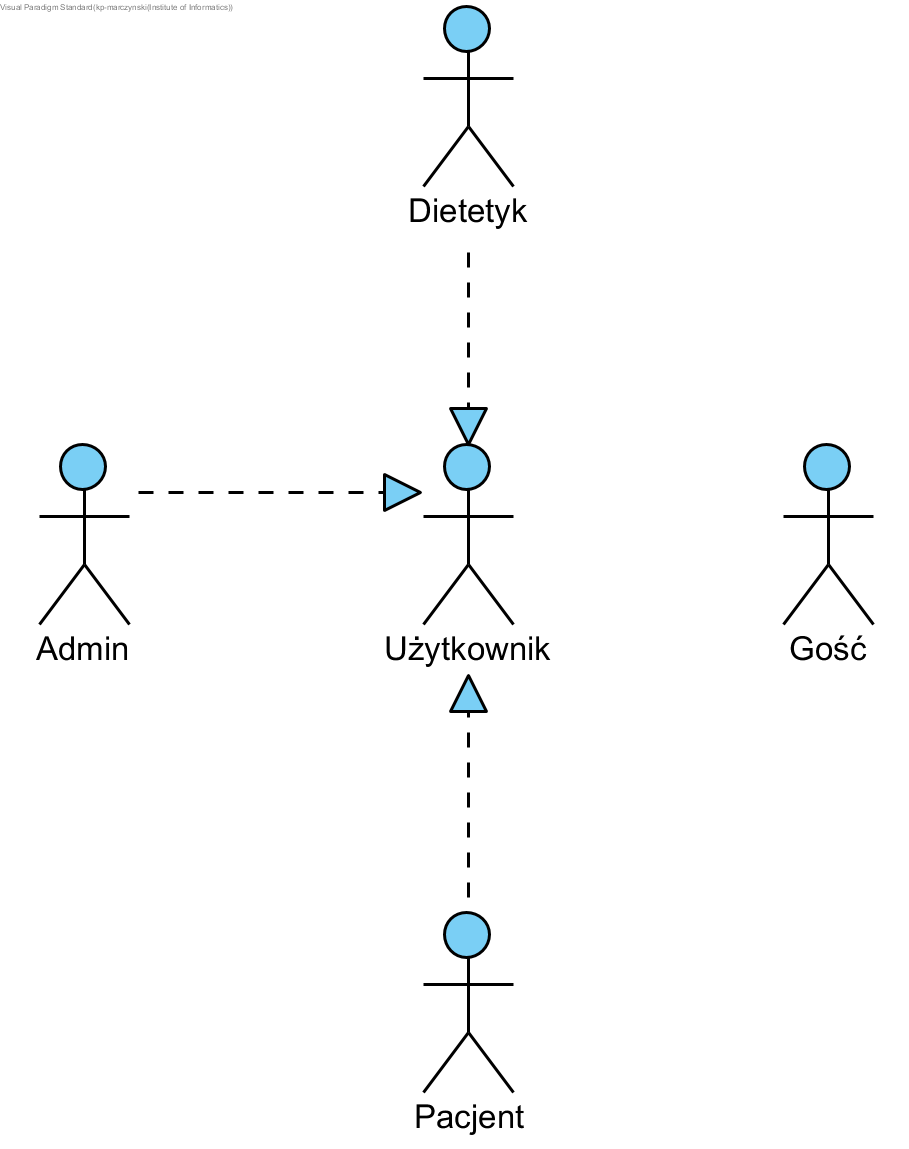
\includegraphics[scale=0.55]{../uml/use_case_diagrams/users.png}
        \caption{Użytkownicy - diagram przypadków użycia (opr.wł).}\label{rysunek:use-case-diagram-users}
    \end{figure}
\end{minipage}

\begin{minipage}{\textwidth}
    \begin{figure}[H]
        \centering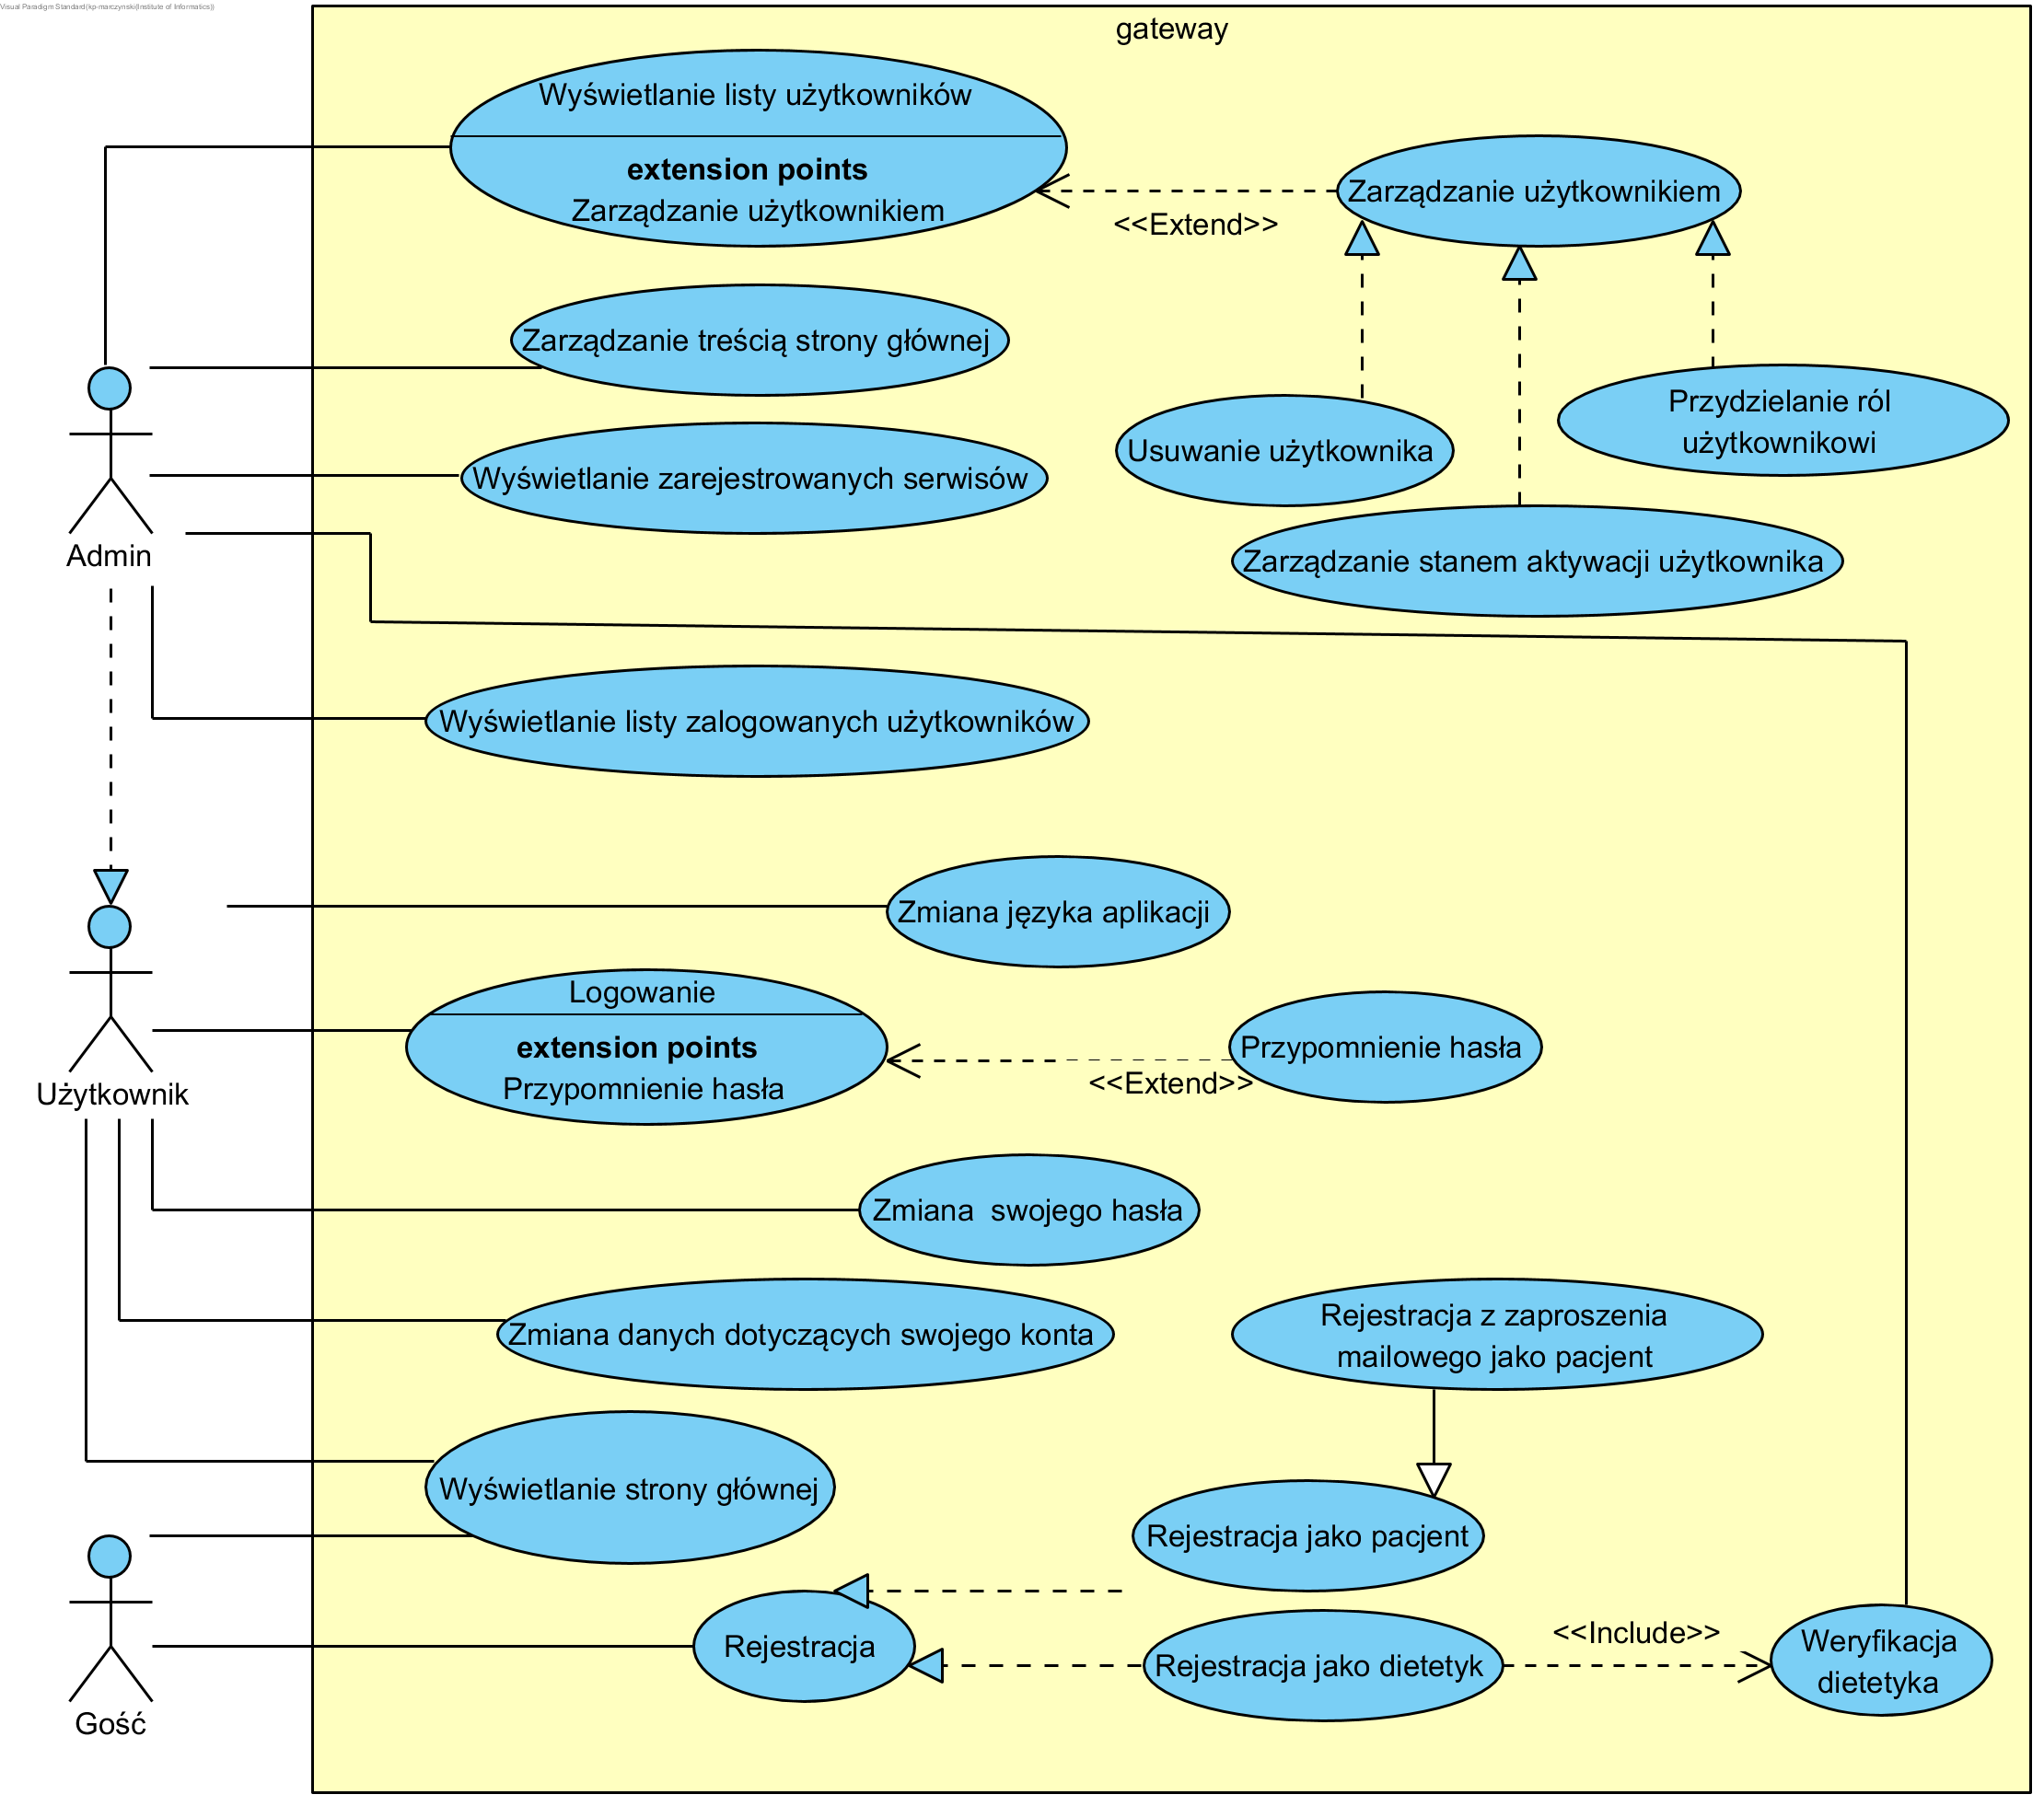
\includegraphics[scale=0.55]{../uml/use_case_diagrams/gateway.png}
        \caption{Gateway - diagram przypadków użycia (opr.wł).}\label{rysunek:use-case-diagram-gateway}
    \end{figure}
\end{minipage}

\begin{minipage}{\textwidth}
    \begin{figure}[H]
        \centering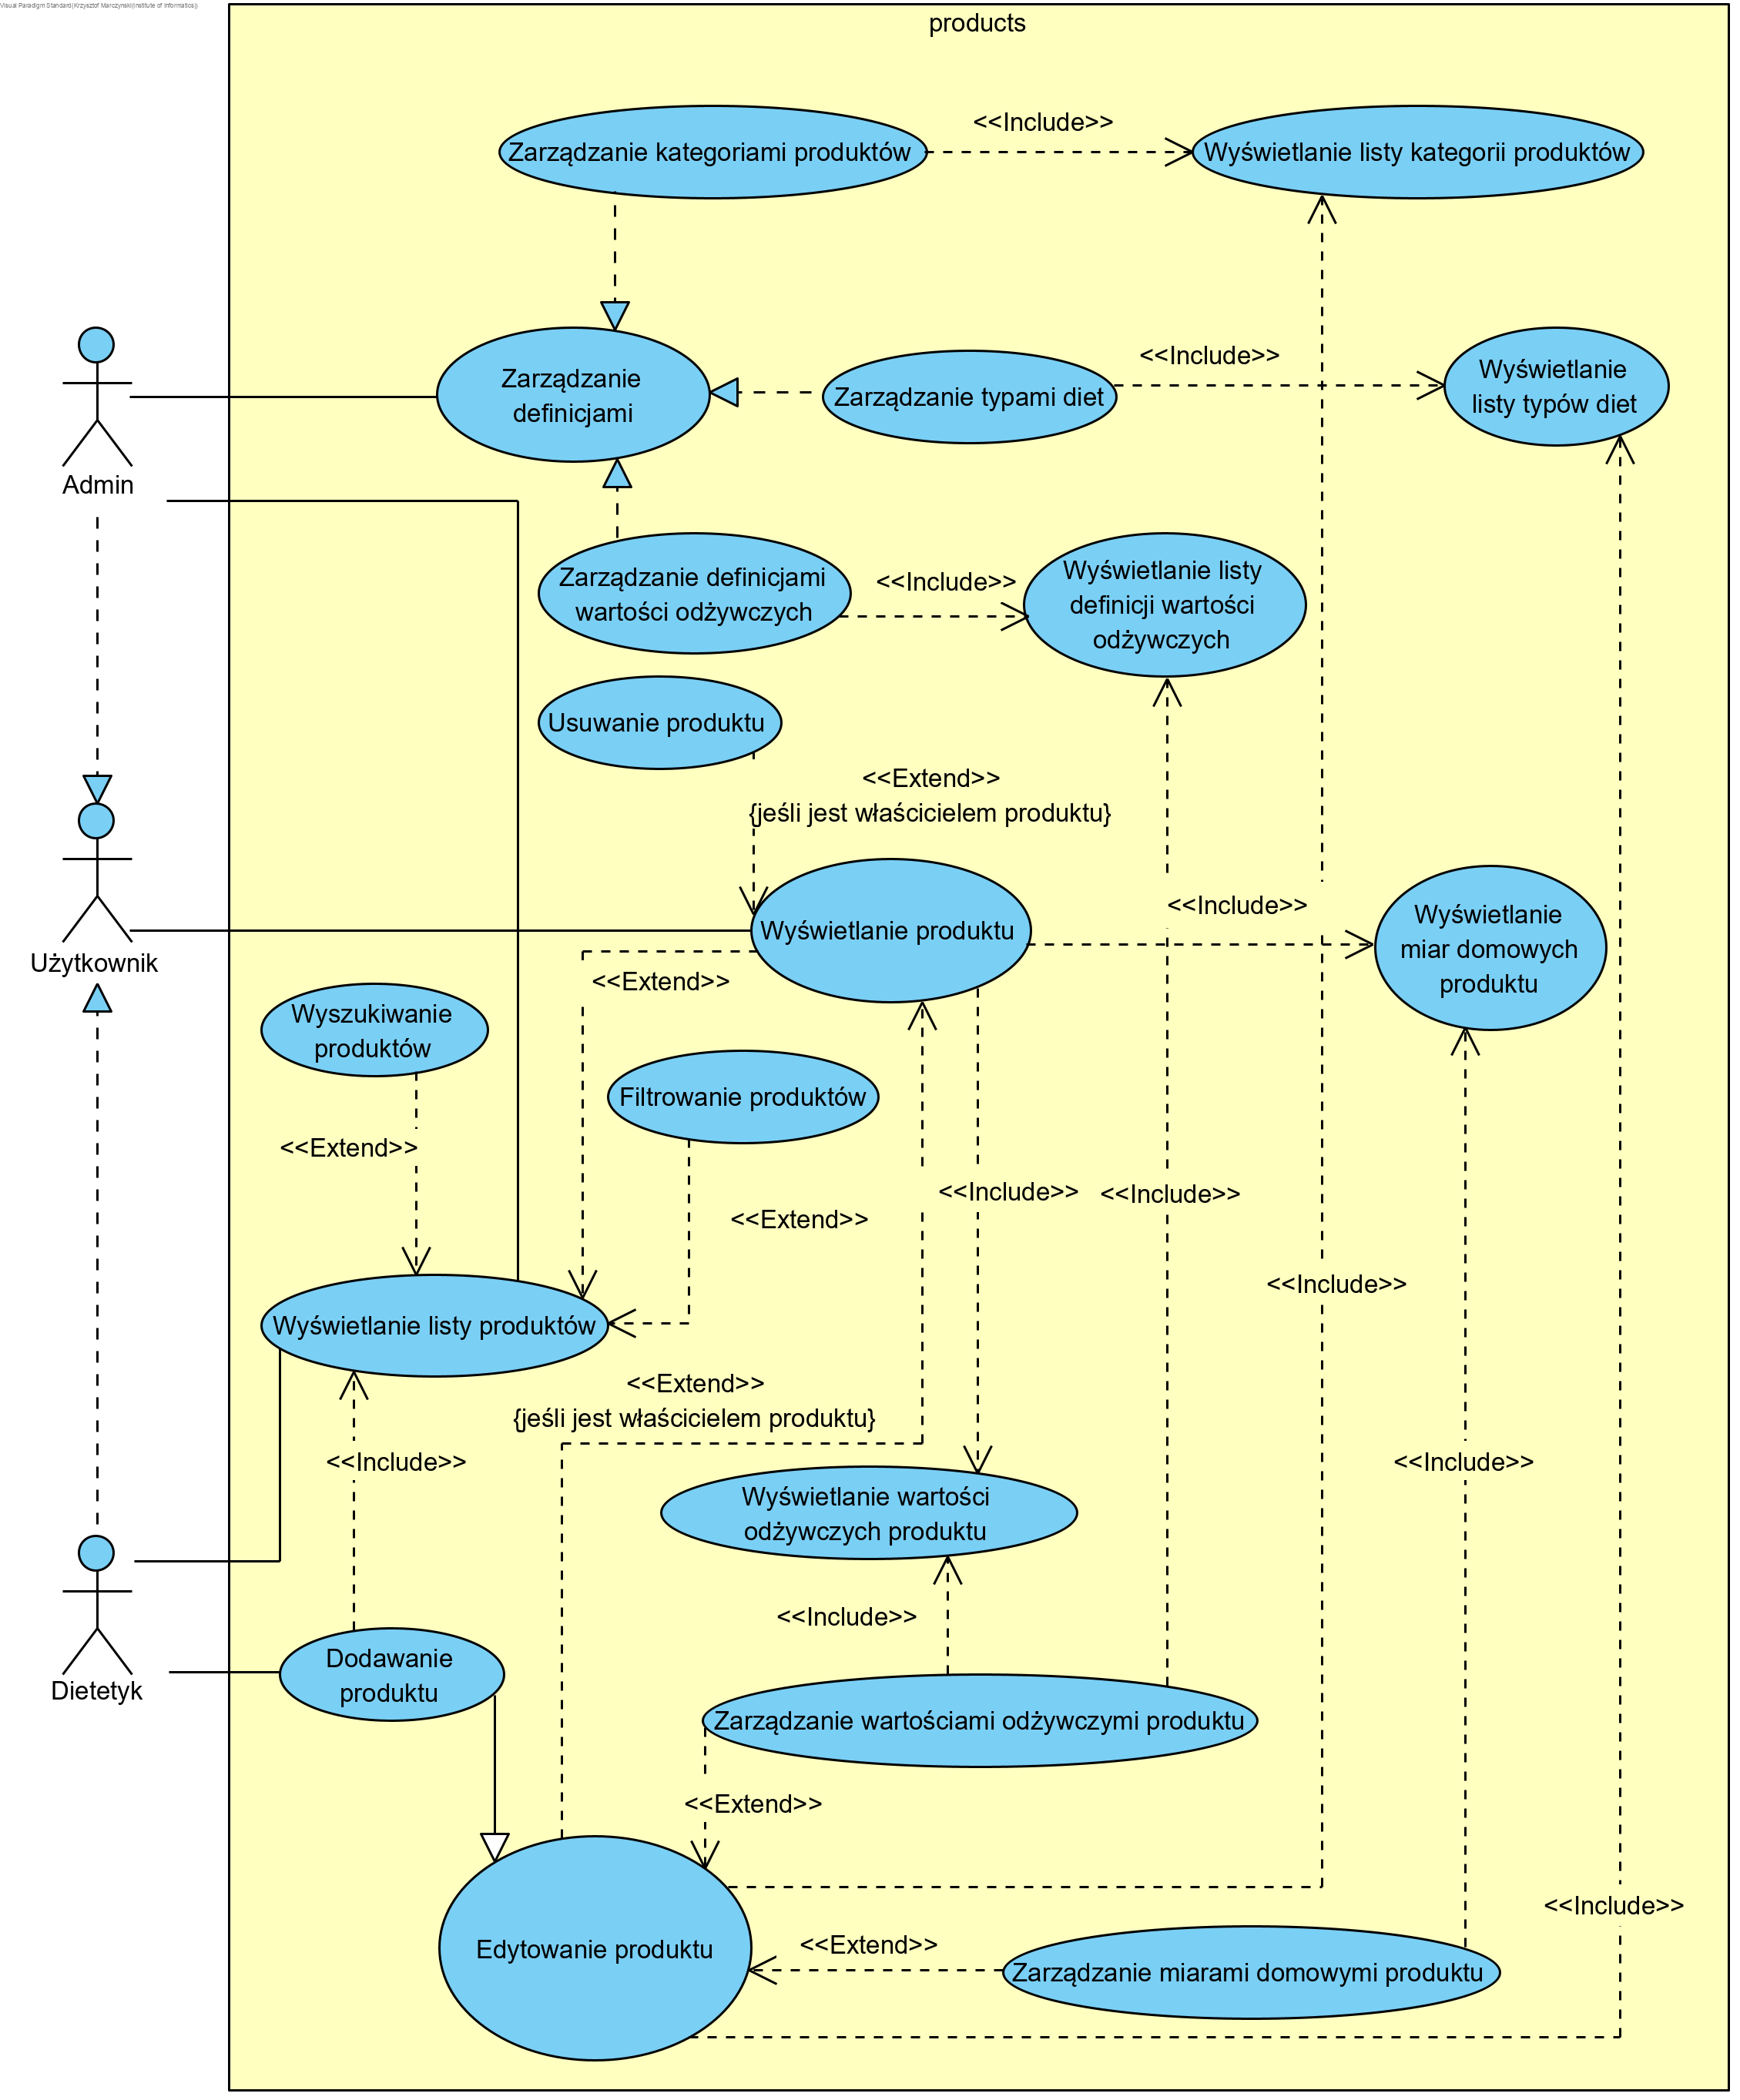
\includegraphics[scale=0.55]{../uml/use_case_diagrams/products.png}
        \caption{Produkty - diagram przypadków użycia (opr.wł).}\label{rysunek:use-case-diagram-products}
    \end{figure}
\end{minipage}

\begin{minipage}{\textwidth}
    \begin{figure}[H]
        \centering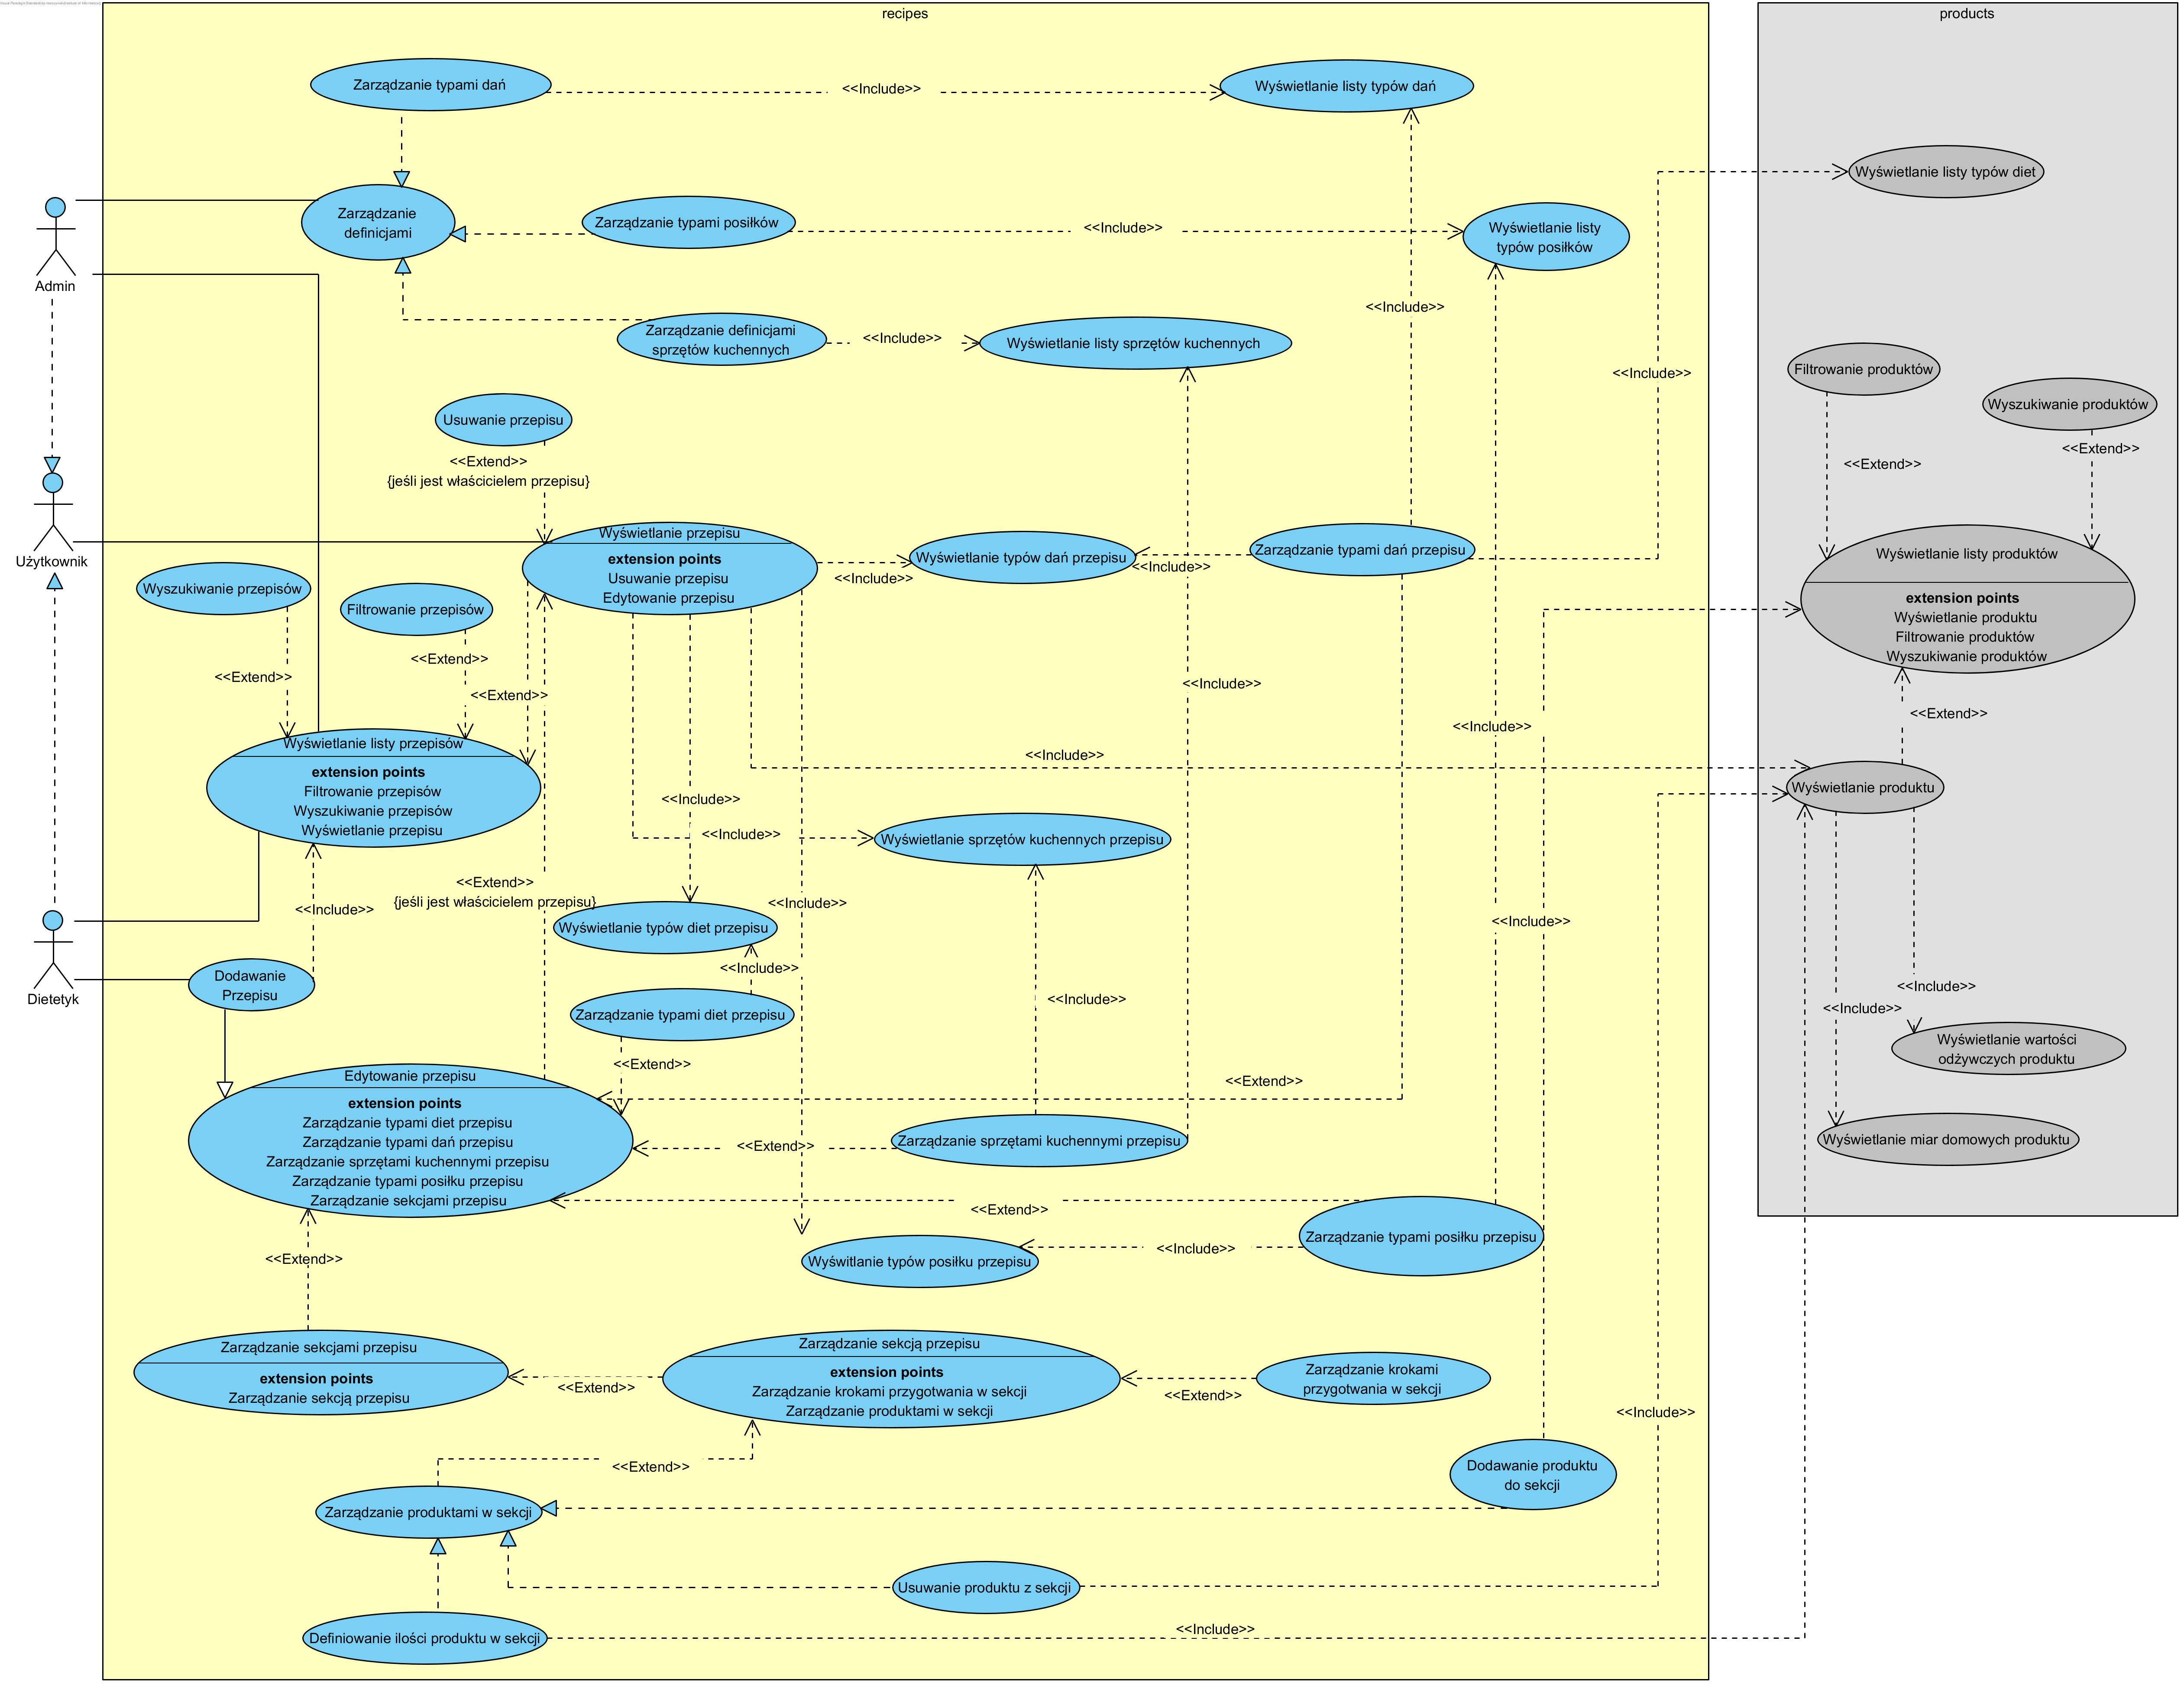
\includegraphics[scale=0.55]{../uml/use_case_diagrams/recipes.png}
        \caption{Przepisy - diagram przypadków użycia (opr.wł).}\label{rysunek:use-case-diagram-recipes}
    \end{figure}
\end{minipage}

\begin{minipage}{\textwidth}
    \begin{figure}[H]
        \centering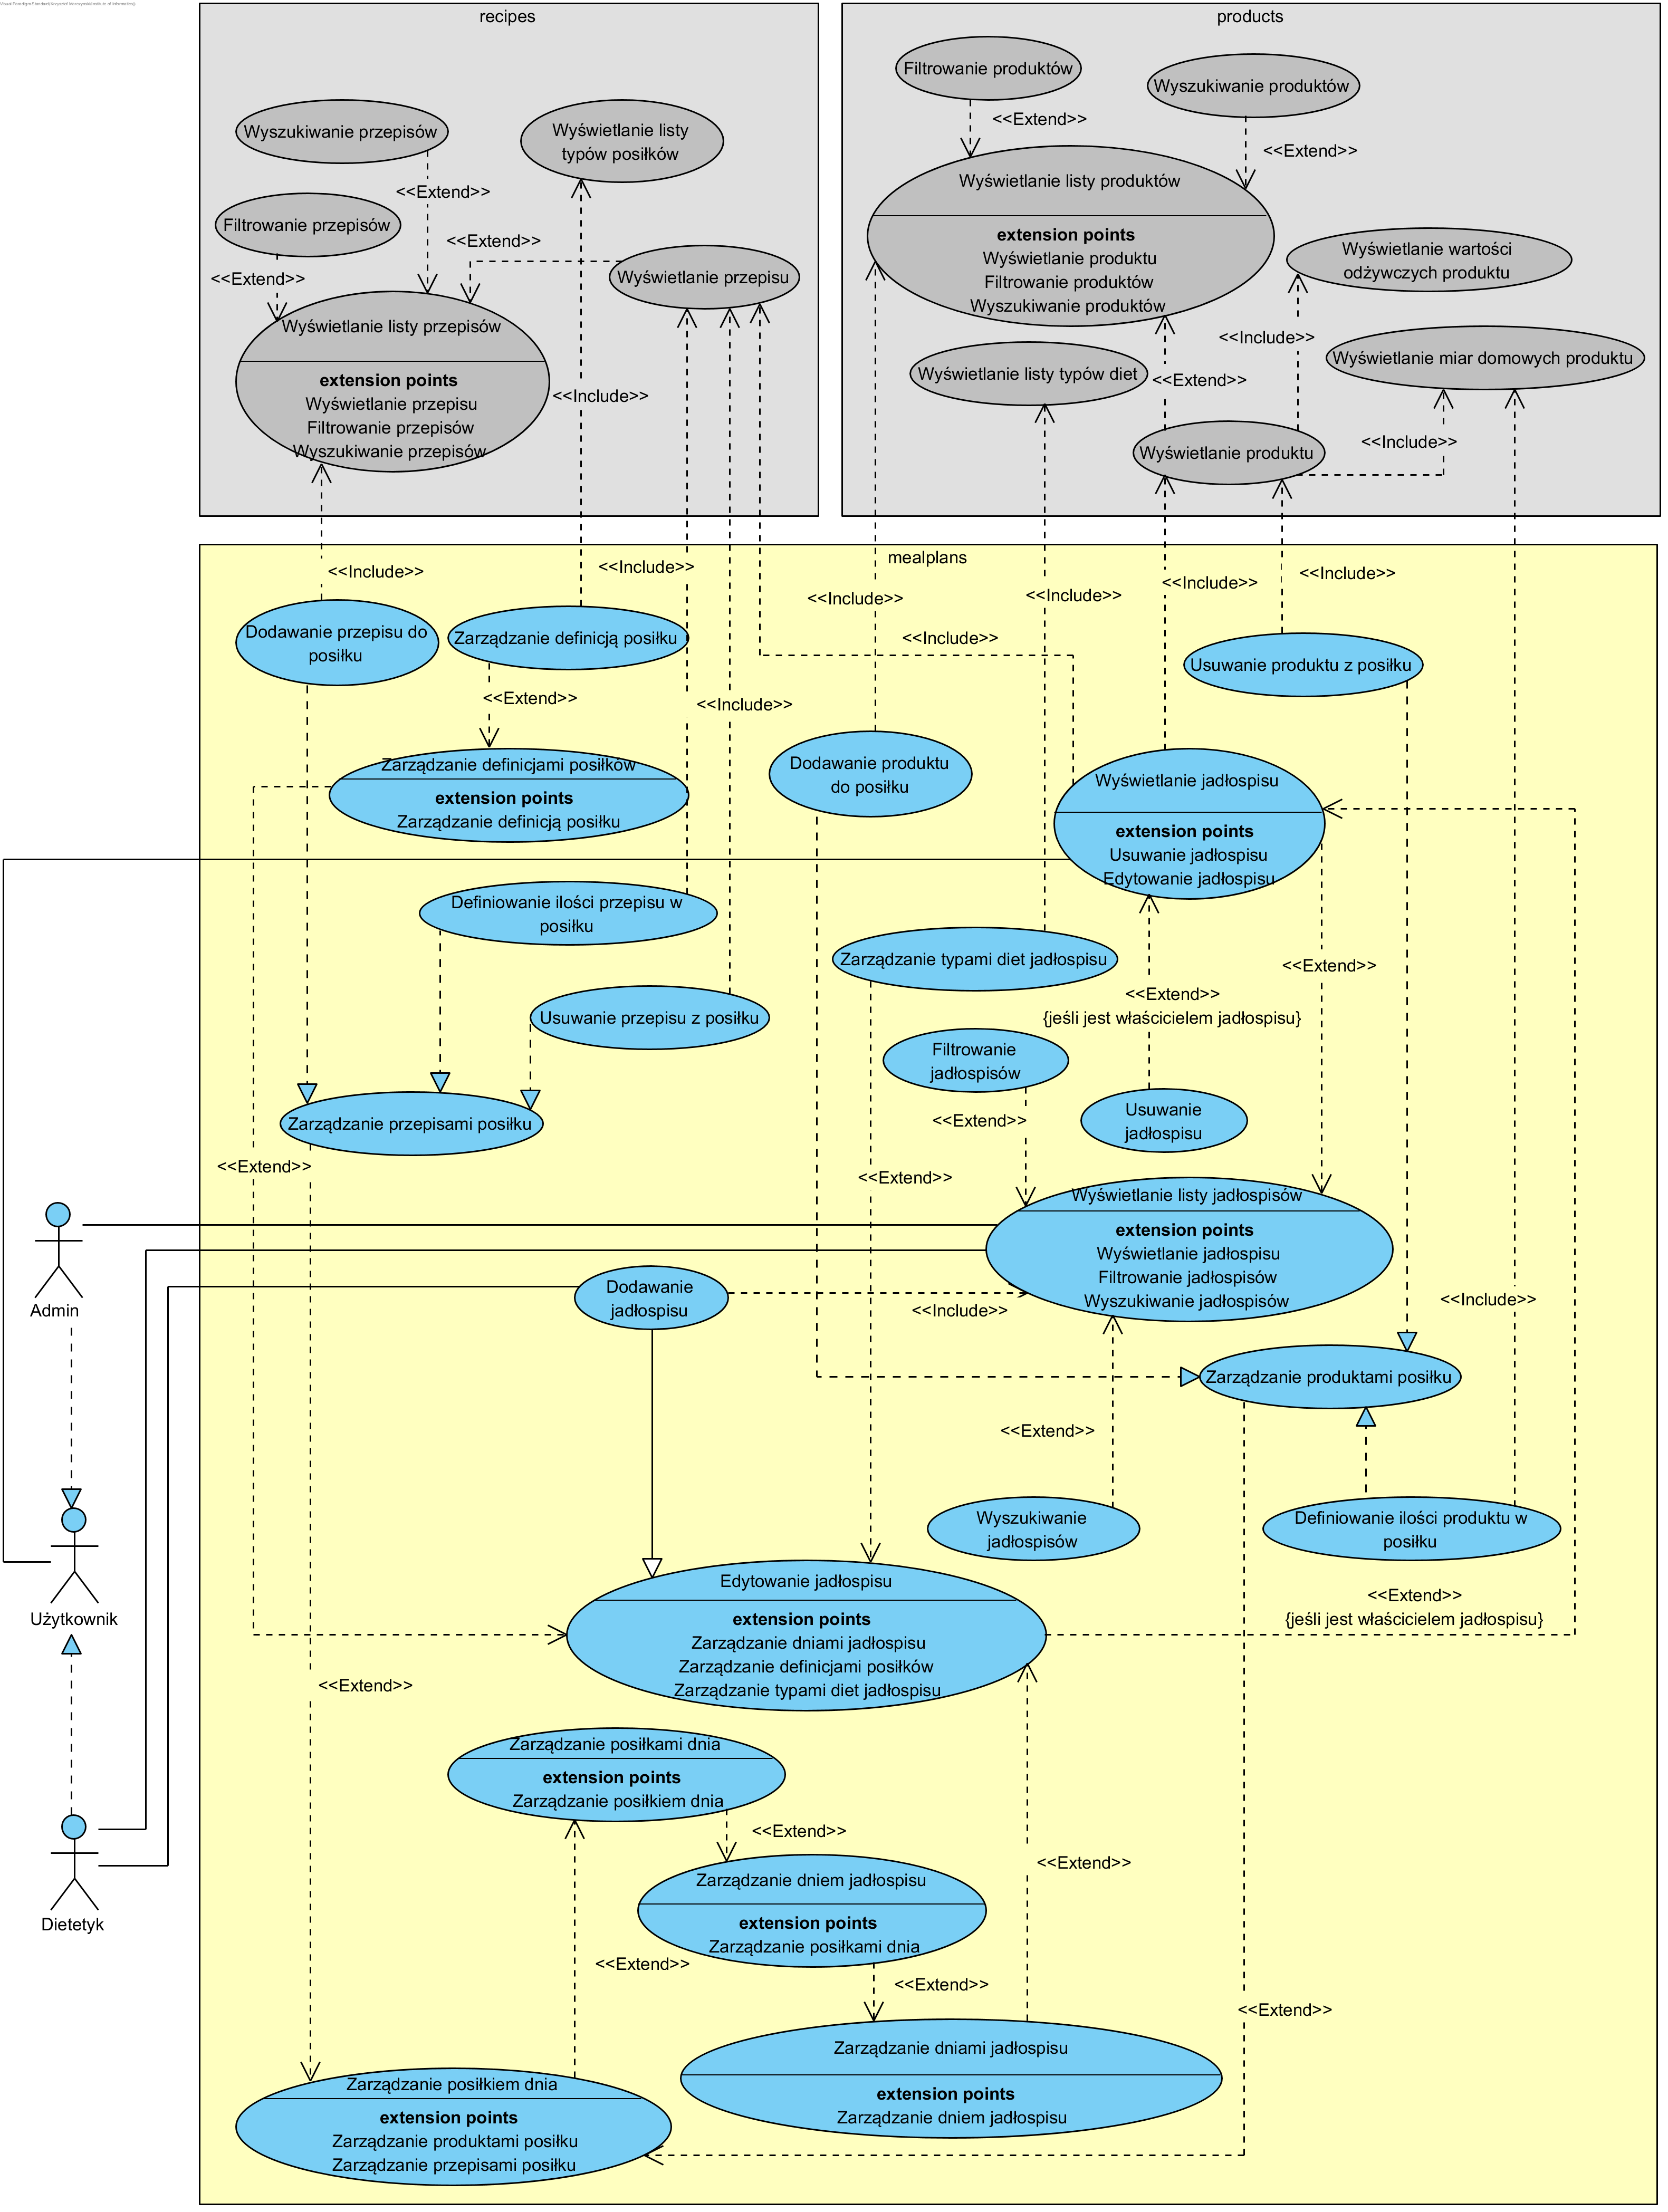
\includegraphics[scale=0.55]{../uml/use_case_diagrams/mealplans.png}
        \caption{Jadłospisy - diagram przypadków użycia (opr.wł).}\label{rysunek:use-case-diagram-mealplans}
    \end{figure}
\end{minipage}

\begin{minipage}{\textwidth}
    \begin{figure}[H]
        \centering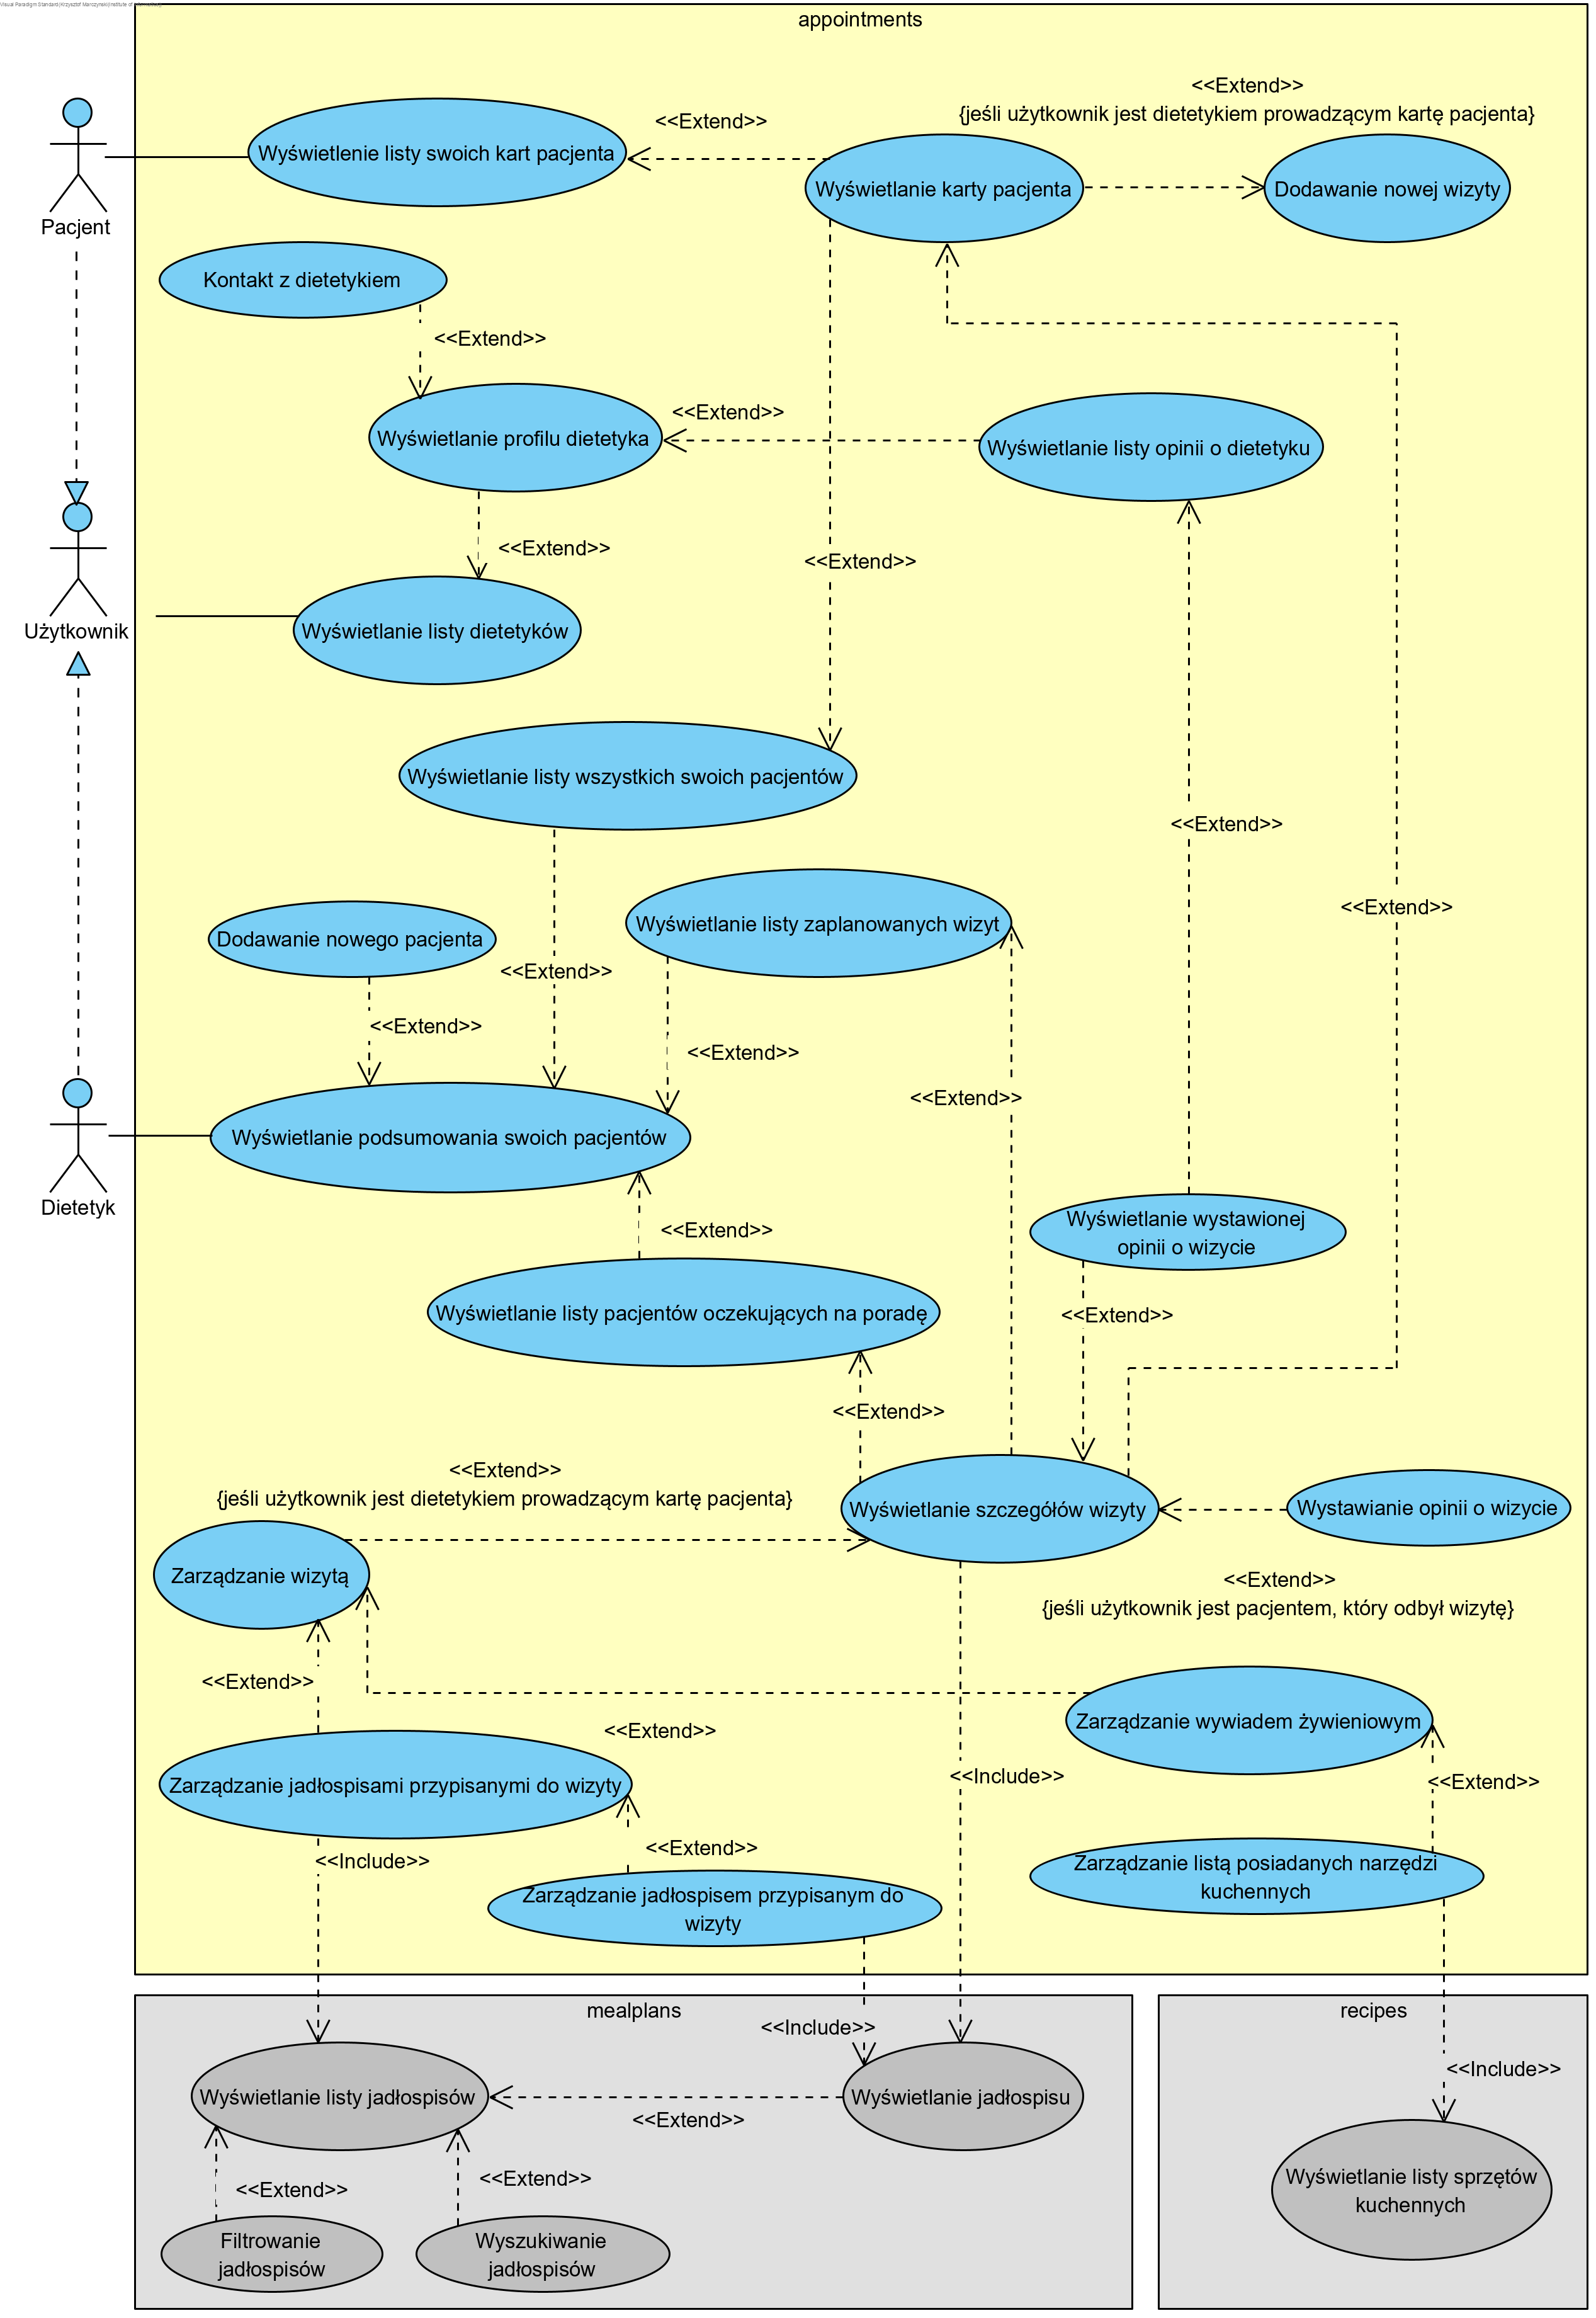
\includegraphics[scale=0.55]{../uml/use_case_diagrams/appointments.png}
        \caption{Wizyty - diagram przypadków użycia (opr.wł).}\label{rysunek:use-case-diagram-appointments}
    \end{figure}
\end{minipage}

\section{Prototyp interfejsu}
\todo{mockupy}
\begin{minipage}{\textwidth}
    \begin{figure}[H]
        \centering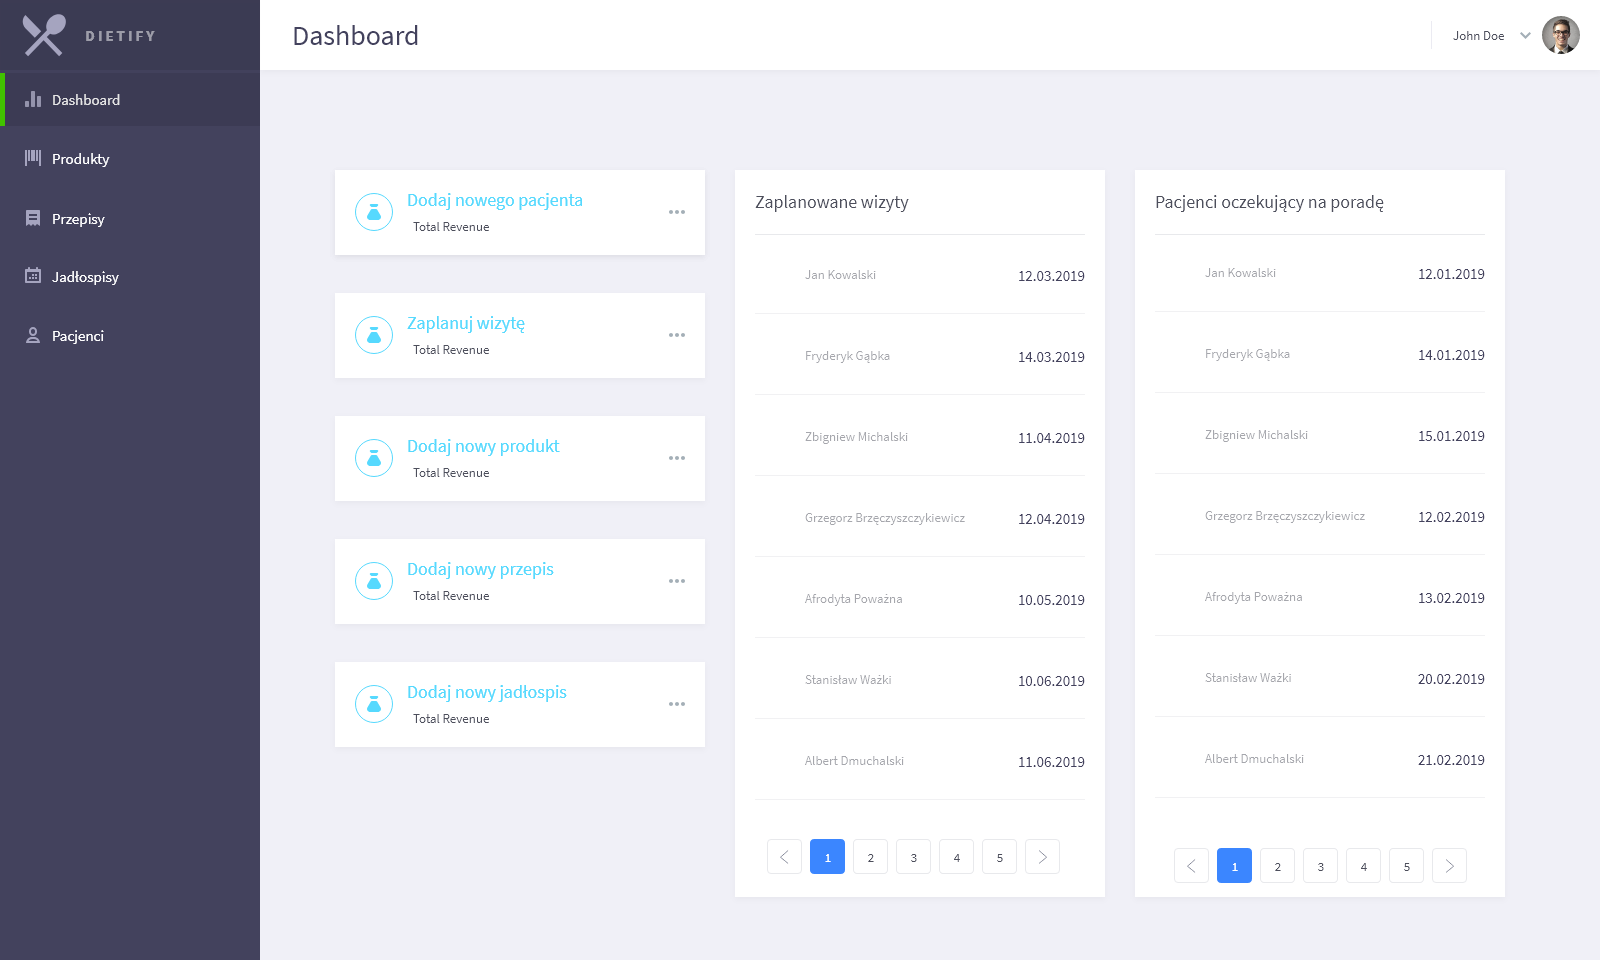
\includegraphics[width=0.9\textwidth]{img/mockups/mockup1.png}
        \caption{Mockup1 (opr.wł).}\label{rysunek:mockup1}
    \end{figure}
\end{minipage}

\begin{minipage}{\textwidth}
    \begin{figure}[H]
        \centering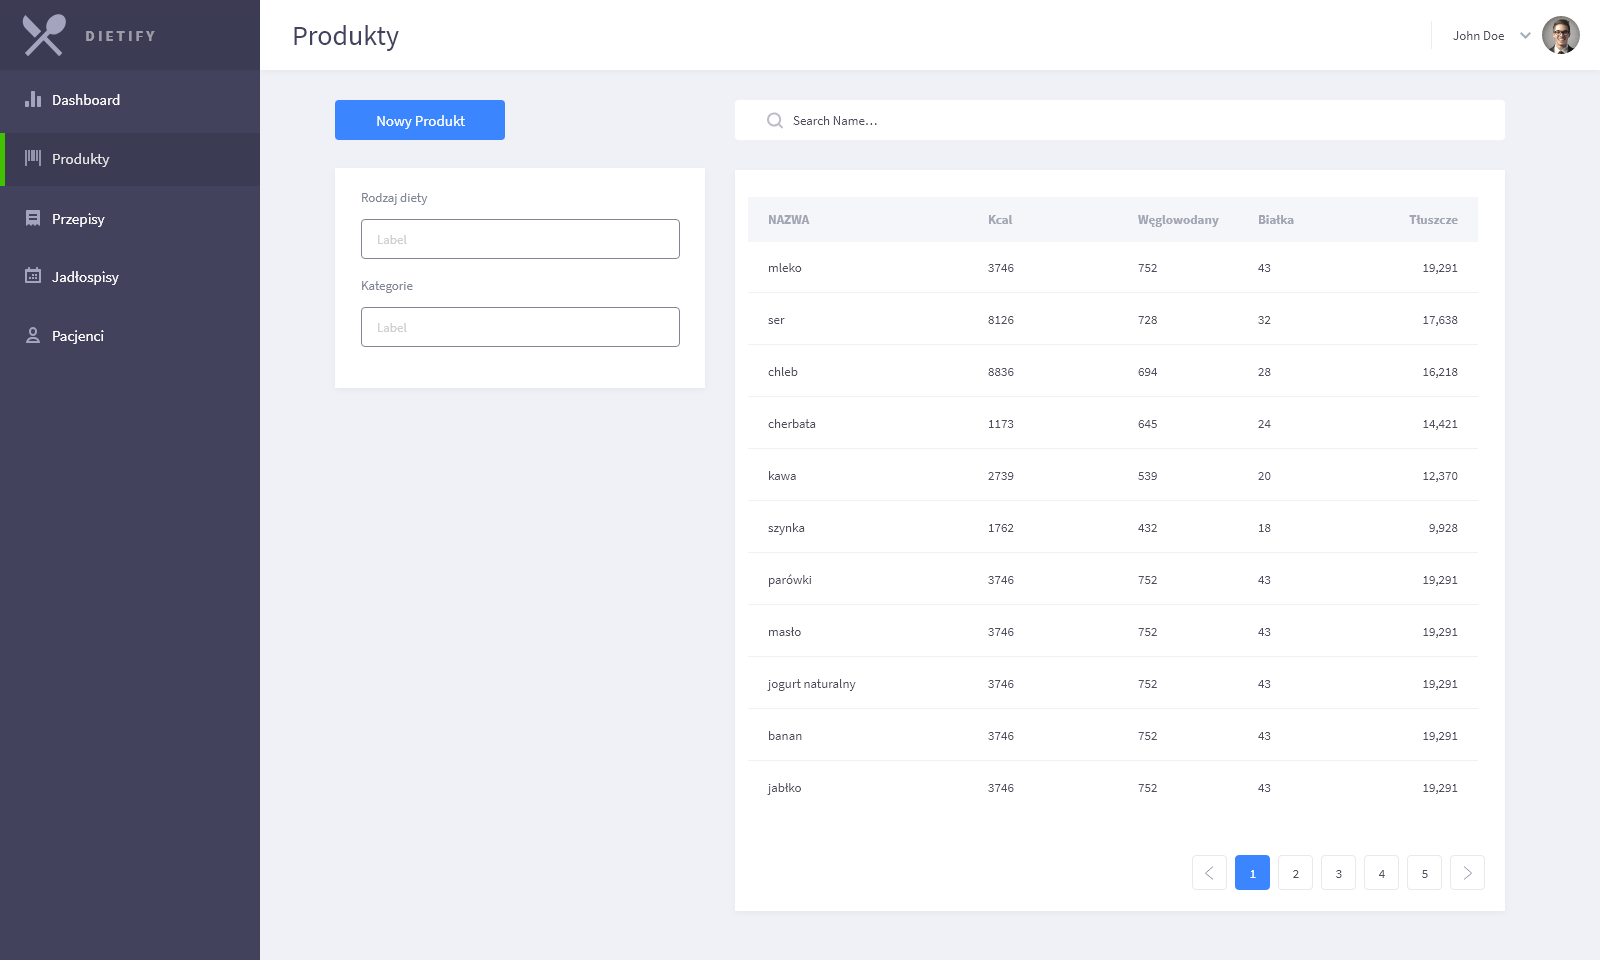
\includegraphics[width=0.9\textwidth]{img/mockups/mockup2.png}
        \caption{Mockup2 (opr.wł).}\label{rysunek:mockup2}
    \end{figure}
\end{minipage}

\begin{minipage}{\textwidth}
    \begin{figure}[H]
        \centering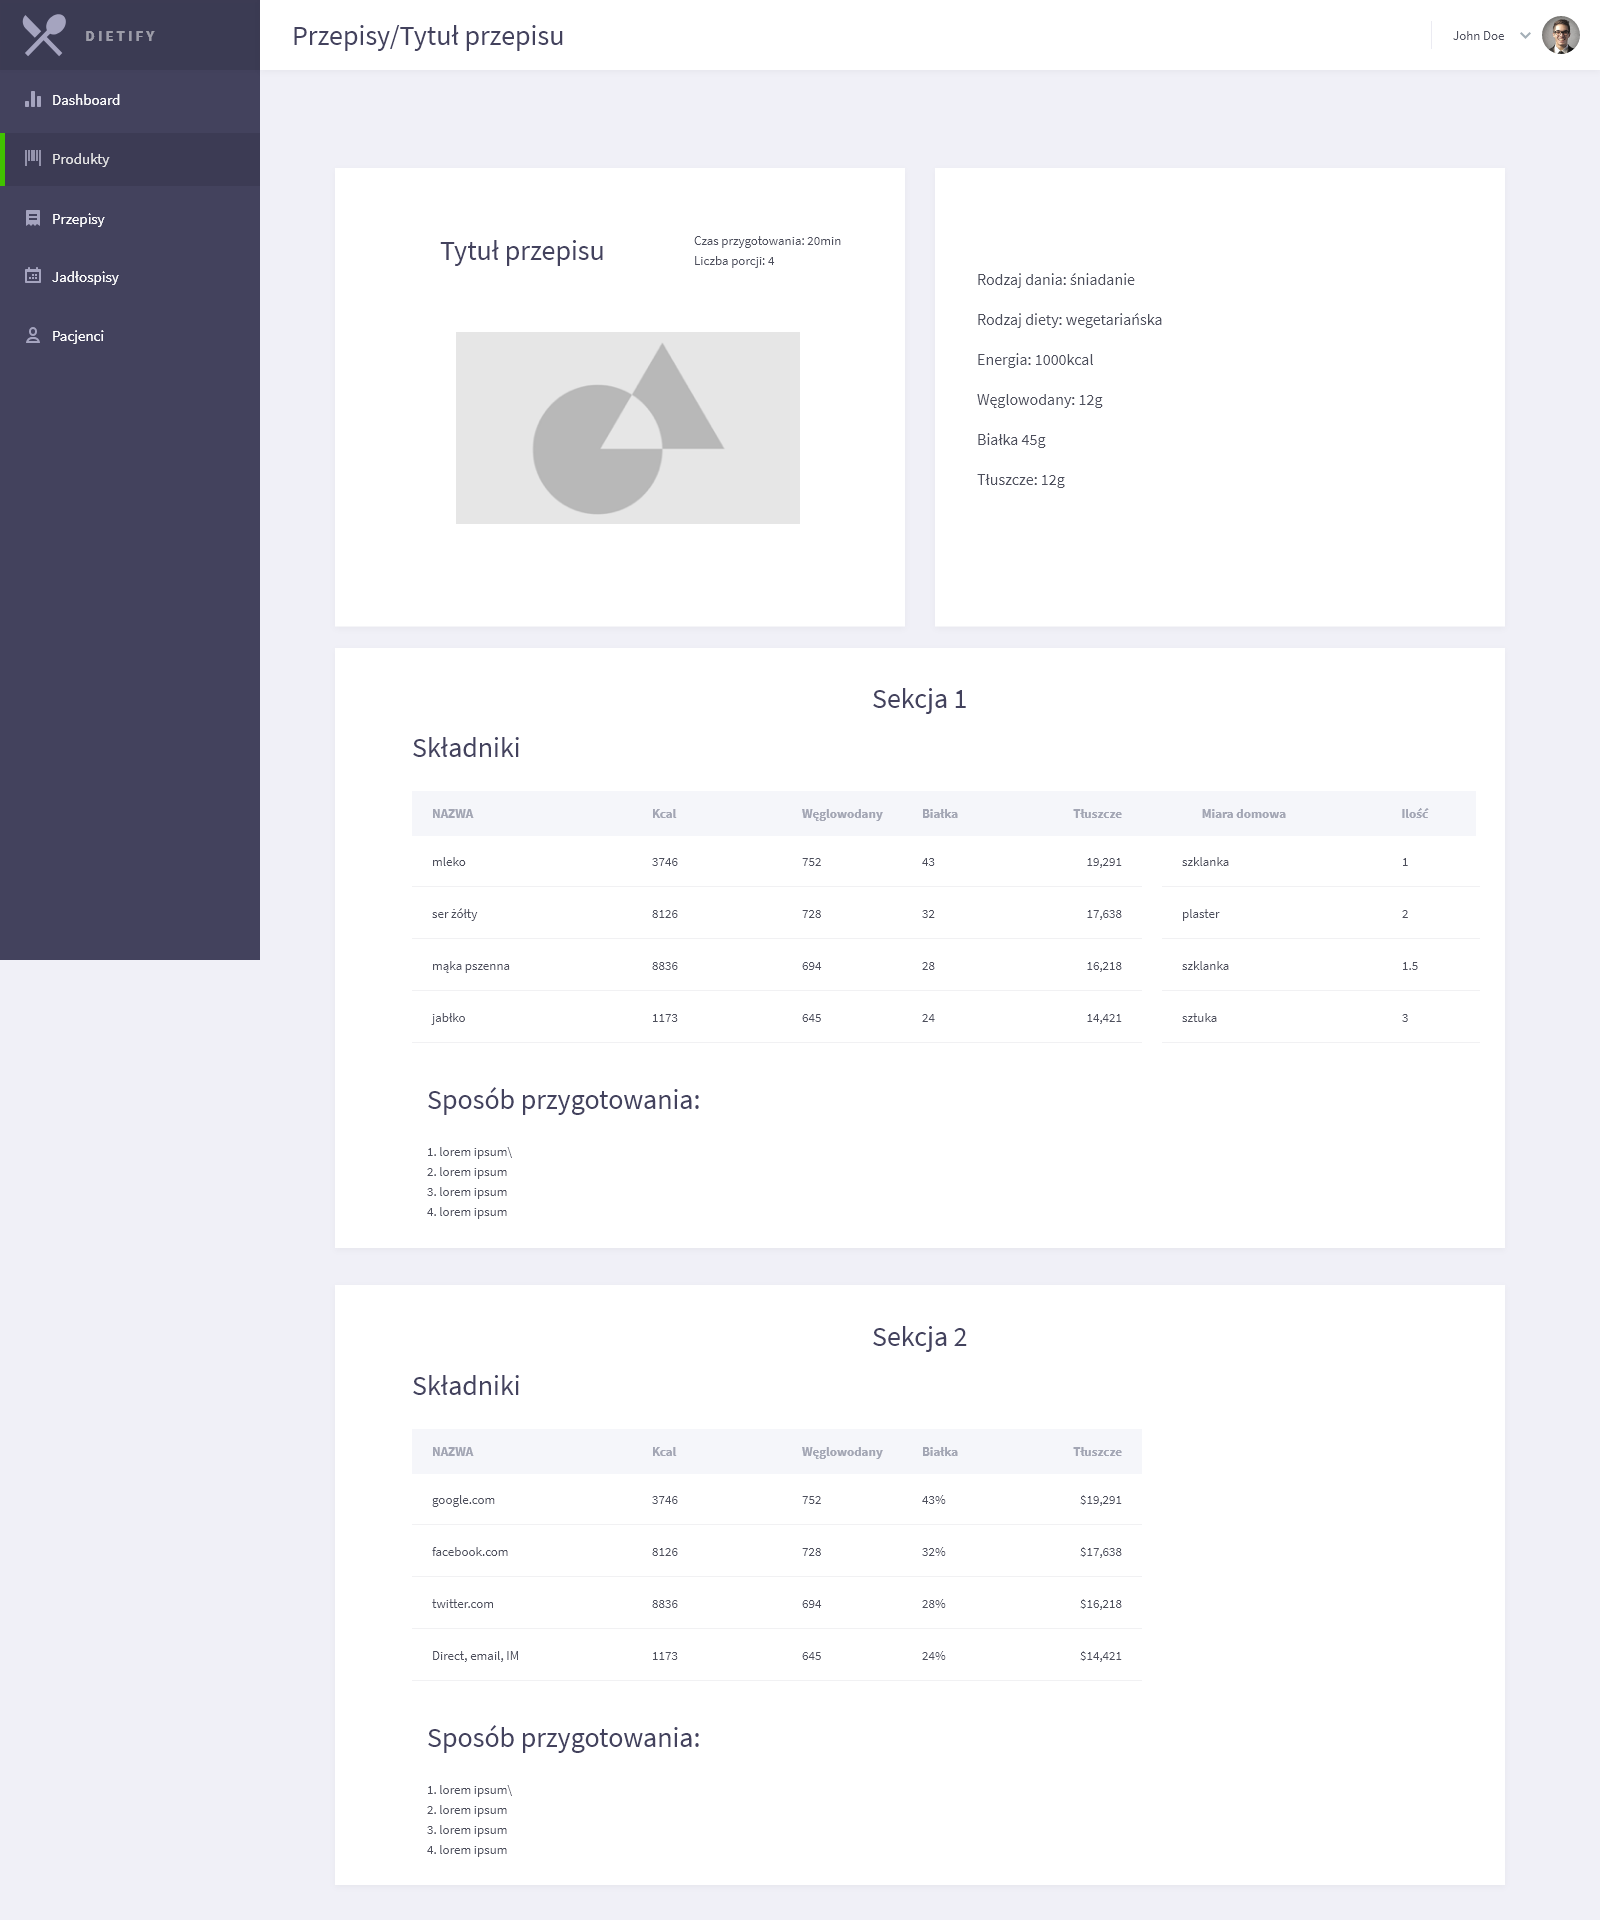
\includegraphics[width=0.9\textwidth]{img/mockups/mockup3.png}
        \caption{Mockup3 (opr.wł).}\label{rysunek:mockup3}
    \end{figure}
\end{minipage}

\begin{minipage}{\textwidth}
    \begin{figure}[H]
        \centering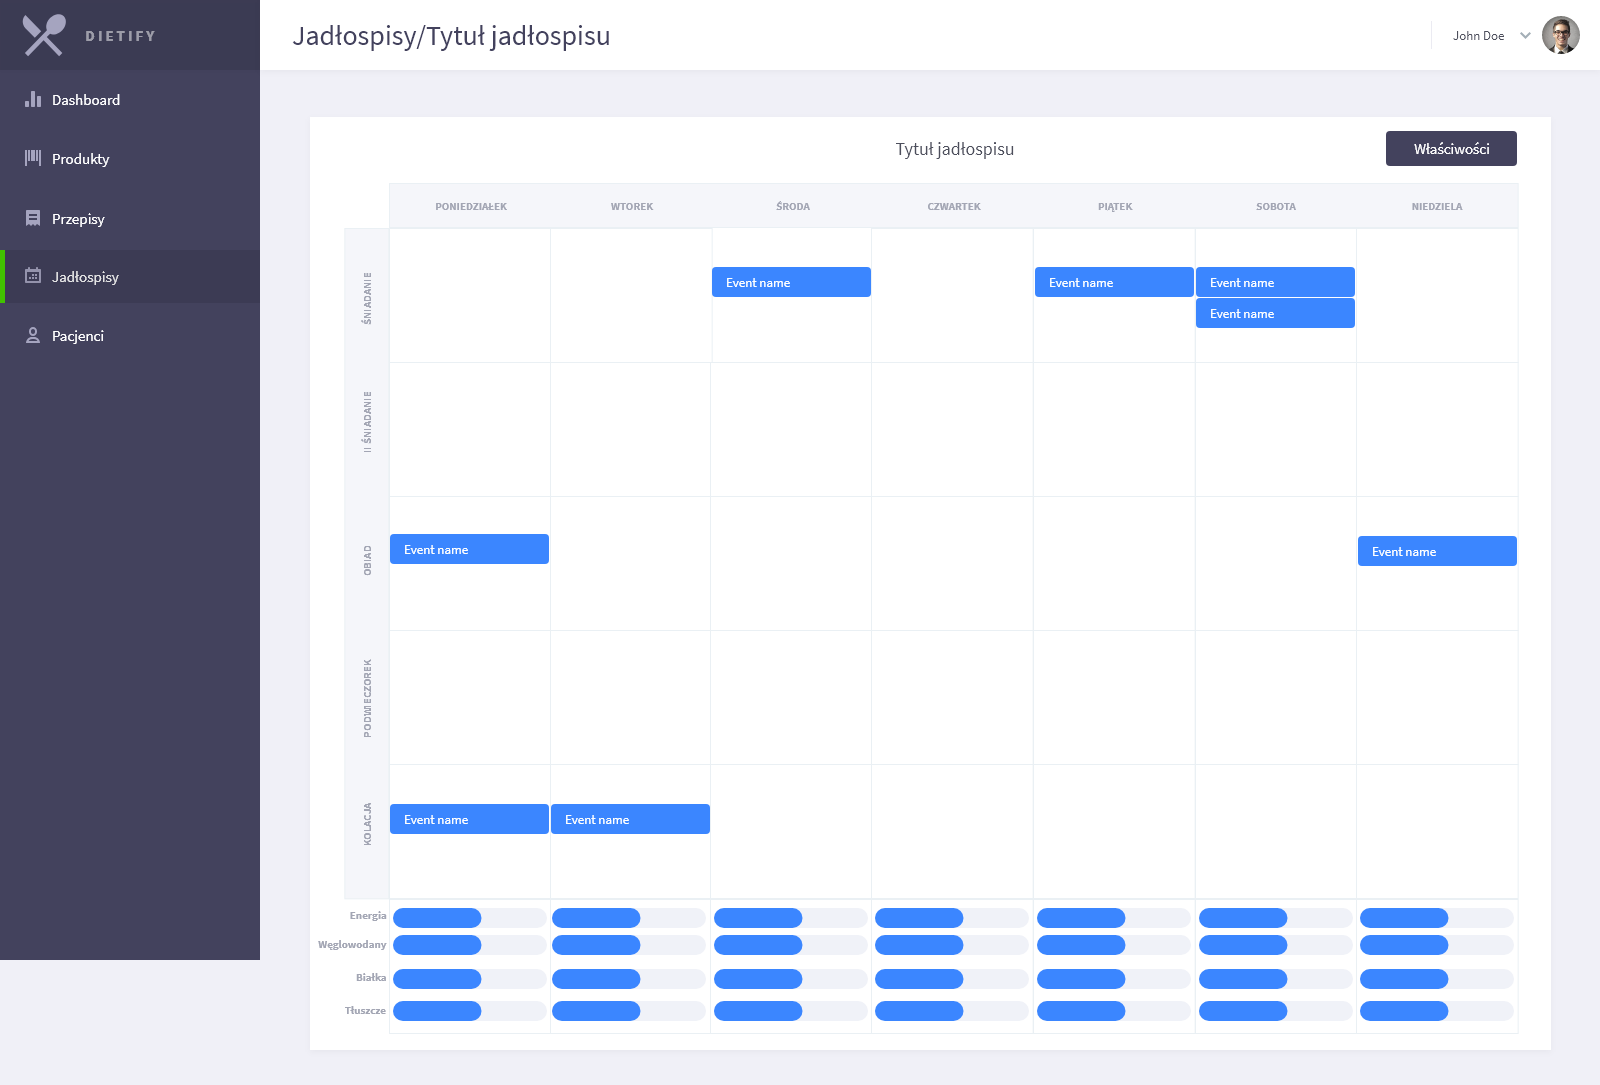
\includegraphics[width=0.9\textwidth]{img/mockups/mockup4.png}
        \caption{Mockup4 (opr.wł).}\label{rysunek:mockup4}
    \end{figure}
\end{minipage}

\begin{minipage}{\textwidth}
    \begin{figure}[H]
        \centering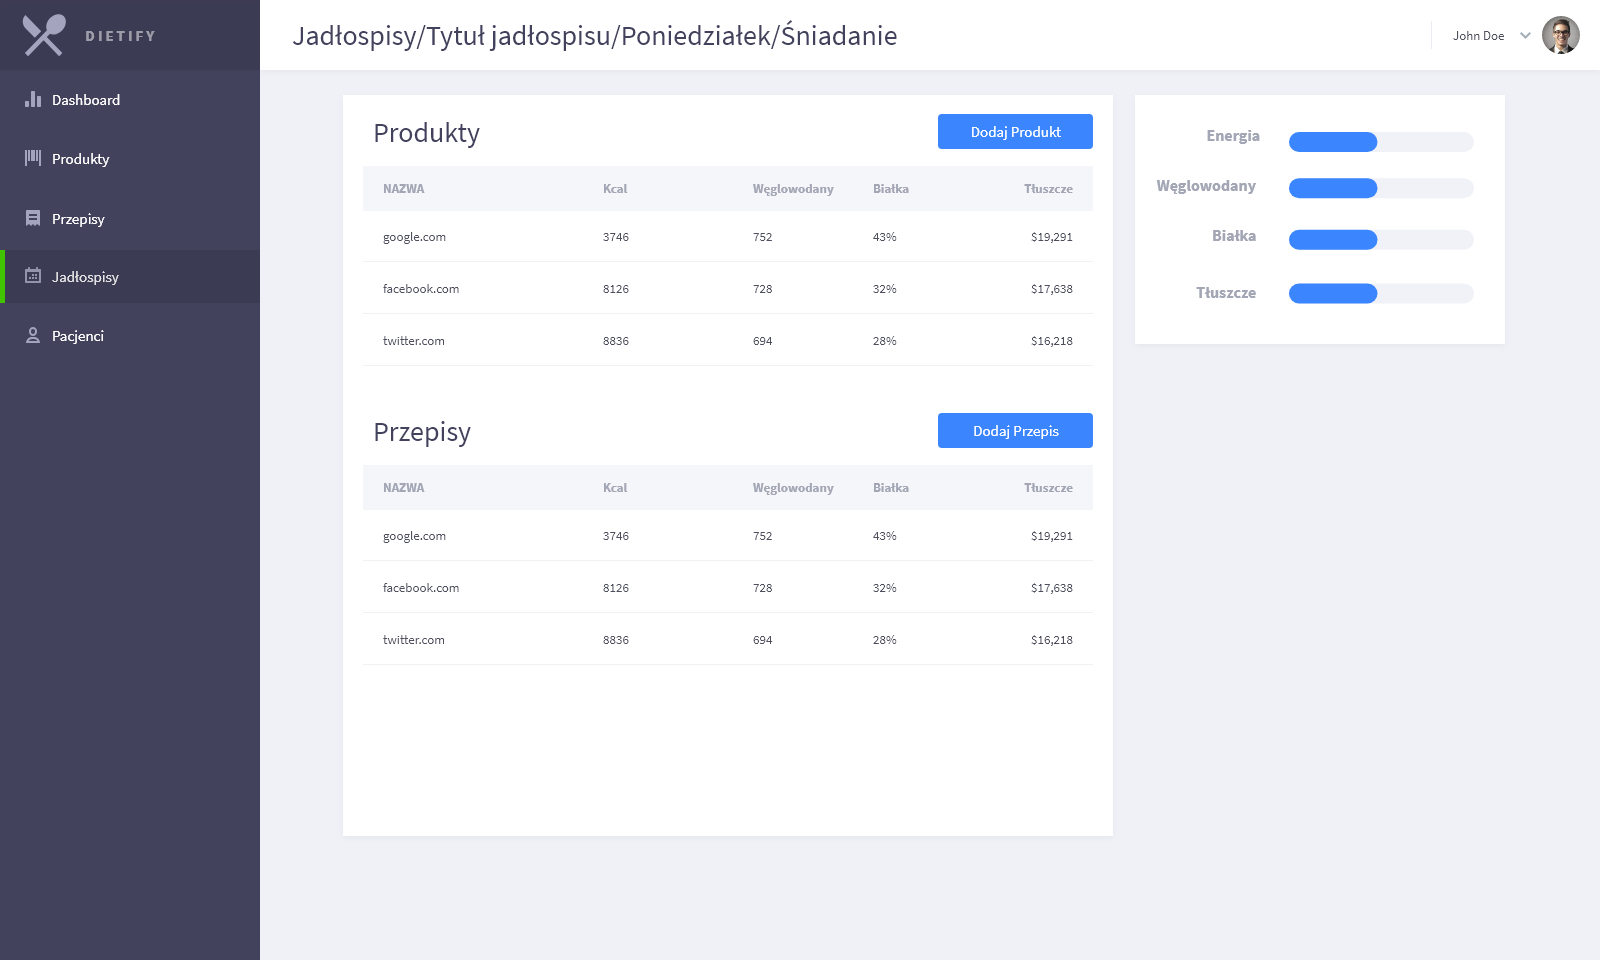
\includegraphics[width=0.9\textwidth]{img/mockups/mockup5.png}
        \caption{Mockup5 (opr.wł).}\label{rysunek:mockup5}
    \end{figure}
\end{minipage}

\begin{minipage}{\textwidth}
    \begin{figure}[H]
        \centering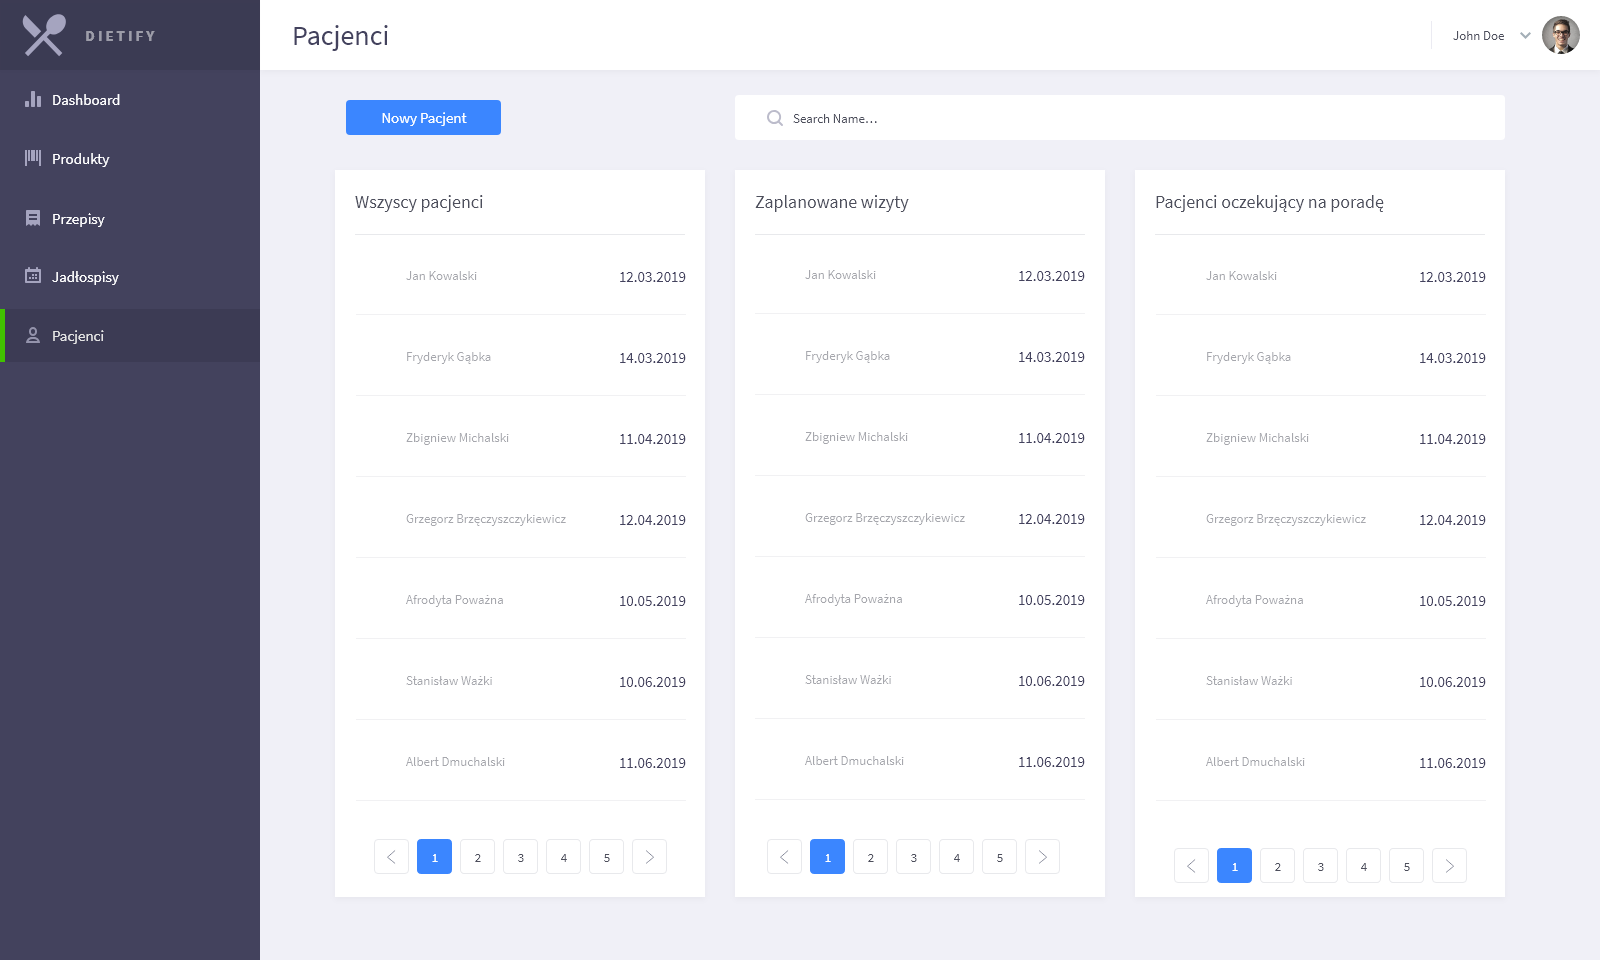
\includegraphics[width=0.9\textwidth]{img/mockups/mockup6.png}
        \caption{Mockup6 (opr.wł).}\label{rysunek:mockup6}
    \end{figure}
\end{minipage}

\begin{minipage}{\textwidth}
    \begin{figure}[H]
        \centering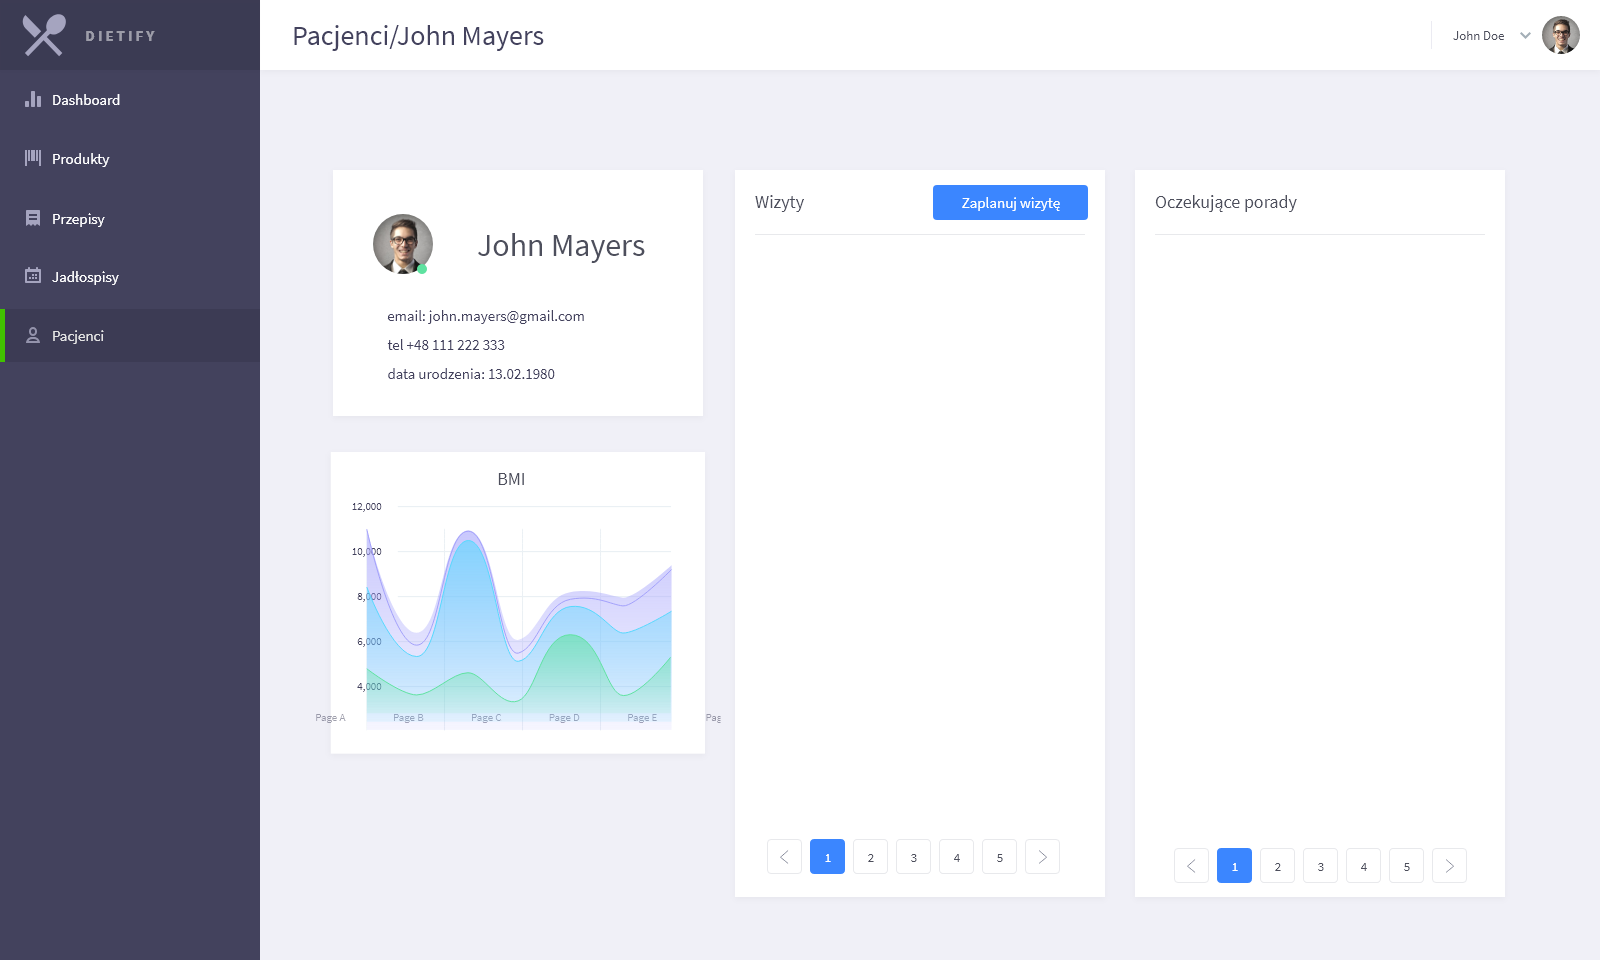
\includegraphics[width=0.9\textwidth]{img/mockups/mockup7.png}
        \caption{Mockup7 (opr.wł).}\label{rysunek:mockup7}
    \end{figure}
\end{minipage}

\begin{minipage}{\textwidth}
    \begin{figure}[H]
        \centering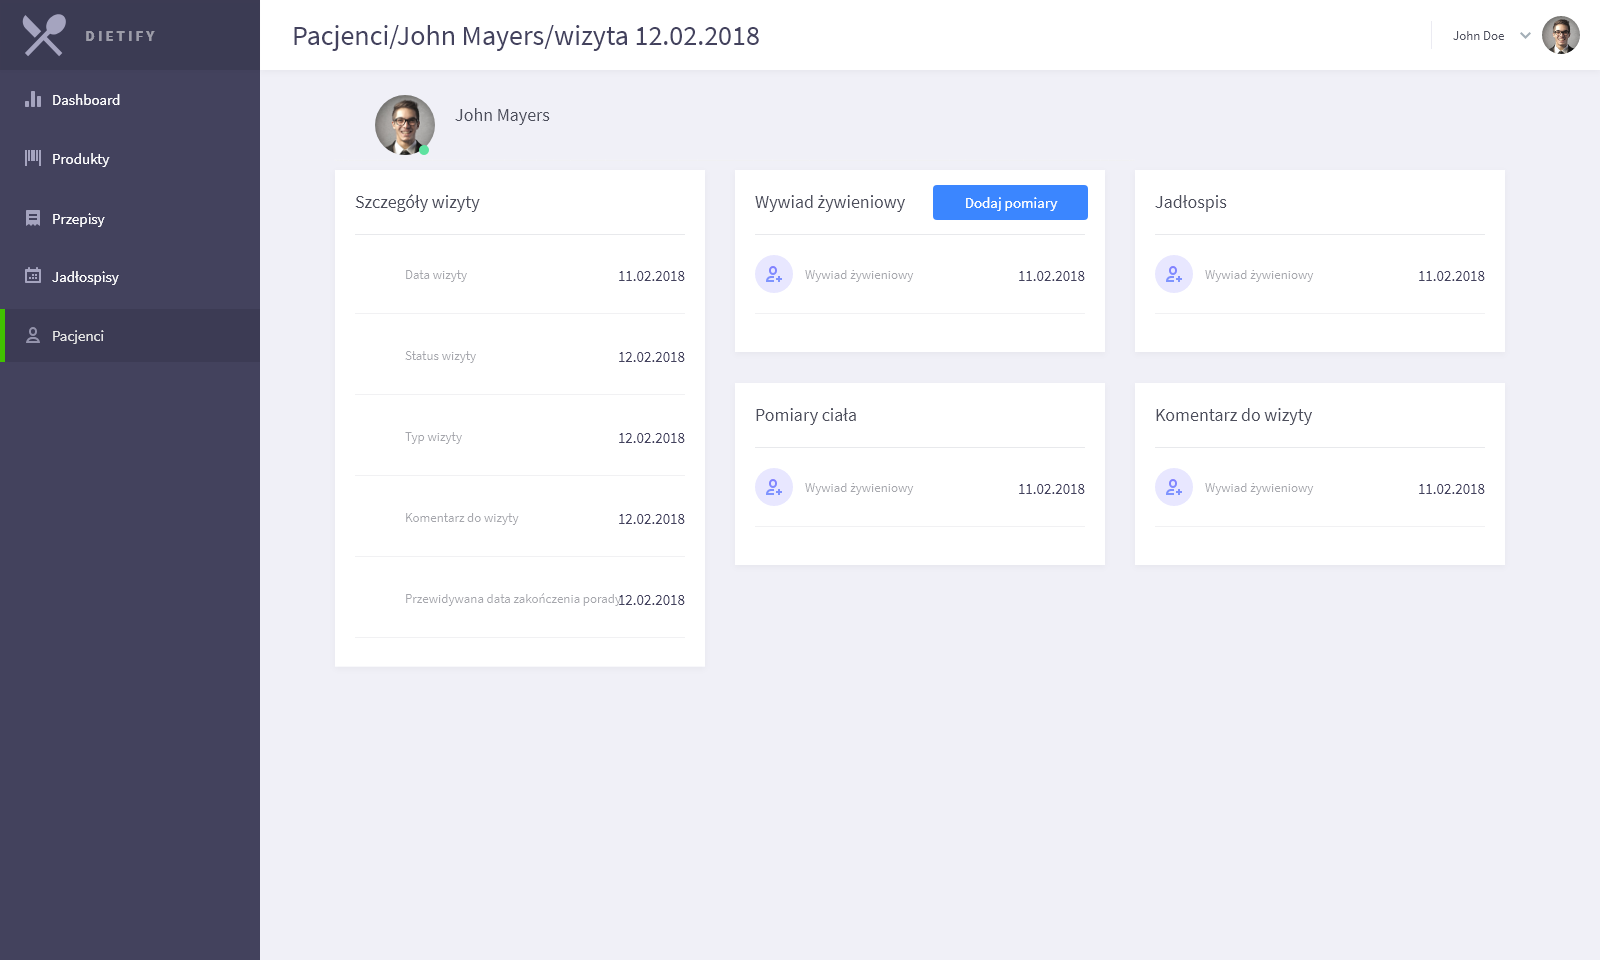
\includegraphics[width=0.9\textwidth]{img/mockups/mockup8.png}
        \caption{Mockup8 (opr.wł).}\label{rysunek:mockup8}
    \end{figure}
\end{minipage}

\begin{minipage}{\textwidth}
    \begin{figure}[H]
        \centering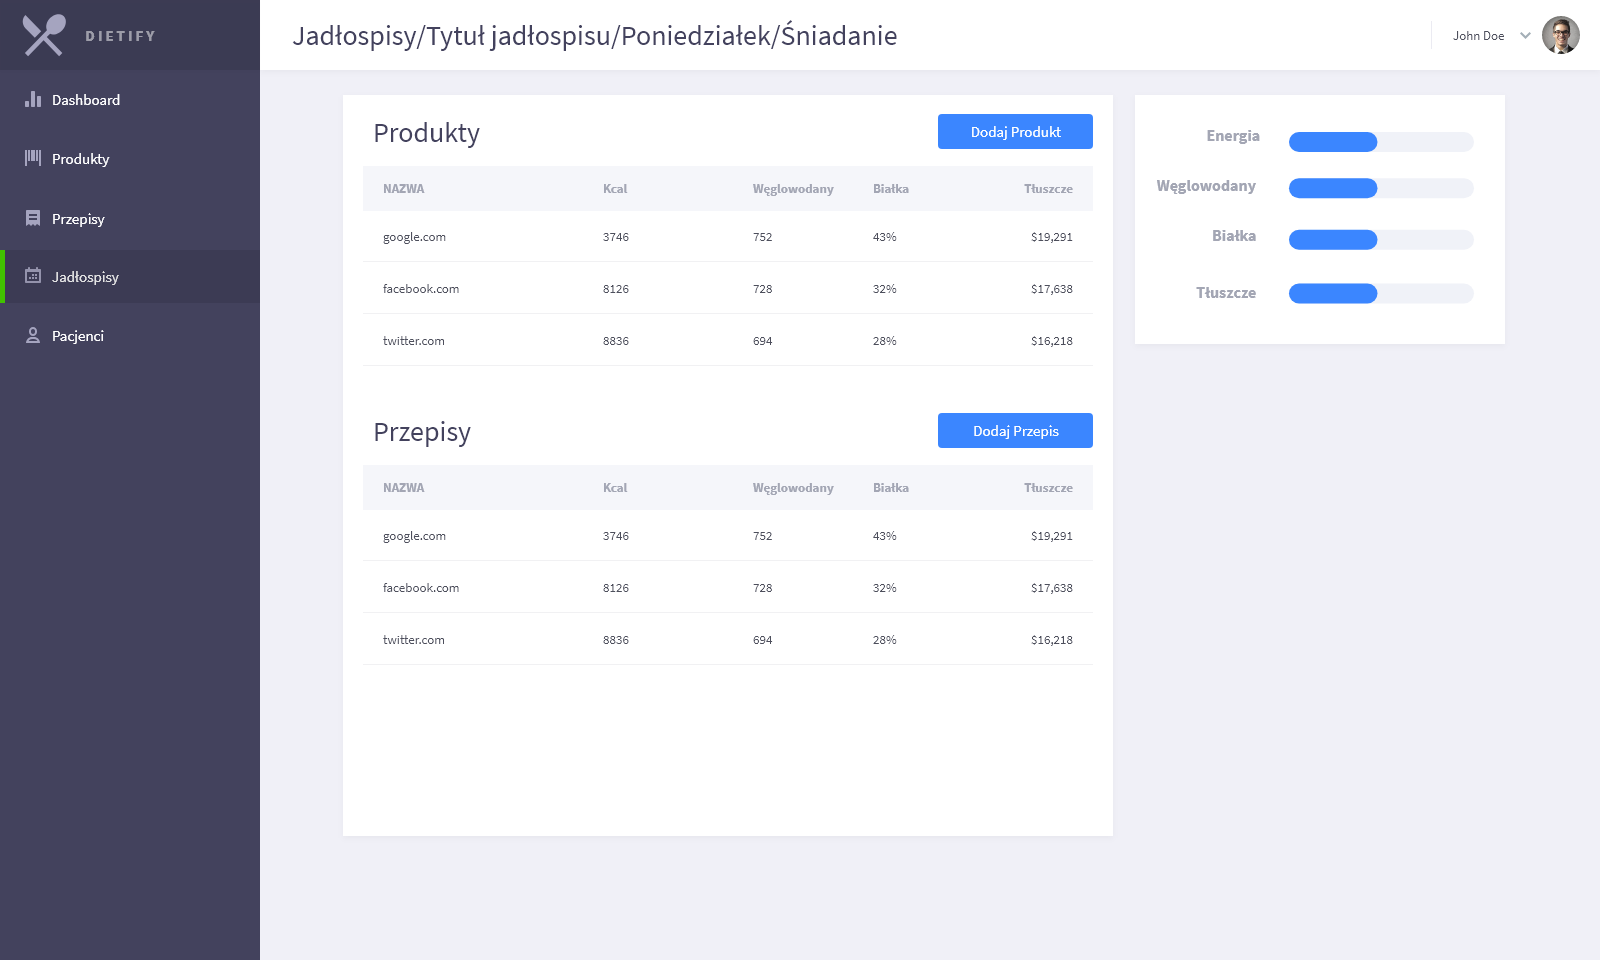
\includegraphics[width=0.9\textwidth]{img/mockups/mockup9.png}
        \caption{Mockup9 (opr.wł).}\label{rysunek:mockup9}
    \end{figure}
\end{minipage}

\begin{minipage}{\textwidth}
    \begin{figure}[H]
        \centering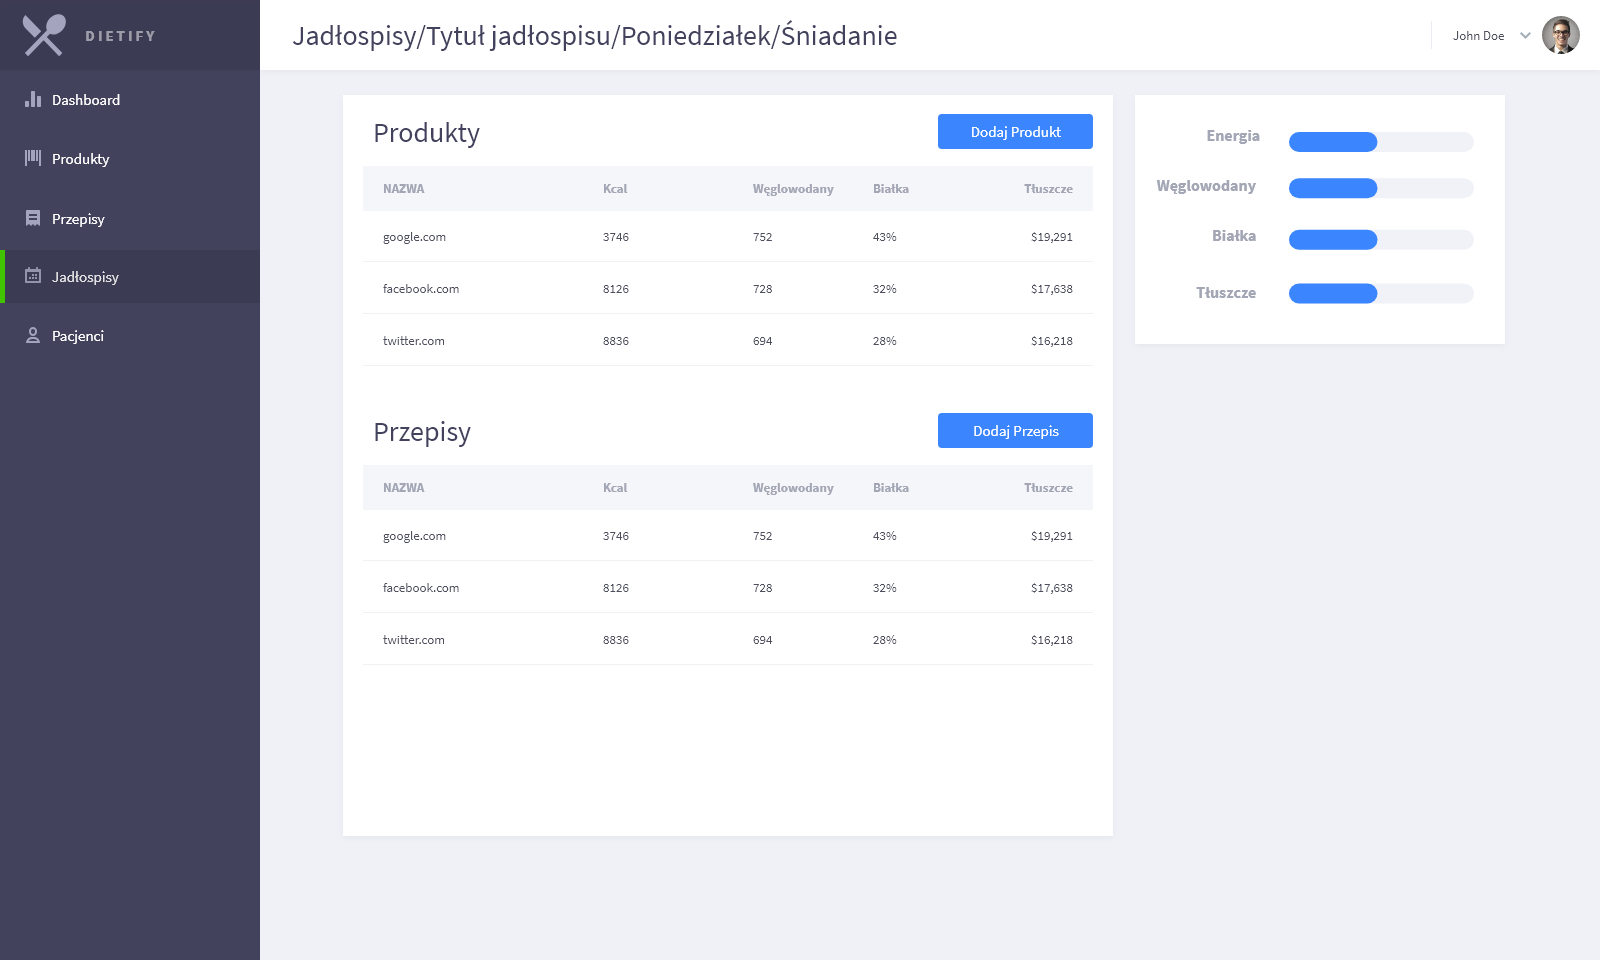
\includegraphics[width=0.9\textwidth]{img/mockups/mockup10.png}
        \caption{Mockup10 (opr.wł).}\label{rysunek:mockup10}
    \end{figure}
\end{minipage}

\begin{minipage}{\textwidth}
    \begin{figure}[H]
        \centering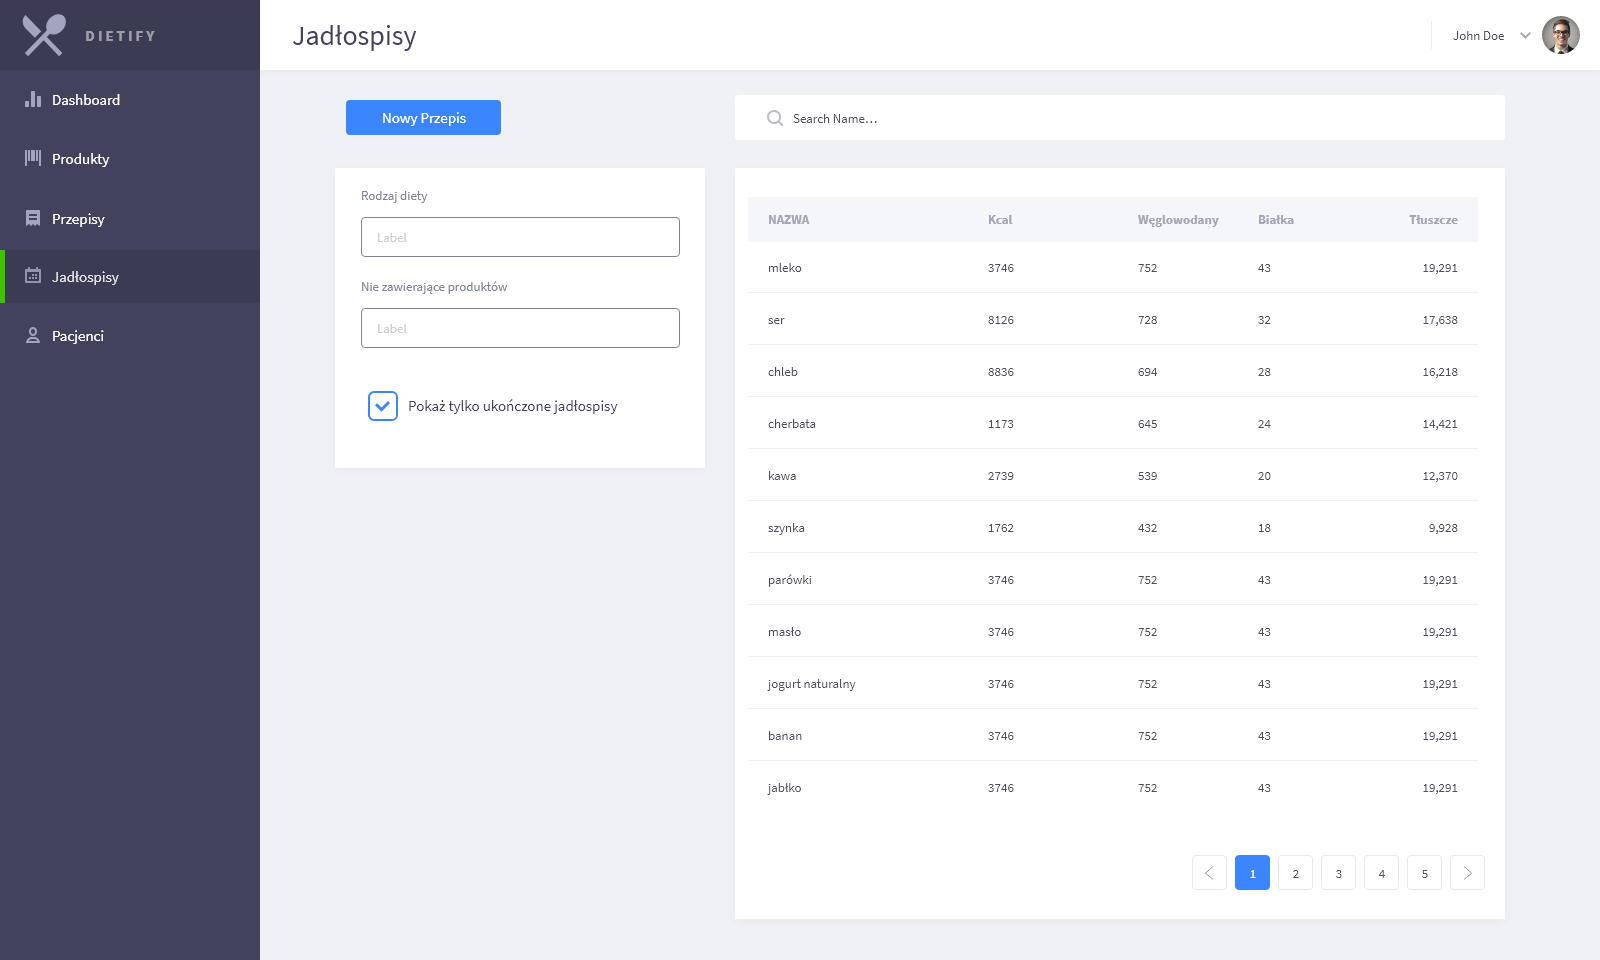
\includegraphics[width=0.9\textwidth]{img/mockups/mockup11.png}
        \caption{Mockup11 (opr.wł).}\label{rysunek:mockup11}
    \end{figure}
\end{minipage}

\begin{minipage}{\textwidth}
    \begin{figure}[H]
        \centering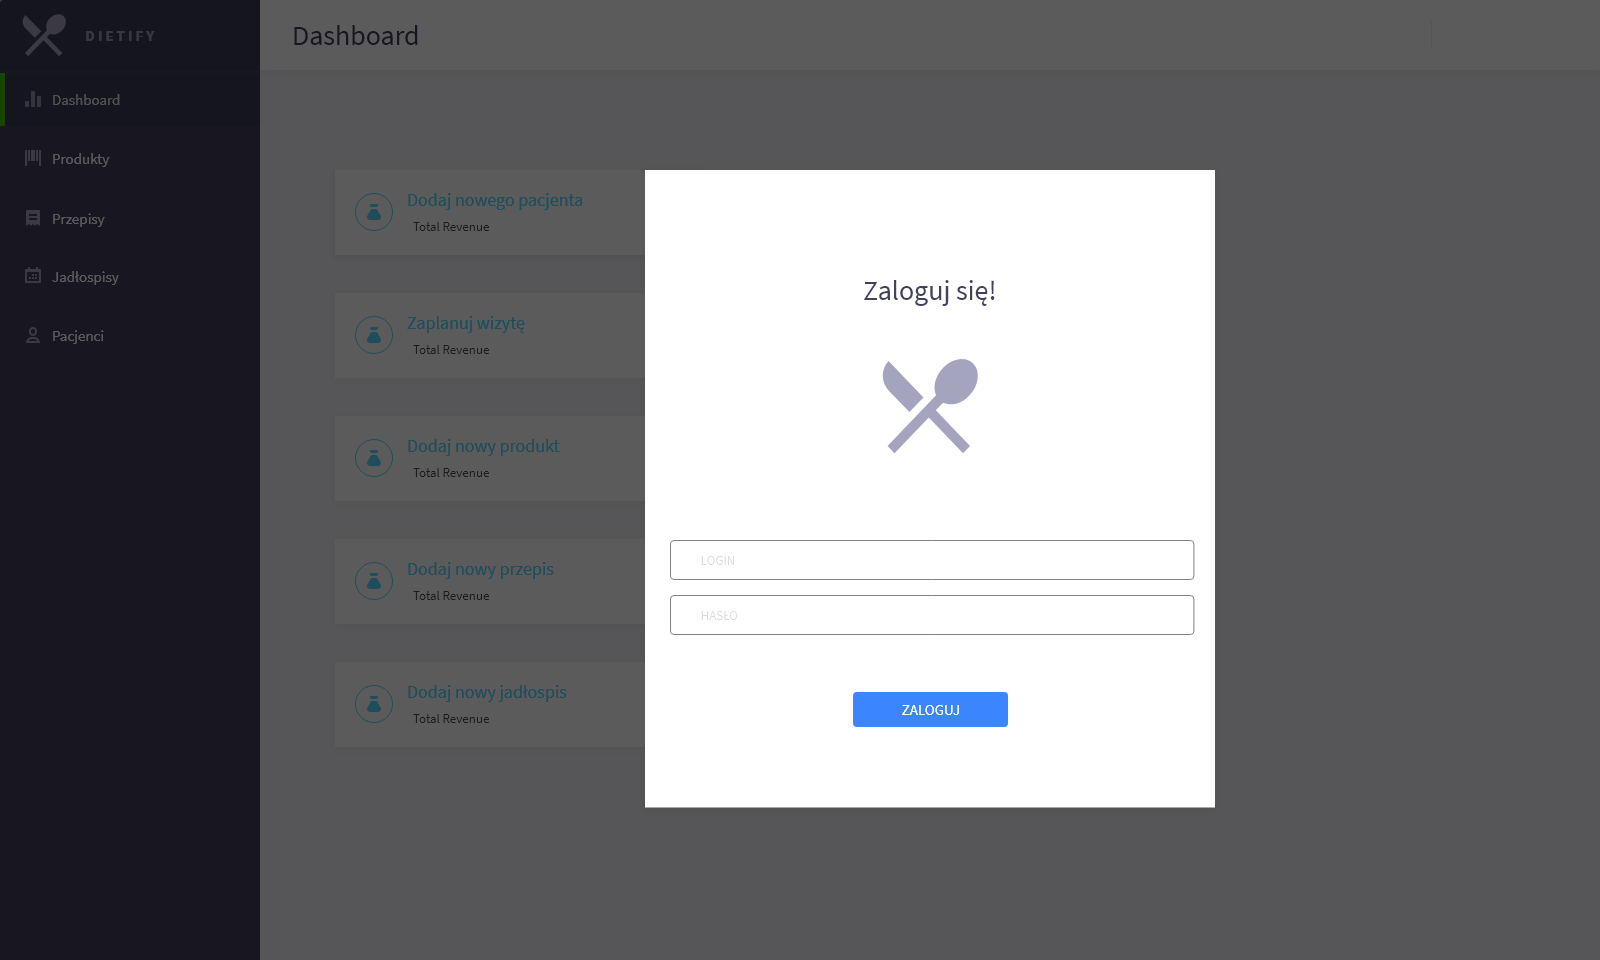
\includegraphics[width=0.9\textwidth]{img/mockups/mockup12.png}
        \caption{Mockup12 (opr.wł).}\label{rysunek:mockup12}
    \end{figure}
\end{minipage}

\begin{minipage}{\textwidth}
    \begin{figure}[H]
        \centering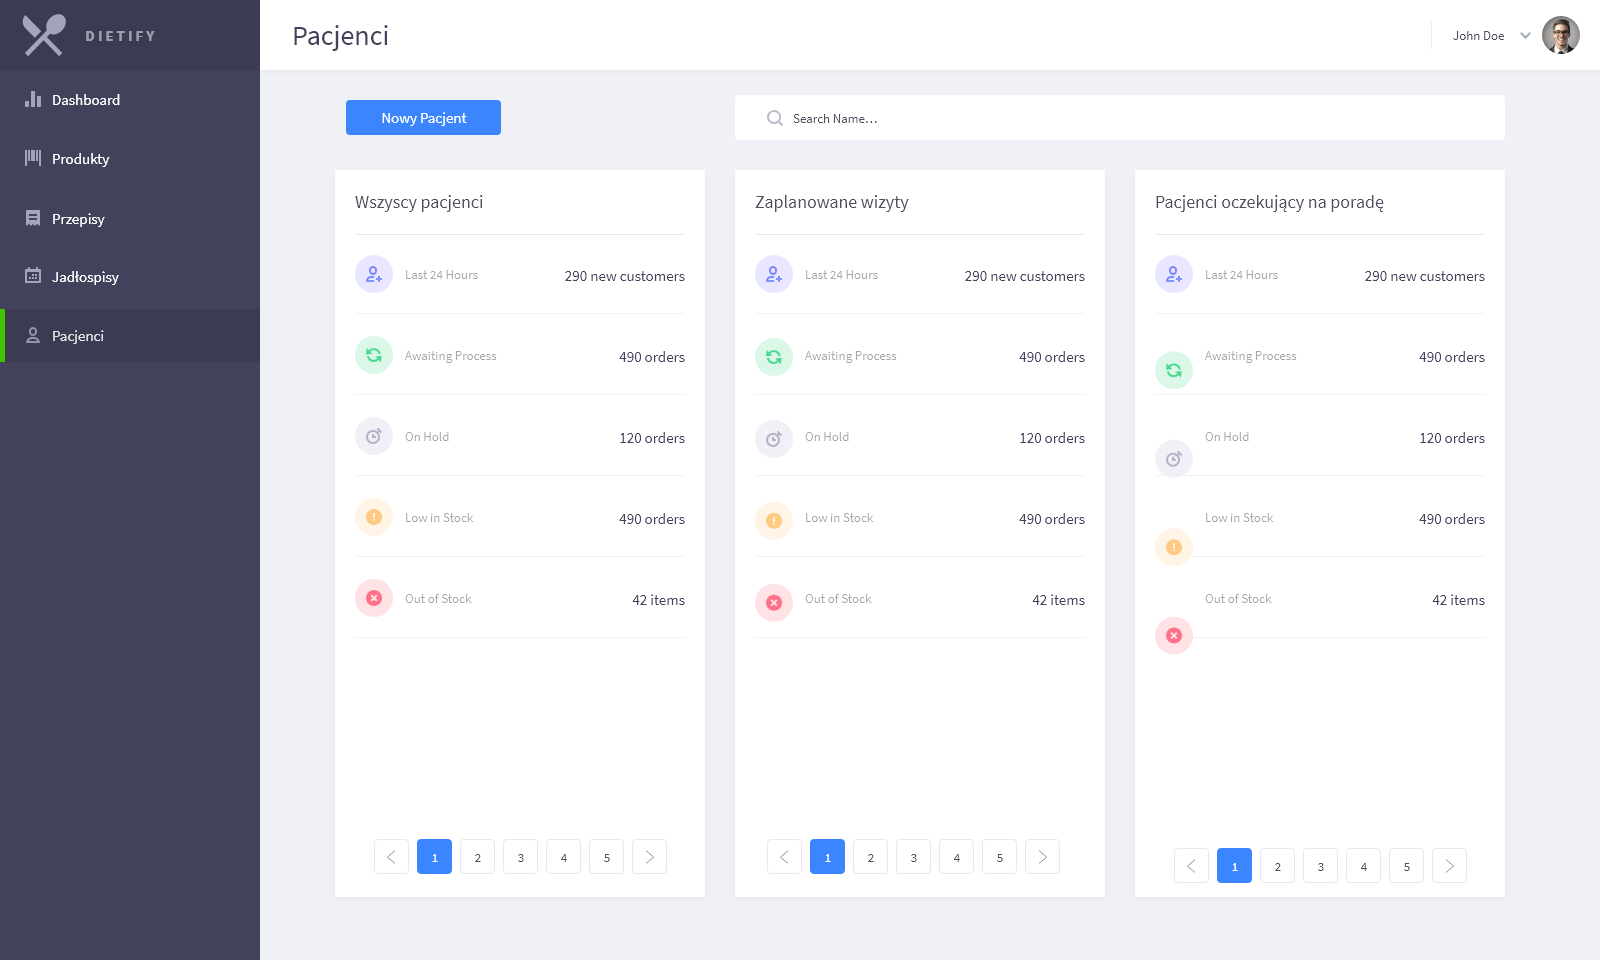
\includegraphics[width=0.9\textwidth]{img/mockups/mockup13.png}
        \caption{Mockup13 (opr.wł).}\label{rysunek:mockup13}
    \end{figure}
\end{minipage}

\begin{minipage}{\textwidth}
    \begin{figure}[H]
        \centering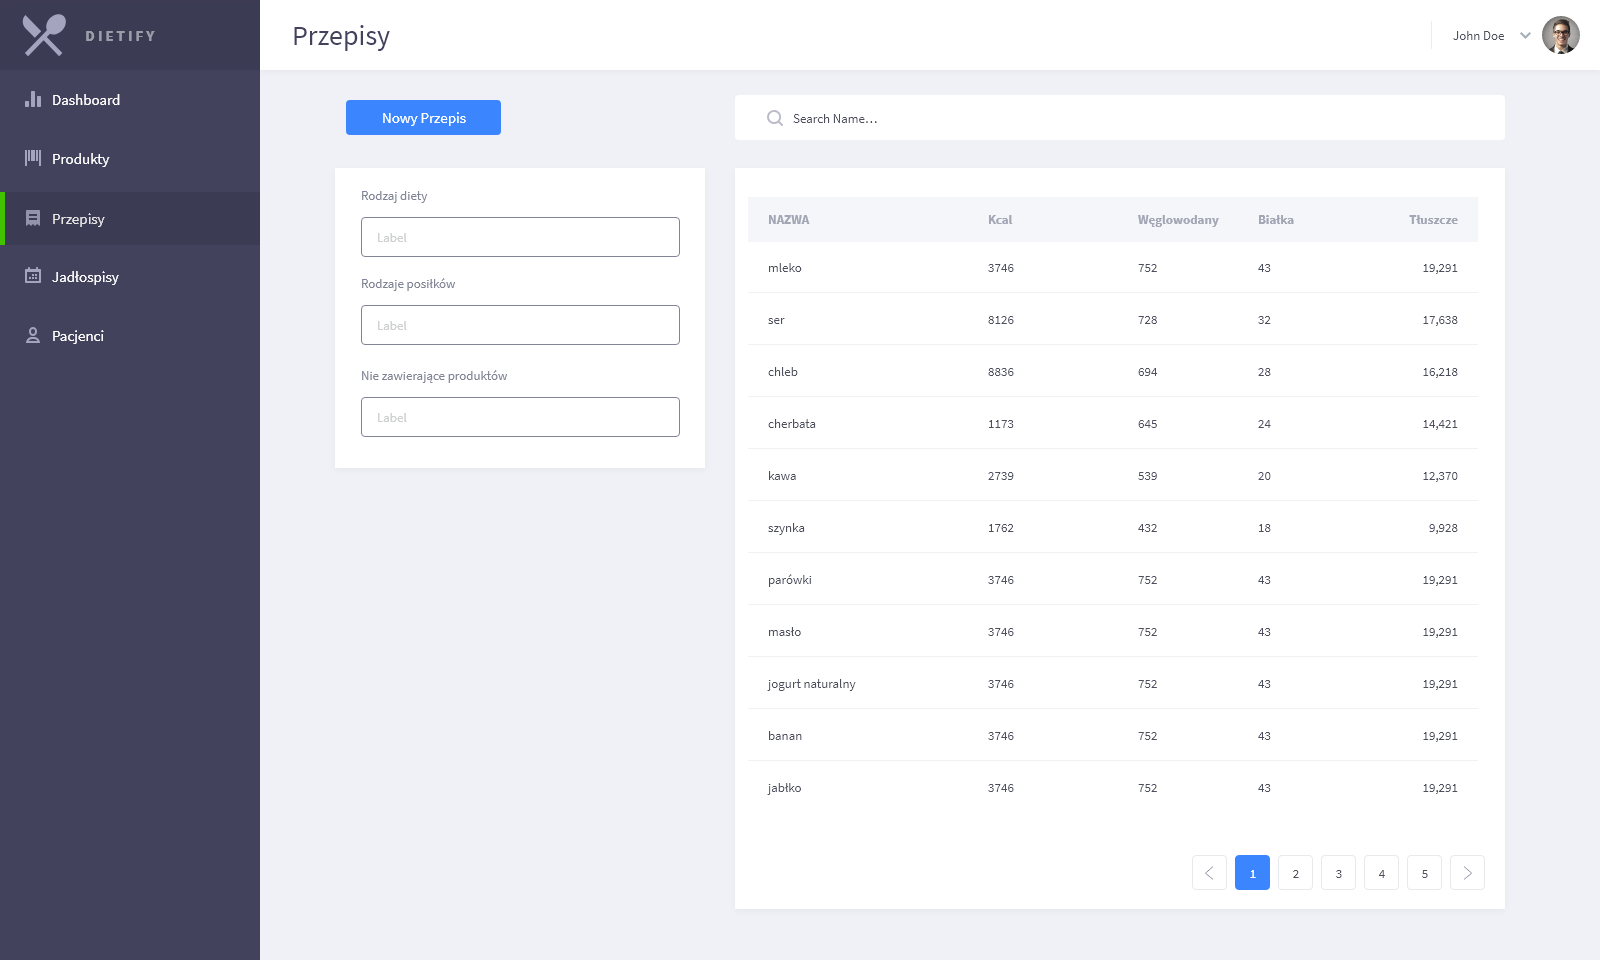
\includegraphics[width=0.9\textwidth]{img/mockups/mockup14.png}
        \caption{Mockup14 (opr.wł).}\label{rysunek:mockup14}
    \end{figure}
\end{minipage}

\begin{minipage}{\textwidth}
    \begin{figure}[H]
        \centering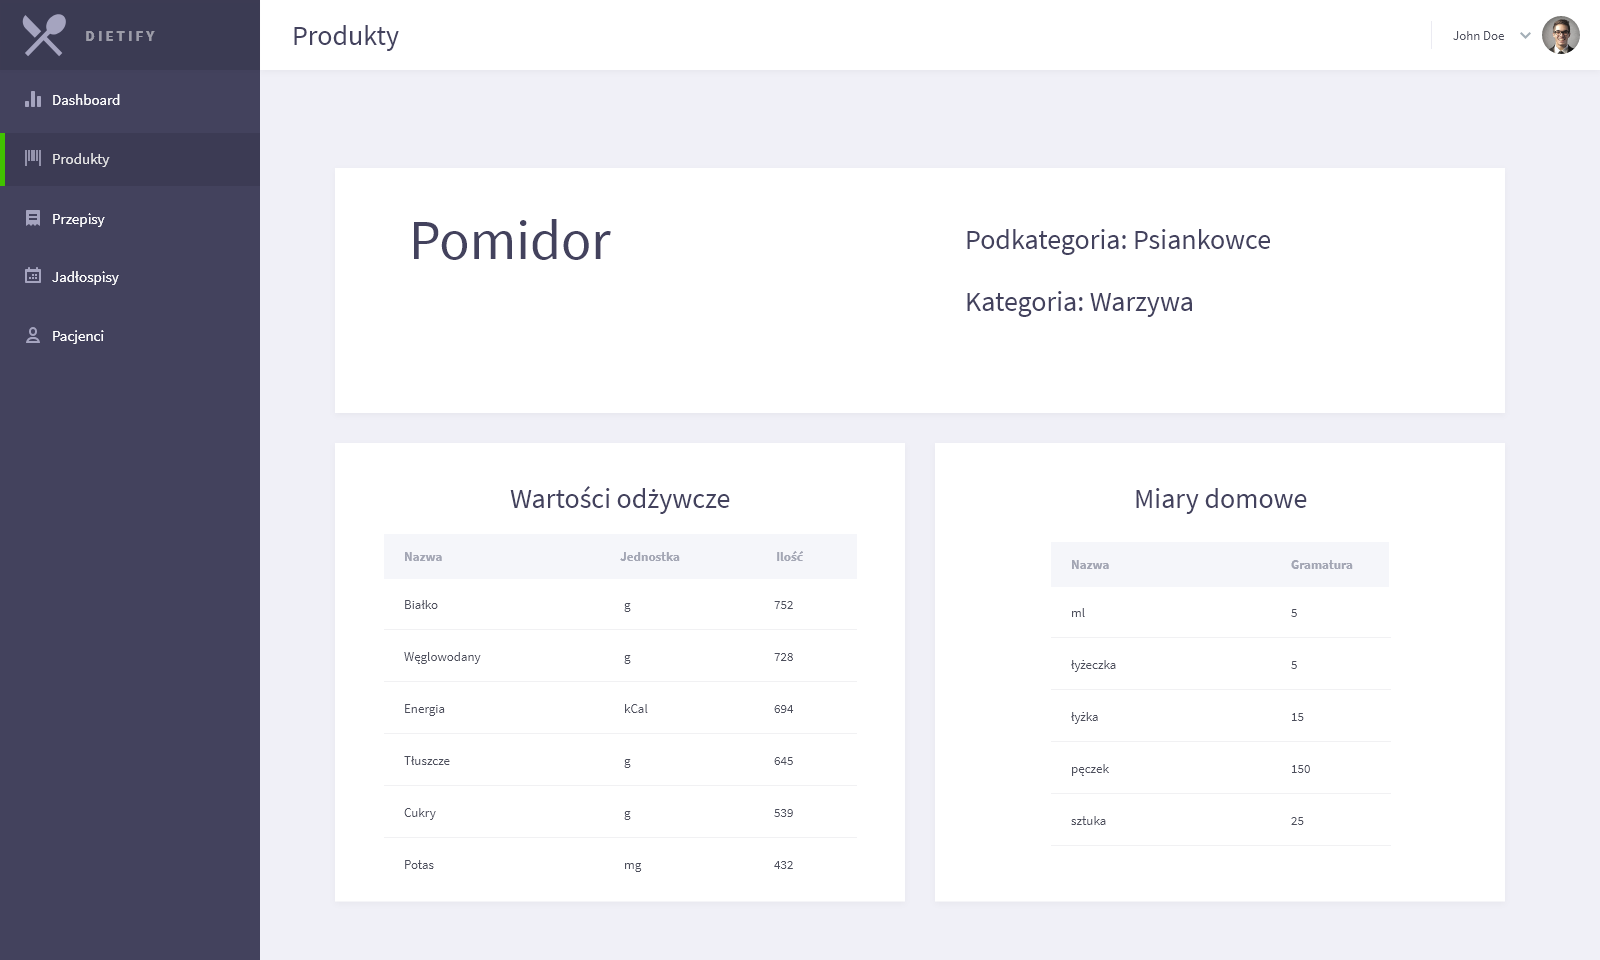
\includegraphics[width=0.9\textwidth]{img/mockups/mockup15.png}
        \caption{Mockup15 (opr.wł).}\label{rysunek:mockup15}
    \end{figure}
\end{minipage}

\begin{minipage}{\textwidth}
    \begin{figure}[H]
        \centering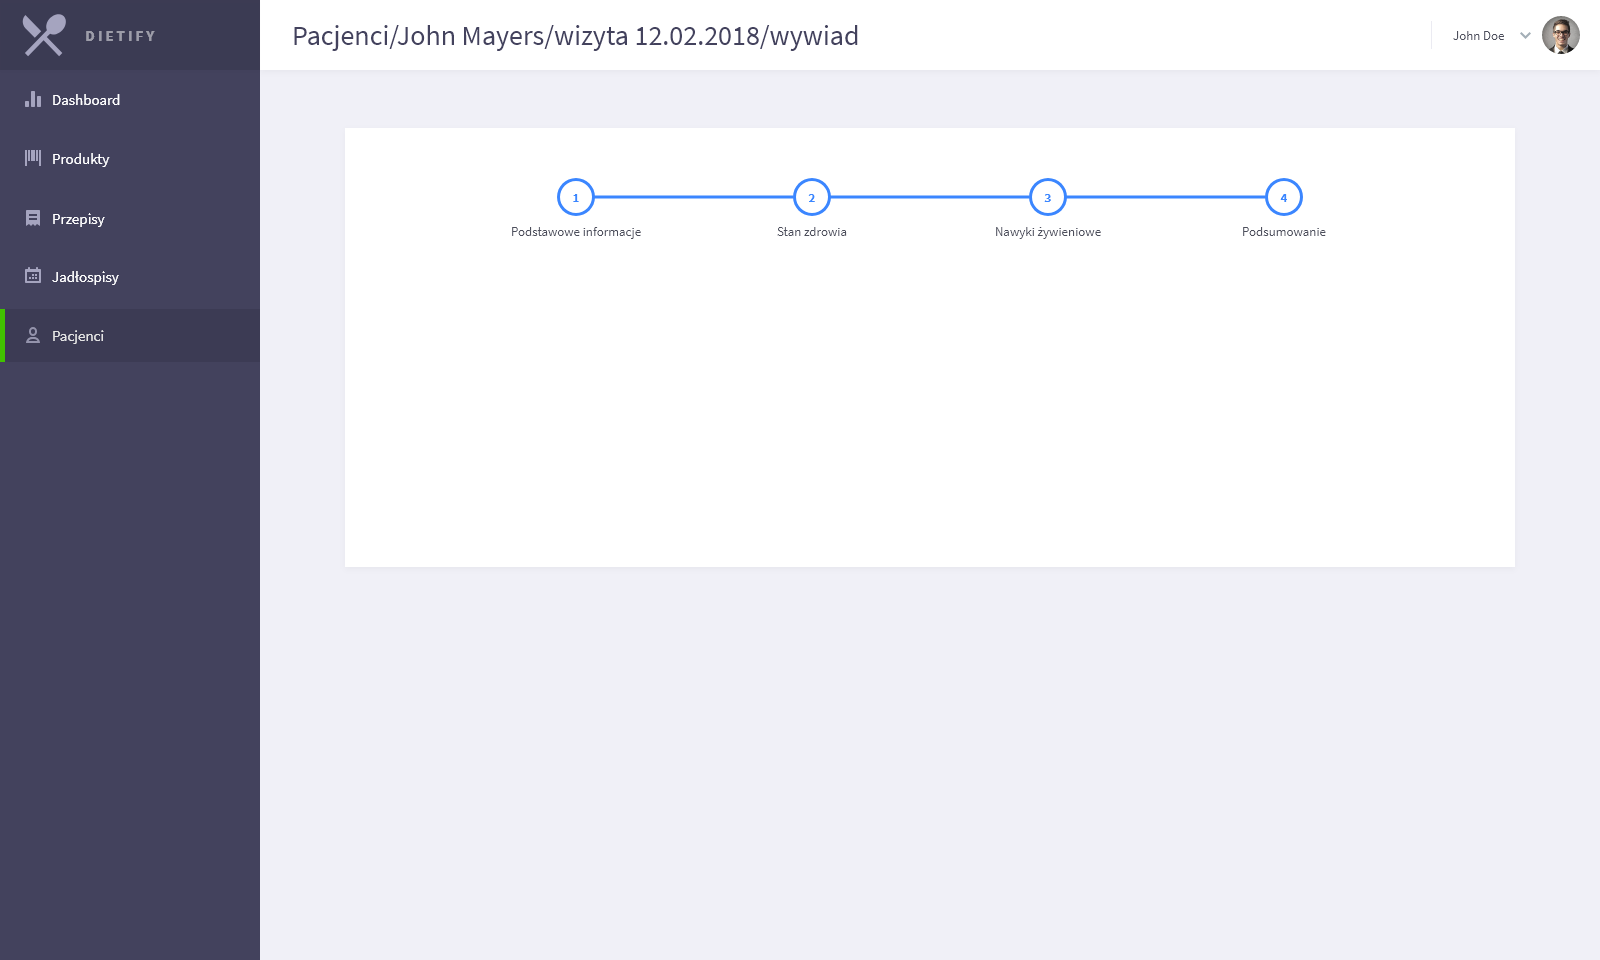
\includegraphics[width=0.9\textwidth]{img/mockups/mockup16.png}
        \caption{Mockup16 (opr.wł).}\label{rysunek:mockup16}
    \end{figure}
\end{minipage}

\section{Baza danych}

\subsection{Kategorie}
\todo{uzupełnić kategorie}

\begin{enumerate}[label={\textbf{KAT/\protect\threedigits{\theenumi}}}, wide, labelwidth=!, labelindent=0pt, labelsep=0pt, series=reqs]
    \setlength\itemsep{1em}
    \req{User} \label{kat:user} (Użytkownik)

    Opis: \lipsum[1]
    \par
    Atrybuty:
    \begin{itemize}[series=atr]
        \atr{id} \label{kat:user:id}
        \atr{login} \label{kat:user:login}
        \atr{passwordHash} \label{kat:user:passwordHash}
        \atr{firstName} \label{kat:user:firstName}
        \atr{lastName} \label{kat:user:lastName}
        \atr{email} \label{kat:user:email}
        \atr{image} \label{kat:user:image}
        \atr{activated} \label{kat:user:activated}
        \atr{langKey} \label{kat:user:langKey}
        \atr{activationKey} \label{kat:user:activationKey}
        \atr{createdBy} \label{kat:user:createdBy}
        \atr{createdDate} \label{kat:user:createdDate}
        \atr{resetDate} \label{kat:user:resetDate}
        \atr{lastModifiedBy} \label{kat:user:lastModifiedBy}
        \atr{lastModifiedDate} \label{kat:user:lastModifiedDate}
    \end{itemize}

    \req{Authority} \label{kat:authority} (Rola)

    Opis: \lipsum[1]
    \par
    Atrybuty:
    \begin{itemize}[series=atr]
        \atr{name} \label{kat:authority:name}
    \end{itemize}

    \req{UserExtraInfo} \label{kat:UserExtraInfo} (Dodatkowe Informacje Użytkownika)

    Opis: \lipsum[1]
    \par
    Atrybuty:
    \begin{itemize}[series=atr]
        \atr{id} \label{kat:UserExtraInfo:id}
        \atr{gender} \label{kat:UserExtraInfo:gender}
        \atr{dateOfBirth} \label{kat:UserExtraInfo:dateOfBirth}
        \atr{phoneNumber} \label{kat:UserExtraInfo:phoneNumber}
        \atr{streetAddress} \label{kat:UserExtraInfo:streetAddress}
        \atr{postalCode} \label{kat:UserExtraInfo:postalCode}
        \atr{city} \label{kat:UserExtraInfo:city}
        \atr{country} \label{kat:UserExtraInfo:country}
        \atr{personalDescription} \label{kat:UserExtraInfo:personalDescription}
    \end{itemize}

    \req{SiteContent} \label{kat:SiteContent} (Treść Strony)

    Opis: \lipsum[1]
    \par
    Atrybuty:
    \begin{itemize}[series=atr]
        \atr{id} \label{kat:SiteContent:id}
        \atr{ordinalNumber} \label{kat:SiteContent:ordinalNumber}
        \atr{siteContentType} \label{kat:SiteContent:siteContentType}
        \atr{title} \label{kat:SiteContent:title}
        \atr{description} \label{kat:SiteContent:description}
    \end{itemize}

    \req{SiteContentTranslation} \label{kat:SiteContentTranslation} (Tłumaczenie Treści Strony)

    Opis: \lipsum[1]
    \par
    Atrybuty:
    \begin{itemize}[series=atr]
        \atr{id} \label{kat:SiteContentTranslation:id}
        \atr{title} \label{kat:SiteContentTranslation:title}
        \atr{description} \label{kat:SiteContentTranslation:description}
        \atr{language} \label{kat:SiteContentTranslation:language}
    \end{itemize}

    \req{ContactInfo} \label{kat:ContactInfo} (Informacje Kontaktowe)

    Opis: \lipsum[1]
    \par
    Atrybuty:
    \begin{itemize}[series=atr]
        \atr{id} \label{kat:ContactInfo:id}
        \atr{contactInfoType} \label{kat:ContactInfo:contactInfoType}
        \atr{description} \label{kat:ContactInfo:description}
    \end{itemize}

    \req{Pricing} \label{kat:Pricing} (Cennik)

    Opis: \lipsum[1]
    \par
    Atrybuty:
    \begin{itemize}[series=atr]
        \atr{id} \label{kat:Pricing:id}
        \atr{ordinalNumber} \label{kat:Pricing:ordinalNumber}
        \atr{title} \label{kat:Pricing:title}
        \atr{description} \label{kat:Pricing:description}
        \atr{price} \label{kat:Pricing:price}
        \atr{currency} \label{kat:Pricing:currency}
    \end{itemize}

    \req{PricingTranslation} \label{kat:PricingTranslation} (Tłumaczenie Cennika)

    Opis: \lipsum[1]
    \par
    Atrybuty:
    \begin{itemize}[series=atr]
        \atr{id} \label{kat:PricingTranslation:id}
        \atr{title} \label{kat:PricingTranslation:title}
        \atr{description} \label{kat:PricingTranslation:description}
        \atr{language} \label{kat:PricingTranslation:language}
    \end{itemize}

    \req{Product} \label{kat:Product} (Produkt)

    Opis: \lipsum[1]
    \par
    Atrybuty:
    \begin{itemize}[series=atr]
        \atr{id} \label{kat:Product:id}
        \atr{source} \label{kat:Product:source}
        \atr{isPublic} \label{kat:Product:isPublic}
        \atr{language} \label{kat:Product:language}
    \end{itemize}

    \req{ProductVersion} \label{kat:ProductVersion} (Wersja Produktu)

    Opis: \lipsum[1]
    \par
    Atrybuty:
    \begin{itemize}[series=atr]
        \atr{id} \label{kat:ProductVersion:id}
        \atr{editTimestamp} \label{kat:ProductVersion:editTimestamp}
        \atr{description} \label{kat:ProductVersion:description}
    \end{itemize}

    \req{ProductBasicNutritionData} \label{kat:ProductBasicNutritionData} (Podstawowe Składniki Odżywcze Produktu)

    Opis: \lipsum[1]
    \par
    Atrybuty:
    \begin{itemize}[series=atr]
        \atr{id} \label{kat:ProductBasicNutritionData:id}
        \atr{energy} \label{kat:ProductBasicNutritionData:energy}
        \atr{protein} \label{kat:ProductBasicNutritionData:protein}
        \atr{fat} \label{kat:ProductBasicNutritionData:fat}
        \atr{carbohydrates} \label{kat:ProductBasicNutritionData:carbohydrates}
    \end{itemize}

    \req{NutritionData} \label{kat:NutritionData} (Wartość Odżywcza)

    Opis: \lipsum[1]
    \par
    Atrybuty:
    \begin{itemize}[series=atr]
        \atr{id} \label{kat:NutritionData:id}
        \atr{nutritionValue} \label{kat:NutritionData:nutritionValue}
    \end{itemize}

    \req{NutritionDefinition} \label{kat:NutritionDefinition} (Definicja Wartości Odżywczej)

    Opis: \lipsum[1]
    \par
    Atrybuty:
    \begin{itemize}[series=atr]
        \atr{id} \label{kat:NutritionDefinition:id}
        \atr{tag} \label{kat:NutritionDefinition:tag}
        \atr{description} \label{kat:NutritionDefinition:description}
        \atr{units} \label{kat:NutritionDefinition:units}
        \atr{decimalPlaces} \label{kat:NutritionDefinition:decimalPlaces}
    \end{itemize}

    \req{NutritionDefinitionTranslation} \label{kat:NutritionDefinitionTranslation} (Tłumaczenie Definicji Wartości Odżywczej)

    Opis: \lipsum[1]
    \par
    Atrybuty:
    \begin{itemize}[series=atr]
        \atr{id} \label{kat:NutritionDefinitionTranslation:id}
        \atr{translation} \label{kat:NutritionDefinitionTranslation:translation}
        \atr{language} \label{kat:NutritionDefinitionTranslation:language}
    \end{itemize}

    \req{HouseholdMeasure} \label{kat:HouseholdMeasure} (Miara Domowa)

    Opis: \lipsum[1]
    \par
    Atrybuty:
    \begin{itemize}[series=atr]
        \atr{id} \label{kat:HouseholdMeasure:id}
        \atr{description} \label{kat:HouseholdMeasure:description}
        \atr{gramsWeight} \label{kat:HouseholdMeasure:gramsWeight}
        \atr{isVisible} \label{kat:HouseholdMeasure:isVisible}
    \end{itemize}

    \req{ProductSubcategory} \label{kat:ProductSubcategory} (Podkategoria Produktu)

    Opis: \lipsum[1]
    \par
    Atrybuty:
    \begin{itemize}[series=atr]
        \atr{id} \label{kat:ProductSubcategory:id}
        \atr{description} \label{kat:ProductSubcategory:description}
    \end{itemize}

    \req{ProductCategory} \label{kat:ProductCategory} (Kategoria Produktu)

    Opis: \lipsum[1]
    \par
    Atrybuty:
    \begin{itemize}[series=atr]
        \atr{id} \label{kat:ProductCategory:id}
        \atr{description} \label{kat:ProductCategory:description}
    \end{itemize}

    \req{ProductCategoryTranslation} \label{kat:ProductCategoryTranslation} (Tłumaczenie Kategorii Produktu)

    Opis: \lipsum[1]
    \par
    Atrybuty:
    \begin{itemize}[series=atr]
        \atr{id} \label{kat:ProductCategoryTranslation:id}
        \atr{translation} \label{kat:ProductCategoryTranslation:translation}
        \atr{language} \label{kat:ProductCategoryTranslation:language}
    \end{itemize}

    \req{DietType} \label{kat:DietType} (Typ Diety)

    Opis: \lipsum[1]
    \par
    Atrybuty:
    \begin{itemize}[series=atr]
        \atr{id} \label{kat:DietType:id}
        \atr{name} \label{kat:DietType:name}
    \end{itemize}

    \req{DietTypeTranslation} \label{kat:DietTypeTranslation} (Tłumaczenie Typu Diety)

    Opis: \lipsum[1]
    \par
    Atrybuty:
    \begin{itemize}[series=atr]
        \atr{id} \label{kat:DietTypeTranslation:id}
        \atr{translation} \label{kat:DietTypeTranslation:translation}
        \atr{language} \label{kat:DietTypeTranslation:language}
    \end{itemize}

    \req{Recipe} \label{kat:Recipe} (Przepis)

    Opis: \lipsum[1]
    \par
    Atrybuty:
    \begin{itemize}[series=atr]
        \atr{id} \label{kat:Recipe:id}
        \atr{isPublic} \label{kat:Recipe:isPublic}
        \atr{language} \label{kat:Recipe:language}
    \end{itemize}

    \req{RecipeVersion} \label{kat:RecipeVersion} (Wersja Przepisu)

    Opis: \lipsum[1]
    \par
    Atrybuty:
    \begin{itemize}[series=atr]
        \atr{id} \label{kat:RecipeVersion:id}
        \atr{editTimestamp} \label{kat:RecipeVersion:editTimestamp}
        \atr{name} \label{kat:RecipeVersion:name}
        \atr{preparationTimeMinutes} \label{kat:RecipeVersion:preparationTimeMinutes}
        \atr{numberOfPortions} \label{kat:RecipeVersion:numberOfPortions}
        \atr{image} \label{kat:RecipeVersion:image}
        \atr{totalGramsWeight} \label{kat:RecipeVersion:totalGramsWeight}
    \end{itemize}

    \req{RecipeBasicNutritionData} \label{kat:RecipeBasicNutritionData} (Podstawowe Wartości Odżywcze Przepisu)

    Opis: \lipsum[1]
    \par
    Atrybuty:
    \begin{itemize}[series=atr]
        \atr{id} \label{kat:RecipeBasicNutritionData:id}
        \atr{energy} \label{kat:RecipeBasicNutritionData:energy}
        \atr{protein} \label{kat:RecipeBasicNutritionData:protein}
        \atr{fat} \label{kat:RecipeBasicNutritionData:fat}
        \atr{carbohydrates} \label{kat:RecipeBasicNutritionData:carbohydrates}
    \end{itemize}

    \req{RecipeSection} \label{kat:RecipeSection} (Sekcja Przepisu)

    Opis: \lipsum[1]
    \par
    Atrybuty:
    \begin{itemize}[series=atr]
        \atr{id} \label{kat:RecipeSection:id}
        \atr{sectionName} \label{kat:RecipeSection:sectionName}
    \end{itemize}

    \req{ProductPortion} \label{kat:ProductPortion} (Porcja Produktu)

    Opis: \lipsum[1]
    \par
    Atrybuty:
    \begin{itemize}[series=atr]
        \atr{id} \label{kat:ProductPortion:id}
        \atr{amount} \label{kat:ProductPortion:amount}
    \end{itemize}

    \req{PreparationStep} \label{kat:PreparationStep} (Krok Przygotowania)

    Opis: \lipsum[1]
    \par
    Atrybuty:
    \begin{itemize}[series=atr]
        \atr{id} \label{kat:PreparationStep:id}
        \atr{ordinalNumber} \label{kat:PreparationStep:ordinalNumber}
        \atr{stepDescription} \label{kat:PreparationStep:stepDescription}
    \end{itemize}

    \req{KitchenAppliance} \label{kat:KitchenAppliance} (Wyposażenie Kuchenne)

    Opis: \lipsum[1]
    \par
    Atrybuty:
    \begin{itemize}[series=atr]
        \atr{id} \label{kat:KitchenAppliance:id}
        \atr{name} \label{kat:KitchenAppliance:name}
    \end{itemize}

    \req{KitchenApplianceTranslation} \label{kat:KitchenApplianceTranslation} (Tłumaczenie Wyposażenia Kuchennego)

    Opis: \lipsum[1]
    \par
    Atrybuty:
    \begin{itemize}[series=atr]
        \atr{id} \label{kat:KitchenApplianceTranslation:id}
        \atr{translation} \label{kat:KitchenApplianceTranslation:translation}
        \atr{language} \label{kat:KitchenApplianceTranslation:language}
    \end{itemize}

    \req{DishType} \label{kat:DishType} (Typ Dania)

    Opis: \lipsum[1]
    \par
    Atrybuty:
    \begin{itemize}[series=atr]
        \atr{id} \label{kat:DishType:id}
        \atr{description} \label{kat:DishType:description}
    \end{itemize}

    \req{DishTypeTranslation} \label{kat:DishTypeTranslation} (Tłumaczenie Typu Dania)

    Opis: \lipsum[1]
    \par
    Atrybuty:
    \begin{itemize}[series=atr]
        \atr{id} \label{kat:DishTypeTranslation:id}
        \atr{translation} \label{kat:DishTypeTranslation:translation}
        \atr{language} \label{kat:DishTypeTranslation:language}
    \end{itemize}

    \req{MealType} \label{kat:MealType} (Typ Posiłku)

    Opis: \lipsum[1]
    \par
    Atrybuty:
    \begin{itemize}[series=atr]
        \atr{id} \label{kat:MealType:id}
        \atr{name} \label{kat:MealType:name}
    \end{itemize}

    \req{MealTypeTranslation} \label{kat:MealTypeTranslation} (Tłumaczenie Typu Posiłku)

    Opis: \lipsum[1]
    \par
    Atrybuty:
    \begin{itemize}[series=atr]
        \atr{id} \label{kat:MealTypeTranslation:id}
        \atr{translation} \label{kat:MealTypeTranslation:translation}
        \atr{language} \label{kat:MealTypeTranslation:language}
    \end{itemize}


    \req{MealPlan} \label{kat:MealPlan} (Jadłospis)

    Opis: \lipsum[1]
    \par
    Atrybuty:
    \begin{itemize}[series=atr]
        \atr{id} \label{kat:MealPlan:id}
        \atr{creationTimestamp} \label{kat:MealPlan:creationTimestamp}
        \atr{editTimestamp} \label{kat:MealPlan:editTimestamp}
        \atr{name} \label{kat:MealPlan:name}
        \atr{isVisible} \label{kat:MealPlan:isVisible}
        \atr{language} \label{kat:MealPlan:language}
        \atr{numberOfDays} \label{kat:MealPlan:numberOfDays}
        \atr{numberOfMealsPerDay} \label{kat:MealPlan:numberOfMealsPerDay}
        \atr{totalDailyEnergy} \label{kat:MealPlan:totalDailyEnergy}
        \atr{percentOfProtein} \label{kat:MealPlan:percentOfProtein}
        \atr{percentOfFat} \label{kat:MealPlan:percentOfFat}
        \atr{percentOfCarbohydrates} \label{kat:MealPlan:percentOfCarbohydrates}
    \end{itemize}

    \req{MealPlanDay} \label{kat:MealPlanDay} (Dzień Jadłospisu)

    Opis: \lipsum[1]
    \par
    Atrybuty:
    \begin{itemize}[series=atr]
        \atr{id} \label{kat:MealPlanDay:id}
        \atr{ordinalNumber} \label{kat:MealPlanDay:ordinalNumber}
    \end{itemize}

    \req{Meal} \label{kat:Meal} (Posiłek)

    Opis: \lipsum[1]
    \par
    Atrybuty:
    \begin{itemize}[series=atr]
        \atr{id} \label{kat:Meal:id}
        \atr{ordinalNumber} \label{kat:Meal:ordinalNumber}
    \end{itemize}

    \req{MealRecipe} \label{kat:MealRecipe} (Przepis Posiłku)

    Opis: \lipsum[1]
    \par
    Atrybuty:
    \begin{itemize}[series=atr]
        \atr{id} \label{kat:MealRecipe:id}
        \atr{amount} \label{kat:MealRecipe:amount}
    \end{itemize}

    \req{MealProduct} \label{kat:MealProduct} (Produkt Posiłku)

    Opis: \lipsum[1]
    \par
    Atrybuty:
    \begin{itemize}[series=atr]
        \atr{id} \label{kat:MealProduct:id}
        \atr{amount} \label{kat:MealProduct:amount}
    \end{itemize}

    \req{MealDefinition} \label{kat:MealDefinition} (Definicja Posiłku)

    Opis: \lipsum[1]
    \par
    Atrybuty:
    \begin{itemize}[series=atr]
        \atr{id} \label{kat:MealDefinition:id}
        \atr{ordinalNumber} \label{kat:MealDefinition:ordinalNumber}
        \atr{timeOfMeal} \label{kat:MealDefinition:timeOfMeal}
        \atr{percentOfEnergy} \label{kat:MealDefinition:percentOfEnergy}
    \end{itemize}

    \req{Appointment} \label{kat:Appointment} (Wizyta)

    Opis: \lipsum[1]
    \par
    Atrybuty:
    \begin{itemize}[series=atr]
        \atr{id} \label{kat:Appointment:id}
        \atr{appointmentDate} \label{kat:Appointment:appointmentDate}
        \atr{appointmentState} \label{kat:Appointment:appointmentState}
        \atr{generalAdvice} \label{kat:Appointment:generalAdvice}
    \end{itemize}

    \req{PatientCard} \label{kat:PatientCard} (Karta Pacjenta)

    Opis: \lipsum[1]
    \par
    Atrybuty:
    \begin{itemize}[series=atr]
        \atr{id} \label{kat:PatientCard:id}
        \atr{creationDate} \label{kat:PatientCard:creationDate}
    \end{itemize}

    \req{AppointmentEvaluation} \label{kat:AppointmentEvaluation} (Ewaluacja Wizyty)

    Opis: \lipsum[1]
    \par
    Atrybuty:
    \begin{itemize}[series=atr]
        \atr{id} \label{kat:AppointmentEvaluation:id}
        \atr{overallSatisfaction} \label{kat:AppointmentEvaluation:overallSatisfaction}
        \atr{dietitianServiceSatisfaction} \label{kat:AppointmentEvaluation:dietitianServiceSatisfaction}
        \atr{mealPlanOverallSatisfaction} \label{kat:AppointmentEvaluation:mealPlanOverallSatisfaction}
        \atr{mealCostSatisfaction} \label{kat:AppointmentEvaluation:mealCostSatisfaction}
        \atr{mealPreparationTimeSatisfaction} \label{kat:AppointmentEvaluation:mealPreparationTimeSatisfaction}
        \atr{mealComplexityLevelSatisfaction} \label{kat:AppointmentEvaluation:mealComplexityLevelSatisfaction}
        \atr{mealTastefulnessSatisfaction} \label{kat:AppointmentEvaluation:mealTastefulnessSatisfaction}
        \atr{dietaryResultSatisfaction} \label{kat:AppointmentEvaluation:dietaryResultSatisfaction}
        \atr{comment} \label{kat:AppointmentEvaluation:comment}
    \end{itemize}

    \req{BodyMeasurement} \label{kat:BodyMeasurement} (Pomiar Ciała)

    Opis: \lipsum[1]
    \par
    Atrybuty:
    \begin{itemize}[series=atr]
        \atr{id} \label{kat:BodyMeasurement:id}
        \atr{completionDate} \label{kat:BodyMeasurement:completionDate}
        \atr{height} \label{kat:BodyMeasurement:height}
        \atr{weight} \label{kat:BodyMeasurement:weight}
        \atr{waist} \label{kat:BodyMeasurement:waist}
        \atr{percentOfFatTissue} \label{kat:BodyMeasurement:percentOfFatTissue}
        \atr{percentOfWater} \label{kat:BodyMeasurement:percentOfWater}
        \atr{muscleMass} \label{kat:BodyMeasurement:muscleMass}
        \atr{physicalMark} \label{kat:BodyMeasurement:physicalMark}
        \atr{calciumInBones} \label{kat:BodyMeasurement:calciumInBones}
        \atr{basicMetabolism} \label{kat:BodyMeasurement:basicMetabolism}
        \atr{metabolicAge} \label{kat:BodyMeasurement:metabolicAge}
        \atr{visceralDatLevel} \label{kat:BodyMeasurement:visceralDatLevel}
    \end{itemize}

    \req{NutritionalInterview} \label{kat:NutritionalInterview} (Wywiad Żywieniowy)

    Opis: \lipsum[1]
    \par
    Atrybuty:
    \begin{itemize}[series=atr]
        \atr{id} \label{kat:NutritionalInterview:id}
        \atr{completionDate} \label{kat:NutritionalInterview:completionDate}
        \atr{targetWeight} \label{kat:NutritionalInterview:targetWeight}
        \atr{advicePurpose} \label{kat:NutritionalInterview:advicePurpose}
        \atr{physicalActivity} \label{kat:NutritionalInterview:physicalActivity}
        \atr{diseases} \label{kat:NutritionalInterview:diseases}
        \atr{medicines} \label{kat:NutritionalInterview:medicines}
        \atr{jobType} \label{kat:NutritionalInterview:jobType}
        \atr{likedProducts} \label{kat:NutritionalInterview:likedProducts}
        \atr{dislikedProducts} \label{kat:NutritionalInterview:dislikedProducts}
        \atr{foodAllergies} \label{kat:NutritionalInterview:foodAllergies}
        \atr{foodIntolerances} \label{kat:NutritionalInterview:foodIntolerances}
    \end{itemize}

    \req{CustomNutritionalInterviewQuestion} \label{kat:CustomNutritionalInterviewQuestion} (Niestandardowe Pytanie Wywiadu Żywieniowego)

    Opis: \lipsum[1]
    \par
    Atrybuty:
    \begin{itemize}[series=atr]
        \atr{id} \label{kat:CustomNutritionalInterviewQuestion:id}
        \atr{ordinalNumber} \label{kat:CustomNutritionalInterviewQuestion:ordinalNumber}
        \atr{question} \label{kat:CustomNutritionalInterviewQuestion:question}
        \atr{answer} \label{kat:CustomNutritionalInterviewQuestion:answer}
    \end{itemize}

    \req{CustomNutritionalInterviewQuestionTemplate} \label{kat:CustomNutritionalInterviewQuestionTemplate} (Szablon Niestandardowego Pytania Wywiadu Żywieniowego)

    Opis: \lipsum[1]
    \par
    Atrybuty:
    \begin{itemize}[series=atr]
        \atr{id} \label{kat:CustomNutritionalInterviewQuestionTemplate:id}
        \atr{question} \label{kat:CustomNutritionalInterviewQuestionTemplate:question}
        \atr{language} \label{kat:CustomNutritionalInterviewQuestionTemplate:language}
    \end{itemize}

    \req{AssignedMealPlan} \label{kat:AssignedMealPlan} (Przypisany Jadłospis)

    Opis: \lipsum[1]
    \par
    Atrybuty:
    \begin{itemize}[series=atr]
        \atr{id} \label{kat:AssignedMealPlan:id}
        \atr{assigmentTime} \label{kat:AssignedMealPlan:assigmentTime}
    \end{itemize}

\end{enumerate}

\subsection {Reguły funkcjonowania}
\todo{uzupełnić reguły funkcjonowania, i.e. związki pomiędzy encjami}

\begin{itemize}[label={\textbf{Reguły dla}}, wide, labelwidth=!, labelindent=0pt]
    \setlength\itemsep{1em}
    \item\ref{kat:user}
    \begin{enumerate}[label={\textbf{REG/\protect\threedigits{\arabic{enumi}}}}, wide, labelwidth=!, align=left, leftmargin=3cm]
        %Relacje
        \item Użytkownik (\ref{kat:user}) nie musi mieć musi mieć żadnych dodatkowych informacji (\ref{kat:UserExtraInfo})
        \item Użytkownik (\ref{kat:user}) może mieć maksymalnie jedne dodatkowe informacje (\ref{kat:UserExtraInfo})
        \item Użytkownik (\ref{kat:user}) musi mieć musi mieć przynajmniej jedną rolę (\ref{kat:authority})
        \item Użytkownik (\ref{kat:user}) może mieć wiele ról (\ref{kat:authority})
        %CRUD
        \item \role{Gość} może dodawać nowego użytkownika (\ref{kat:user})
        \item Dane użytkownika (\ref{kat:user}) może przeglądać \role{Administrator}
        \item \role{Użytkownik} może wyświetlać swoje dane użytkownika (\ref{kat:user})
        \item Dane (\ref{kat:user}) \role{Pacjenta} może wyświetlać \role{Dietetyk} prowadzący \role{Pacjenta}
        \item \role{Użytkownik} może edytować swoje dane (\ref{kat:user})
        \item Dane użytkownika (\ref{kat:user}) może usuwać \role{Administrator}
        \item \role{Użytkownik} może usuwać swoje dane (\ref{kat:user})
    \end{enumerate}
    \item\ref{kat:authority}
    \begin{enumerate}[label={\textbf{REG/\protect\threedigits{\arabic{enumi}}}}, wide, labelwidth=!, align=left, leftmargin=3cm, resume]
        %Relacje
        \item Rola (\ref{kat:authority}) nie musi być przypisana do żadnego użytkownika (\ref{kat:user})
        \item Rola (\ref{kat:authority}) może być przypisana do wielu użytkowników (\ref{kat:user})
        %CRUD
        \item Dane roli (\ref{kat:authority}) może wpisywać \role{Administrator}
        \item Dane roli (\ref{kat:authority}) może wyświetlać \role{Administrator}
        \item Dane roli (\ref{kat:authority}) może edytować \role{Administrator}
        \item Dane roli (\ref{kat:authority}) może usuwać \role{Administrator}
    \end{enumerate}
    \item\ref{kat:UserExtraInfo}
    \begin{enumerate}[label={\textbf{REG/\protect\threedigits{\arabic{enumi}}}}, wide, labelwidth=!, align=left, leftmargin=3cm, resume]
        %Relacje
        \item Dodatkowe informacje (\ref{kat:UserExtraInfo}) muszą być przypisane do dokładnie jednego użytkownika (\ref{kat:user})
        %CRUD
        \item \role{Użytkownik} może dodawać swoje dodatkowe informacje (\ref{kat:UserExtraInfo})
        \item Każdy \role{Użytkownik} może wyświetlać dodatkowe informacje (\ref{kat:UserExtraInfo}) \role{Dietetyka}
        \item Dodatkowe informacje (\ref{kat:UserExtraInfo}) \role{Pacjenta} może wyświetlać \role{Dietetyk} prowadzący wizytę \role{Pacjenta}
        \item \role{Użytkownik} może edytować swoje dodatkowe informacje (\ref{kat:UserExtraInfo})
        \item \role{Użytkownik} może usuwać swoje dodatkowe informacje (\ref{kat:UserExtraInfo})
    \end{enumerate}
    \item\ref{kat:SiteContent}
    \begin{enumerate}[label={\textbf{REG/\protect\threedigits{\arabic{enumi}}}}, wide, labelwidth=!, align=left, leftmargin=3cm, resume]
        %Relacje
        \item Treść strony (\ref{kat:SiteContent}) nie musi mieć żadnego tłumaczenia (\ref{kat:SiteContentTranslation})
        \item Treść strony (\ref{kat:SiteContent}) może mieć wiele tłumaczeń (\ref{kat:SiteContentTranslation})
        %CRUD
        \item Dane treści strony (\ref{kat:SiteContent}) może dodawać \role{Administrator}
        \item Dane treści strony (\ref{kat:SiteContent}) może wyświetlać każdy \role{Użytkownik}
        \item Dane treści strony (\ref{kat:SiteContent}) może wyświetlać \role{Gość}
        \item Dane treści strony (\ref{kat:SiteContent}) może edytować \role{Administrator}
        \item Dane treści strony (\ref{kat:SiteContent}) może usuwać \role{Administrator}
    \end{enumerate}
    \item\ref{kat:SiteContentTranslation}
    \begin{enumerate}[label={\textbf{REG/\protect\threedigits{\arabic{enumi}}}}, wide, labelwidth=!, align=left, leftmargin=3cm, resume]
        %Relacje
        \item Tłumaczenie treści strony (\ref{kat:SiteContentTranslation}) musi być przypisane do dokładnie jednej treści strony (\ref{kat:SiteContent})
        %CRUD
        \item Dane tłumaczenia treści strony (\ref{kat:SiteContentTranslation}) może dodawać \role{Administrator}
        \item Dane tłumaczenia treści strony (\ref{kat:SiteContentTranslation}) może wyświetlać każdy \role{Użytkownik}
        \item Dane tłumaczenia treści strony (\ref{kat:SiteContentTranslation}) może wyświetlać \role{Gość}
        \item Dane tłumaczenia treści strony (\ref{kat:SiteContentTranslation}) może edytować \role{Administrator}
        \item Dane tłumaczenia treści strony (\ref{kat:SiteContentTranslation}) może usuwać \role{Administrator}
    \end{enumerate}
    \item\ref{kat:ContactInfo}
    \begin{enumerate}[label={\textbf{REG/\protect\threedigits{\arabic{enumi}}}}, wide, labelwidth=!, align=left, leftmargin=3cm, resume]
        %CRUD
        \item Dane informacji kontaktowych (\ref{kat:ContactInfo}) może dodawać \role{Administrator}
        \item Dane informacji kontaktowych (\ref{kat:ContactInfo}) może wyświetlać każdy \role{Użytkownik}
        \item Dane informacji kontaktowych (\ref{kat:ContactInfo}) może wyświetlać \role{Gość}
        \item Dane informacji kontaktowych (\ref{kat:ContactInfo}) może edytować \role{Administrator}
        \item Dane informacji kontaktowych (\ref{kat:ContactInfo}) może usuwać \role{Administrator}
    \end{enumerate}
    \item\ref{kat:Pricing}
    \begin{enumerate}[label={\textbf{REG/\protect\threedigits{\arabic{enumi}}}}, wide, labelwidth=!, align=left, leftmargin=3cm, resume]
        %Relacje
        \item Cennik (\ref{kat:Pricing}) nie musi mieć przypisanych żadnych tłumaczeń (\ref{kat:PricingTranslation})
        \item Cennik (\ref{kat:Pricing}) może mieć przypisane wiele tłumaczeń (\ref{kat:PricingTranslation})
        %CRUD
        \item Dane cennika (\ref{kat:Pricing}) może dodawać \role{Administrator}
        \item Dane cennika (\ref{kat:Pricing}) może wyświetlać każdy \role{Użytkownik}
        \item Dane cennika (\ref{kat:Pricing}) może wyświetlać \role{Gość}
        \item Dane cennika (\ref{kat:Pricing}) może edytować \role{Administrator}
        \item Dane cennika (\ref{kat:Pricing}) może usuwać \role{Administrator}
    \end{enumerate}
    \item\ref{kat:PricingTranslation}
    \begin{enumerate}[label={\textbf{REG/\protect\threedigits{\arabic{enumi}}}}, wide, labelwidth=!, align=left, leftmargin=3cm, resume]
        %Relacje
        \item Tłumaczenie cennika (\ref{kat:PricingTranslation}) musi być przypisane do dokładnie jednego cennika (\ref{kat:Pricing})
        %CRUD
        \item Dane tłumaczenia cennika (\ref{kat:PricingTranslation}) może dodawać \role{Administrator}
        \item Dane tłumaczenia cennika (\ref{kat:PricingTranslation}) może wyświetlać każdy \role{Użytkownik}
        \item Dane tłumaczenia cennika (\ref{kat:PricingTranslation}) może wyświetlać \role{Gość}
        \item Dane tłumaczenia cennika (\ref{kat:PricingTranslation}) może edytować \role{Administrator}
        \item Dane tłumaczenia cennika (\ref{kat:PricingTranslation}) może usuwać \role{Administrator}
    \end{enumerate}
    \item\ref{kat:Product}
    \begin{enumerate}[label={\textbf{REG/\protect\threedigits{\arabic{enumi}}}}, wide, labelwidth=!, align=left, leftmargin=3cm, resume]
        %Relacje
        \item Produkt musi mieć przynajmniej jedną wersję
        \item Produkt może mieć wiele wersji
    \end{enumerate}
    \item\ref{kat:ProductVersion}
    \begin{enumerate}[label={\textbf{REG/\protect\threedigits{\arabic{enumi}}}}, wide, labelwidth=!, align=left, leftmargin=3cm, resume]
        %Relacje
        \item Wersja produktu musi być przypisana do dokładnie jednego produktu
        \item Wersja produktu musi być przypisana do dokładnie jednych podstawowych wartości odżywczych
        \item Wersja produktu nie musi mieć zdefiniowanych żadnych wartości odżywczych
        \item Wersja produktu może mieć zdefiniowane wiele wartości odżywczych
        \item Wersja produktu nie musi mieć zdefiniowanych żadnych miar domowych
        \item Wersja produktu może mieć zdefiniowane wiele miar domowych
        \item Wersja produktu musi należeć do dokładnie jednej podkategorii
        \item Wersja produktu nie musi mieć przypisanego żadnego odpowiedniego typu diety
        \item Wersja produktu może mieć przypisanych wiele odpowiednich typów diety
        \item Wersja produktu nie musi mieć przypisanego żadnego nieodpowiedniego typu diety
        \item Wersja produktu może mieć przypisanych wiele nieodpowiednich typów diety
    \end{enumerate}
    \item\ref{kat:ProductBasicNutritionData}
    \begin{enumerate}[label={\textbf{REG/\protect\threedigits{\arabic{enumi}}}}, wide, labelwidth=!, align=left, leftmargin=3cm, resume]
        %Relacje
        \item Podstawowe wartości odżywcze produktu muszą być przypisane do dokladnie jednej wersji produktu
    \end{enumerate}
    \item\ref{kat:NutritionData}
    \begin{enumerate}[label={\textbf{REG/\protect\threedigits{\arabic{enumi}}}}, wide, labelwidth=!, align=left, leftmargin=3cm, resume]
        %Relacje
        \item Wartość odżywcza musi być przypisana do dokładnie jednej wersji produktu
        \item Wartość odżywcza musi być przypisana do dokładnie jednej definicji wartości odżywczej
        %CRUD
        \item test2
    \end{enumerate}
    \item\ref{kat:NutritionDefinition}
    \begin{enumerate}[label={\textbf{REG/\protect\threedigits{\arabic{enumi}}}}, wide, labelwidth=!, align=left, leftmargin=3cm, resume]
        %Relacje
        \item Definicja wartości odżywczej nie musi być powiązana z żadną wartością odżywczą
        \item Definicja wartości odżywczej może być powiązana z wieloma wartościami odżywczymi
        \item Definicja wartości odżywczej nie musi mieć zdefiniowanego żadnego tłumaczenia
        \item Definicja wartości odżywczej może mieć zdefiniowanych wiele tłumaczeń
        %CRUD
        \item test2
    \end{enumerate}
    \item\ref{kat:NutritionDefinitionTranslation}
    \begin{enumerate}[label={\textbf{REG/\protect\threedigits{\arabic{enumi}}}}, wide, labelwidth=!, align=left, leftmargin=3cm, resume]
        %Relacje
        \item Tłumaczenie definicji wartości odżywczej musi być przypisane do dokładnie jednej definicji wartości odżywczej
        %CRUD
        \item test2
    \end{enumerate}
    \item\ref{kat:HouseholdMeasure}
    \begin{enumerate}[label={\textbf{REG/\protect\threedigits{\arabic{enumi}}}}, wide, labelwidth=!, align=left, leftmargin=3cm, resume]
        %Relacje
        \item Miara domowa musi być przypisana do dokładnie jednej wersji produktu
        %CRUD
        \item test2
    \end{enumerate}
    \item\ref{kat:ProductSubcategory}
    \begin{enumerate}[label={\textbf{REG/\protect\threedigits{\arabic{enumi}}}}, wide, labelwidth=!, align=left, leftmargin=3cm, resume]
        %Relacje
        \item Podkategoria produktu musi być przypisana do conajmniej jednej wersji produktu
        \item Podkategoria produktu może być przypisana do wielu wersji produktu
        \item Podktagoria produktu musi być przypisana do dokładnie jednej kategorii
        %CRUD
        \item test2
    \end{enumerate}
    \item\ref{kat:ProductCategory}
    \begin{enumerate}[label={\textbf{REG/\protect\threedigits{\arabic{enumi}}}}, wide, labelwidth=!, align=left, leftmargin=3cm, resume]
        %Relacje
        \item Kategoria produktu nie musi mieć przypisanej żadnej podkategorii
        \item Kategoria produktu może mieć przypisanych wiele podkategorii
        \item Kategoria produktu nie musi mieć przypisanego żadnego tłumaczenia
        \item Kategoria produktu może mieć przypisanych wiele tłumaczeń
        %CRUD
        \item test2
    \end{enumerate}
    \item\ref{kat:ProductCategoryTranslation}
    \begin{enumerate}[label={\textbf{REG/\protect\threedigits{\arabic{enumi}}}}, wide, labelwidth=!, align=left, leftmargin=3cm, resume]
        %Relacje
        \item Tłumaczenie kategorii produktu musi być przypisane do dokładnie jednej kategorii
        %CRUD
        \item test2
    \end{enumerate}
    \item\ref{kat:DietType}
    \begin{enumerate}[label={\textbf{REG/\protect\threedigits{\arabic{enumi}}}}, wide, labelwidth=!, align=left, leftmargin=3cm, resume]
        %Relacje
        \item Typ diety nie musi być przypisany do żadnej wersji produktu
        \item Typ diety może być przypisany do wielu wersji produktu
        \item Typ diety nie musi być przypisany do żadnej wersji przepisu
        \item Typ diety może być przypisany do wielu wersji przepisu
        \item Typ diety nie musi mieć zdefiniowanego żadnego tłumaczenia
        \item Typ diety może mieć zdefiniowanych wiele tłumaczeń
        %CRUD
        \item test2
    \end{enumerate}
    \item\ref{kat:DietTypeTranslation}
    \begin{enumerate}[label={\textbf{REG/\protect\threedigits{\arabic{enumi}}}}, wide, labelwidth=!, align=left, leftmargin=3cm, resume]
        %Relacje
        \item Tłumaczenie typu diety musi być przypisane do dokładnie jednego typu diety
        %CRUD
        \item test2
    \end{enumerate}
    \item\ref{kat:Recipe}
    \begin{enumerate}[label={\textbf{REG/\protect\threedigits{\arabic{enumi}}}}, wide, labelwidth=!, align=left, leftmargin=3cm, resume]
        %Relacje
        \item Przepis nie musi mieć zdefiniowanego żadnego przepisu źródłowego
        \item Przepis może mieć zdefiniowany maksymalnie jeden przepis źródłowy
        \item Przepis musi mieć przynajmniej jedną wersję
        \item Przepis może mieć wiele wersji
        %CRUD
        \item test2
    \end{enumerate}
    \item\ref{kat:RecipeVersion}
    \begin{enumerate}[label={\textbf{REG/\protect\threedigits{\arabic{enumi}}}}, wide, labelwidth=!, align=left, leftmargin=3cm, resume]
        %Relacje
        \item Wersja przepisu musi mieć dokładnie jedne podstawowe wartości odżywcze przepisu
        \item Wersja przepisu musi mieć przynajmniej jedną sekcję
        \item Wersja przepisu może mieć wiele sekcji
        \item Wersja przepisu nie musi mieć przypisanego żadnego sprzętu kuchennego
        \item Wersja przepisu może mieć przypisanych wiele sprzętów kuchennych
        \item Wersja przepisu nie musi mieć przypisanego żadnego typu dania
        \item Wersja przepisu może mieć przypisanych wiele typów dań
        \item Wersja przepisu nie musi mieć przypisanego żadnego typu posiłku
        \item Wersja przepisu może mieć przypisanych wiele typów posiłków
        \item Wersja przepisu nie musi mieć przypisanego żadnego odpowiedniego typu diety
        \item Wersja przepisu może mieć przypisanych wiele odpowiednich typów diety
        \item Wersja przepisu nie musi mieć przypisanego żadnego nieodpowiedniego typu diety
        \item Wersja przepisu może mieć przypisanych wiele nieodpowiednich typów diety
        %CRUD
        \item test2
    \end{enumerate}
    \item\ref{kat:RecipeBasicNutritionData}
    \begin{enumerate}[label={\textbf{REG/\protect\threedigits{\arabic{enumi}}}}, wide, labelwidth=!, align=left, leftmargin=3cm, resume]
        %Relacje
        \item test1
        %CRUD
        \item test2
    \end{enumerate}
    \item\ref{kat:RecipeSection}
    \begin{enumerate}[label={\textbf{REG/\protect\threedigits{\arabic{enumi}}}}, wide, labelwidth=!, align=left, leftmargin=3cm, resume]
        %Relacje
        \item test1
        %CRUD
        \item test2
    \end{enumerate}
    \item\ref{kat:ProductPortion}
    \begin{enumerate}[label={\textbf{REG/\protect\threedigits{\arabic{enumi}}}}, wide, labelwidth=!, align=left, leftmargin=3cm, resume]
        %Relacje
        \item test1
        %CRUD
        \item test2
    \end{enumerate}
    \item\ref{kat:PreparationStep}
    \begin{enumerate}[label={\textbf{REG/\protect\threedigits{\arabic{enumi}}}}, wide, labelwidth=!, align=left, leftmargin=3cm, resume]
        %Relacje
        \item test1
        %CRUD
        \item test2
    \end{enumerate}
    \item\ref{kat:KitchenAppliance}
    \begin{enumerate}[label={\textbf{REG/\protect\threedigits{\arabic{enumi}}}}, wide, labelwidth=!, align=left, leftmargin=3cm, resume]
        %Relacje
        \item test1
        %CRUD
        \item test2
    \end{enumerate}
    \item\ref{kat:KitchenApplianceTranslation}
    \begin{enumerate}[label={\textbf{REG/\protect\threedigits{\arabic{enumi}}}}, wide, labelwidth=!, align=left, leftmargin=3cm, resume]
        %Relacje
        \item test1
        %CRUD
        \item test2
    \end{enumerate}
    \item\ref{kat:DishType}
    \begin{enumerate}[label={\textbf{REG/\protect\threedigits{\arabic{enumi}}}}, wide, labelwidth=!, align=left, leftmargin=3cm, resume]
        %Relacje
        \item test1
        %CRUD
        \item test2
    \end{enumerate}
    \item\ref{kat:DishTypeTranslation}
    \begin{enumerate}[label={\textbf{REG/\protect\threedigits{\arabic{enumi}}}}, wide, labelwidth=!, align=left, leftmargin=3cm, resume]
        %Relacje
        \item test1
        %CRUD
        \item test2
    \end{enumerate}
    \item\ref{kat:MealType}
    \begin{enumerate}[label={\textbf{REG/\protect\threedigits{\arabic{enumi}}}}, wide, labelwidth=!, align=left, leftmargin=3cm, resume]
        %Relacje
        \item test1
        %CRUD
        \item test2
    \end{enumerate}
    \item\ref{kat:MealTypeTranslation}
    \begin{enumerate}[label={\textbf{REG/\protect\threedigits{\arabic{enumi}}}}, wide, labelwidth=!, align=left, leftmargin=3cm, resume]
        %Relacje
        \item test1
        %CRUD
        \item test2
    \end{enumerate}
    \item\ref{kat:MealPlan}
    \begin{enumerate}[label={\textbf{REG/\protect\threedigits{\arabic{enumi}}}}, wide, labelwidth=!, align=left, leftmargin=3cm, resume]
        %Relacje
        \item test1
        %CRUD
        \item test2
    \end{enumerate}
    \item\ref{kat:MealPlanDay}
    \begin{enumerate}[label={\textbf{REG/\protect\threedigits{\arabic{enumi}}}}, wide, labelwidth=!, align=left, leftmargin=3cm, resume]
        %Relacje
        \item test1
        %CRUD
        \item test2
    \end{enumerate}
    \item\ref{kat:Meal}
    \begin{enumerate}[label={\textbf{REG/\protect\threedigits{\arabic{enumi}}}}, wide, labelwidth=!, align=left, leftmargin=3cm, resume]
        %Relacje
        \item test1
        %CRUD
        \item test2
    \end{enumerate}
    \item\ref{kat:MealRecipe}
    \begin{enumerate}[label={\textbf{REG/\protect\threedigits{\arabic{enumi}}}}, wide, labelwidth=!, align=left, leftmargin=3cm, resume]
        %Relacje
        \item test1
        %CRUD
        \item test2
    \end{enumerate}
    \item\ref{kat:MealProduct}
    \begin{enumerate}[label={\textbf{REG/\protect\threedigits{\arabic{enumi}}}}, wide, labelwidth=!, align=left, leftmargin=3cm, resume]
        %Relacje
        \item test1
        %CRUD
        \item test2
    \end{enumerate}
    \item\ref{kat:MealDefinition}
    \begin{enumerate}[label={\textbf{REG/\protect\threedigits{\arabic{enumi}}}}, wide, labelwidth=!, align=left, leftmargin=3cm, resume]
        %Relacje
        \item test1
        %CRUD
        \item test2
    \end{enumerate}
    \item\ref{kat:Appointment}
    \begin{enumerate}[label={\textbf{REG/\protect\threedigits{\arabic{enumi}}}}, wide, labelwidth=!, align=left, leftmargin=3cm, resume]
        %Relacje
        \item test1
        %CRUD
        \item test2
    \end{enumerate}
    \item\ref{kat:PatientCard}
    \begin{enumerate}[label={\textbf{REG/\protect\threedigits{\arabic{enumi}}}}, wide, labelwidth=!, align=left, leftmargin=3cm, resume]
        %Relacje
        \item test1
        %CRUD
        \item test2
    \end{enumerate}
    \item\ref{kat:AppointmentEvaluation}
    \begin{enumerate}[label={\textbf{REG/\protect\threedigits{\arabic{enumi}}}}, wide, labelwidth=!, align=left, leftmargin=3cm, resume]
        %Relacje
        \item test1
        %CRUD
        \item test2
    \end{enumerate}
    \item\ref{kat:BodyMeasurement}
    \begin{enumerate}[label={\textbf{REG/\protect\threedigits{\arabic{enumi}}}}, wide, labelwidth=!, align=left, leftmargin=3cm, resume]
        %Relacje
        \item test1
        %CRUD
        \item test2
    \end{enumerate}
    \item\ref{kat:NutritionalInterview}
    \begin{enumerate}[label={\textbf{REG/\protect\threedigits{\arabic{enumi}}}}, wide, labelwidth=!, align=left, leftmargin=3cm, resume]
        %Relacje
        \item test1
        %CRUD
        \item test2
    \end{enumerate}
    \item\ref{kat:CustomNutritionalInterviewQuestion}
    \begin{enumerate}[label={\textbf{REG/\protect\threedigits{\arabic{enumi}}}}, wide, labelwidth=!, align=left, leftmargin=3cm, resume]
        %Relacje
        \item test1
        %CRUD
        \item test2
    \end{enumerate}
    \item\ref{kat:CustomNutritionalInterviewQuestionTemplate}
    \begin{enumerate}[label={\textbf{REG/\protect\threedigits{\arabic{enumi}}}}, wide, labelwidth=!, align=left, leftmargin=3cm, resume]
        %Relacje
        \item test1
        %CRUD
        \item test2
    \end{enumerate}
    \item\ref{kat:AssignedMealPlan}
    \begin{enumerate}[label={\textbf{REG/\protect\threedigits{\arabic{enumi}}}}, wide, labelwidth=!, align=left, leftmargin=3cm, resume]
        %Relacje
        \item test1
        %CRUD
        \item test2
    \end{enumerate}
\end{itemize}

\subsection{Ograniczenia dziedzinowe}
\todo{uzupełnić ograniczenia dziedzionowe}

\begin{itemize}[label={\textbf{Ograniczenia dla}}, wide, labelwidth=!, labelindent=0pt]
    \setlength\itemsep{1em}
    \item\ref{kat:user}
    \begin{enumerate}[label={\textbf{OGR/\protect\threedigits{\arabic{enumi}}}}, wide, labelwidth=!, align=left, leftmargin=3cm]
        %Relacje
        \item test1
        %CRUD
        \item test2
    \end{enumerate}
    \item\ref{kat:UserExtraInfo}
    \begin{enumerate}[label={\textbf{OGR/\protect\threedigits{\arabic{enumi}}}}, wide, labelwidth=!, align=left, leftmargin=3cm, resume]
        %Relacje
        \item test1
        %CRUD
        \item test2
    \end{enumerate}
    \item\ref{kat:SiteContent}
    \begin{enumerate}[label={\textbf{OGR/\protect\threedigits{\arabic{enumi}}}}, wide, labelwidth=!, align=left, leftmargin=3cm, resume]
        %Relacje
        \item test1
        %CRUD
        \item test2
    \end{enumerate}
    \item\ref{kat:SiteContentTranslation}
    \begin{enumerate}[label={\textbf{OGR/\protect\threedigits{\arabic{enumi}}}}, wide, labelwidth=!, align=left, leftmargin=3cm, resume]
        %Relacje
        \item test1
        %CRUD
        \item test2
    \end{enumerate}
    \item\ref{kat:ContactInfo}
    \begin{enumerate}[label={\textbf{OGR/\protect\threedigits{\arabic{enumi}}}}, wide, labelwidth=!, align=left, leftmargin=3cm, resume]
        %Relacje
        \item test1
        %CRUD
        \item test2
    \end{enumerate}
    \item\ref{kat:Pricing}
    \begin{enumerate}[label={\textbf{OGR/\protect\threedigits{\arabic{enumi}}}}, wide, labelwidth=!, align=left, leftmargin=3cm, resume]
        %Relacje
        \item test1
        %CRUD
        \item test2
    \end{enumerate}
    \item\ref{kat:PricingTranslation}
    \begin{enumerate}[label={\textbf{OGR/\protect\threedigits{\arabic{enumi}}}}, wide, labelwidth=!, align=left, leftmargin=3cm, resume]
        %Relacje
        \item test1
        %CRUD
        \item test2
    \end{enumerate}
    \item\ref{kat:Product}
    \begin{enumerate}[label={\textbf{OGR/\protect\threedigits{\arabic{enumi}}}}, wide, labelwidth=!, align=left, leftmargin=3cm, resume]
        %Relacje
        \item test1
        %CRUD
        \item test2
    \end{enumerate}
    \item\ref{kat:ProductVersion}
    \begin{enumerate}[label={\textbf{OGR/\protect\threedigits{\arabic{enumi}}}}, wide, labelwidth=!, align=left, leftmargin=3cm, resume]
        %Relacje
        \item test1
        %CRUD
        \item test2
    \end{enumerate}
    \item\ref{kat:ProductBasicNutritionData}
    \begin{enumerate}[label={\textbf{OGR/\protect\threedigits{\arabic{enumi}}}}, wide, labelwidth=!, align=left, leftmargin=3cm, resume]
        %Relacje
        \item test1
        %CRUD
        \item test2
    \end{enumerate}
    \item\ref{kat:NutritionData}
    \begin{enumerate}[label={\textbf{OGR/\protect\threedigits{\arabic{enumi}}}}, wide, labelwidth=!, align=left, leftmargin=3cm, resume]
        %Relacje
        \item test1
        %CRUD
        \item test2
    \end{enumerate}
    \item\ref{kat:NutritionDefinition}
    \begin{enumerate}[label={\textbf{OGR/\protect\threedigits{\arabic{enumi}}}}, wide, labelwidth=!, align=left, leftmargin=3cm, resume]
        %Relacje
        \item test1
        %CRUD
        \item test2
    \end{enumerate}
    \item\ref{kat:NutritionDefinitionTranslation}
    \begin{enumerate}[label={\textbf{OGR/\protect\threedigits{\arabic{enumi}}}}, wide, labelwidth=!, align=left, leftmargin=3cm, resume]
        %Relacje
        \item test1
        %CRUD
        \item test2
    \end{enumerate}
    \item\ref{kat:HouseholdMeasure}
    \begin{enumerate}[label={\textbf{OGR/\protect\threedigits{\arabic{enumi}}}}, wide, labelwidth=!, align=left, leftmargin=3cm, resume]
        %Relacje
        \item test1
        %CRUD
        \item test2
    \end{enumerate}
    \item\ref{kat:ProductSubcategory}
    \begin{enumerate}[label={\textbf{OGR/\protect\threedigits{\arabic{enumi}}}}, wide, labelwidth=!, align=left, leftmargin=3cm, resume]
        %Relacje
        \item test1
        %CRUD
        \item test2
    \end{enumerate}
    \item\ref{kat:ProductCategory}
    \begin{enumerate}[label={\textbf{OGR/\protect\threedigits{\arabic{enumi}}}}, wide, labelwidth=!, align=left, leftmargin=3cm, resume]
        %Relacje
        \item test1
        %CRUD
        \item test2
    \end{enumerate}
    \item\ref{kat:ProductCategoryTranslation}
    \begin{enumerate}[label={\textbf{OGR/\protect\threedigits{\arabic{enumi}}}}, wide, labelwidth=!, align=left, leftmargin=3cm, resume]
        %Relacje
        \item test1
        %CRUD
        \item test2
    \end{enumerate}
    \item\ref{kat:DietType}
    \begin{enumerate}[label={\textbf{OGR/\protect\threedigits{\arabic{enumi}}}}, wide, labelwidth=!, align=left, leftmargin=3cm, resume]
        %Relacje
        \item test1
        %CRUD
        \item test2
    \end{enumerate}
    \item\ref{kat:DietTypeTranslation}
    \begin{enumerate}[label={\textbf{OGR/\protect\threedigits{\arabic{enumi}}}}, wide, labelwidth=!, align=left, leftmargin=3cm, resume]
        %Relacje
        \item test1
        %CRUD
        \item test2
    \end{enumerate}
    \item\ref{kat:Recipe}
    \begin{enumerate}[label={\textbf{OGR/\protect\threedigits{\arabic{enumi}}}}, wide, labelwidth=!, align=left, leftmargin=3cm, resume]
        %Relacje
        \item test1
        %CRUD
        \item test2
    \end{enumerate}
    \item\ref{kat:RecipeVersion}
    \begin{enumerate}[label={\textbf{OGR/\protect\threedigits{\arabic{enumi}}}}, wide, labelwidth=!, align=left, leftmargin=3cm, resume]
        %Relacje
        \item test1
        %CRUD
        \item test2
    \end{enumerate}
    \item\ref{kat:RecipeBasicNutritionData}
    \begin{enumerate}[label={\textbf{OGR/\protect\threedigits{\arabic{enumi}}}}, wide, labelwidth=!, align=left, leftmargin=3cm, resume]
        %Relacje
        \item test1
        %CRUD
        \item test2
    \end{enumerate}
    \item\ref{kat:RecipeSection}
    \begin{enumerate}[label={\textbf{OGR/\protect\threedigits{\arabic{enumi}}}}, wide, labelwidth=!, align=left, leftmargin=3cm, resume]
        %Relacje
        \item test1
        %CRUD
        \item test2
    \end{enumerate}
    \item\ref{kat:ProductPortion}
    \begin{enumerate}[label={\textbf{OGR/\protect\threedigits{\arabic{enumi}}}}, wide, labelwidth=!, align=left, leftmargin=3cm, resume]
        %Relacje
        \item test1
        %CRUD
        \item test2
    \end{enumerate}
    \item\ref{kat:PreparationStep}
    \begin{enumerate}[label={\textbf{OGR/\protect\threedigits{\arabic{enumi}}}}, wide, labelwidth=!, align=left, leftmargin=3cm, resume]
        %Relacje
        \item test1
        %CRUD
        \item test2
    \end{enumerate}
    \item\ref{kat:KitchenAppliance}
    \begin{enumerate}[label={\textbf{OGR/\protect\threedigits{\arabic{enumi}}}}, wide, labelwidth=!, align=left, leftmargin=3cm, resume]
        %Relacje
        \item test1
        %CRUD
        \item test2
    \end{enumerate}
    \item\ref{kat:KitchenApplianceTranslation}
    \begin{enumerate}[label={\textbf{OGR/\protect\threedigits{\arabic{enumi}}}}, wide, labelwidth=!, align=left, leftmargin=3cm, resume]
        %Relacje
        \item test1
        %CRUD
        \item test2
    \end{enumerate}
    \item\ref{kat:DishType}
    \begin{enumerate}[label={\textbf{OGR/\protect\threedigits{\arabic{enumi}}}}, wide, labelwidth=!, align=left, leftmargin=3cm, resume]
        %Relacje
        \item test1
        %CRUD
        \item test2
    \end{enumerate}
    \item\ref{kat:DishTypeTranslation}
    \begin{enumerate}[label={\textbf{OGR/\protect\threedigits{\arabic{enumi}}}}, wide, labelwidth=!, align=left, leftmargin=3cm, resume]
        %Relacje
        \item test1
        %CRUD
        \item test2
    \end{enumerate}
    \item\ref{kat:MealType}
    \begin{enumerate}[label={\textbf{OGR/\protect\threedigits{\arabic{enumi}}}}, wide, labelwidth=!, align=left, leftmargin=3cm, resume]
        %Relacje
        \item test1
        %CRUD
        \item test2
    \end{enumerate}
    \item\ref{kat:MealTypeTranslation}
    \begin{enumerate}[label={\textbf{OGR/\protect\threedigits{\arabic{enumi}}}}, wide, labelwidth=!, align=left, leftmargin=3cm, resume]
        %Relacje
        \item test1
        %CRUD
        \item test2
    \end{enumerate}
    \item\ref{kat:MealPlan}
    \begin{enumerate}[label={\textbf{OGR/\protect\threedigits{\arabic{enumi}}}}, wide, labelwidth=!, align=left, leftmargin=3cm, resume]
        %Relacje
        \item test1
        %CRUD
        \item test2
    \end{enumerate}
    \item\ref{kat:MealPlanDay}
    \begin{enumerate}[label={\textbf{OGR/\protect\threedigits{\arabic{enumi}}}}, wide, labelwidth=!, align=left, leftmargin=3cm, resume]
        %Relacje
        \item test1
        %CRUD
        \item test2
    \end{enumerate}
    \item\ref{kat:Meal}
    \begin{enumerate}[label={\textbf{OGR/\protect\threedigits{\arabic{enumi}}}}, wide, labelwidth=!, align=left, leftmargin=3cm, resume]
        %Relacje
        \item test1
        %CRUD
        \item test2
    \end{enumerate}
    \item\ref{kat:MealRecipe}
    \begin{enumerate}[label={\textbf{OGR/\protect\threedigits{\arabic{enumi}}}}, wide, labelwidth=!, align=left, leftmargin=3cm, resume]
        %Relacje
        \item test1
        %CRUD
        \item test2
    \end{enumerate}
    \item\ref{kat:MealProduct}
    \begin{enumerate}[label={\textbf{OGR/\protect\threedigits{\arabic{enumi}}}}, wide, labelwidth=!, align=left, leftmargin=3cm, resume]
        %Relacje
        \item test1
        %CRUD
        \item test2
    \end{enumerate}
    \item\ref{kat:MealDefinition}
    \begin{enumerate}[label={\textbf{OGR/\protect\threedigits{\arabic{enumi}}}}, wide, labelwidth=!, align=left, leftmargin=3cm, resume]
        %Relacje
        \item test1
        %CRUD
        \item test2
    \end{enumerate}
    \item\ref{kat:Appointment}
    \begin{enumerate}[label={\textbf{OGR/\protect\threedigits{\arabic{enumi}}}}, wide, labelwidth=!, align=left, leftmargin=3cm, resume]
        %Relacje
        \item test1
        %CRUD
        \item test2
    \end{enumerate}
    \item\ref{kat:PatientCard}
    \begin{enumerate}[label={\textbf{OGR/\protect\threedigits{\arabic{enumi}}}}, wide, labelwidth=!, align=left, leftmargin=3cm, resume]
        %Relacje
        \item test1
        %CRUD
        \item test2
    \end{enumerate}
    \item\ref{kat:AppointmentEvaluation}
    \begin{enumerate}[label={\textbf{OGR/\protect\threedigits{\arabic{enumi}}}}, wide, labelwidth=!, align=left, leftmargin=3cm, resume]
        %Relacje
        \item test1
        %CRUD
        \item test2
    \end{enumerate}
    \item\ref{kat:BodyMeasurement}
    \begin{enumerate}[label={\textbf{OGR/\protect\threedigits{\arabic{enumi}}}}, wide, labelwidth=!, align=left, leftmargin=3cm, resume]
        %Relacje
        \item test1
        %CRUD
        \item test2
    \end{enumerate}
    \item\ref{kat:NutritionalInterview}
    \begin{enumerate}[label={\textbf{OGR/\protect\threedigits{\arabic{enumi}}}}, wide, labelwidth=!, align=left, leftmargin=3cm, resume]
        %Relacje
        \item test1
        %CRUD
        \item test2
    \end{enumerate}
    \item\ref{kat:CustomNutritionalInterviewQuestion}
    \begin{enumerate}[label={\textbf{OGR/\protect\threedigits{\arabic{enumi}}}}, wide, labelwidth=!, align=left, leftmargin=3cm, resume]
        %Relacje
        \item test1
        %CRUD
        \item test2
    \end{enumerate}
    \item\ref{kat:CustomNutritionalInterviewQuestionTemplate}
    \begin{enumerate}[label={\textbf{OGR/\protect\threedigits{\arabic{enumi}}}}, wide, labelwidth=!, align=left, leftmargin=3cm, resume]
        %Relacje
        \item test1
        %CRUD
        \item test2
    \end{enumerate}
    \item\ref{kat:AssignedMealPlan}
    \begin{enumerate}[label={\textbf{OGR/\protect\threedigits{\arabic{enumi}}}}, wide, labelwidth=!, align=left, leftmargin=3cm, resume]
        %Relacje
        \item test1
        %CRUD
        \item test2
    \end{enumerate}
\end{itemize}

\section{Model domenowy}
\todo{diagram klas}

\begin{minipage}{\textwidth}
    \begin{figure}[H]
        \centering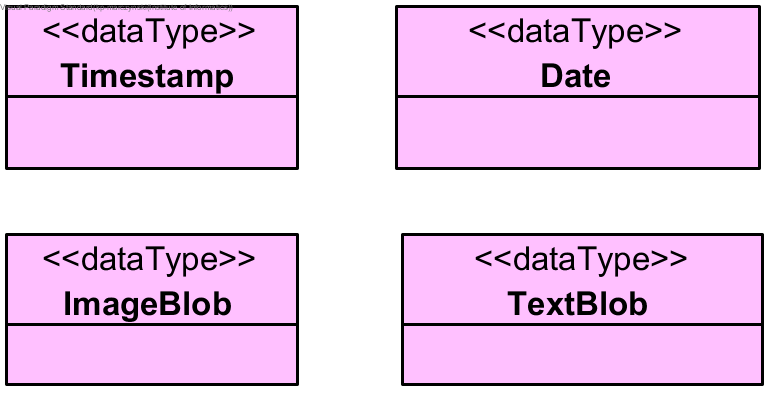
\includegraphics[scale=0.7]{../uml/class_diagrams/dataTypes.png}
        \caption{Typy danych - diagram klas (opr.wł).}\label{rysunek:class-diagram-data-types}
    \end{figure}
\end{minipage}

\begin{minipage}{\textwidth}
    \begin{figure}[H]
        \centering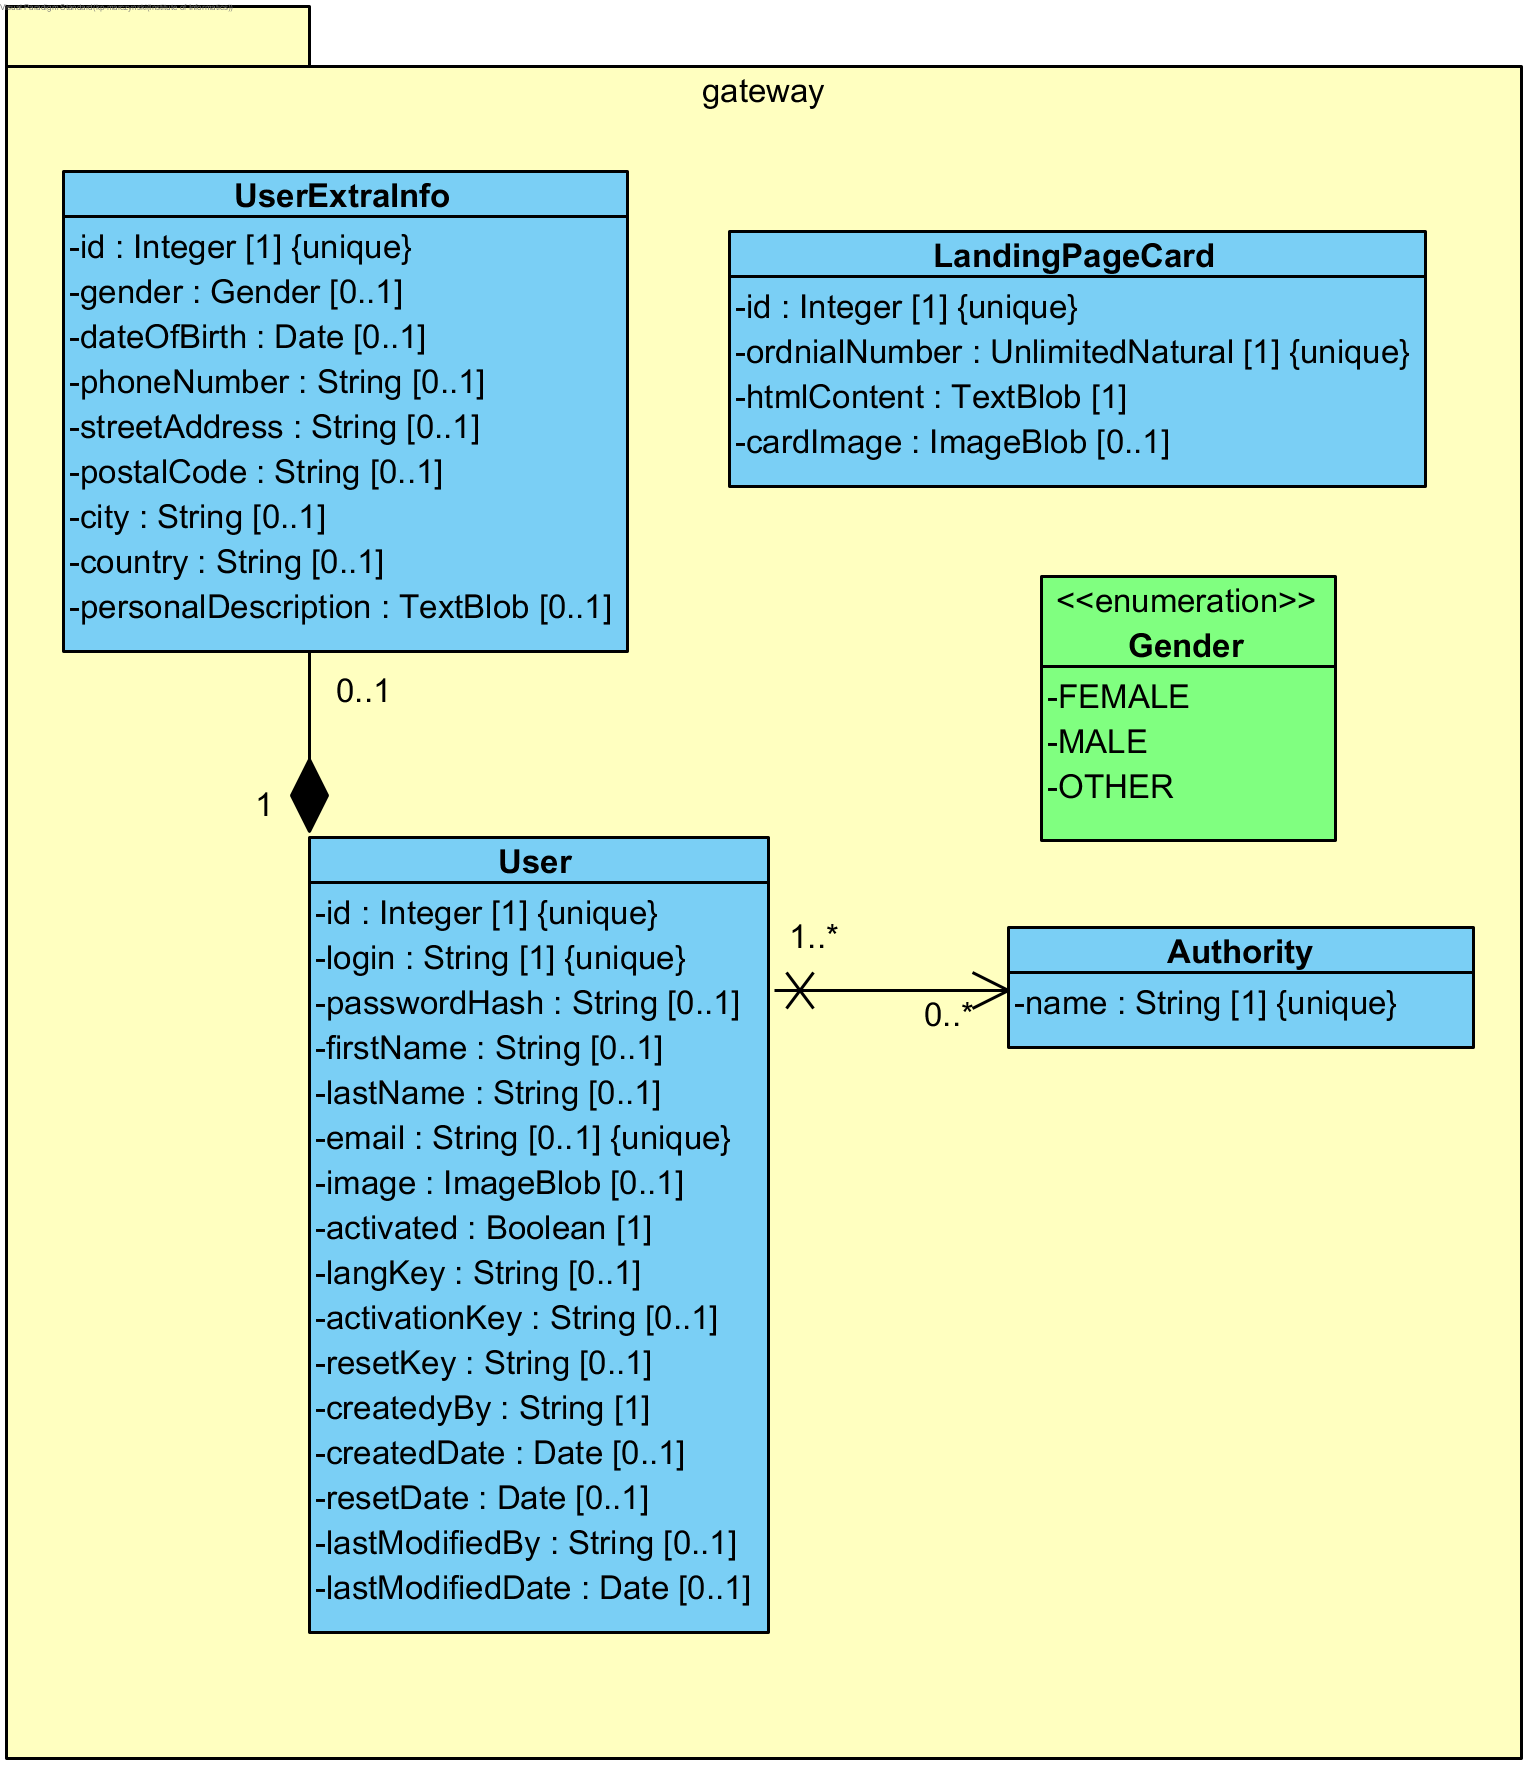
\includegraphics[scale=0.7]{../uml/class_diagrams/gateway.png}
        \caption{Gateway - diagram klas (opr.wł).}\label{rysunek:class-diagram-gateway}
    \end{figure}
\end{minipage}

\begin{minipage}{\textwidth}
    \begin{figure}[H]
        \centering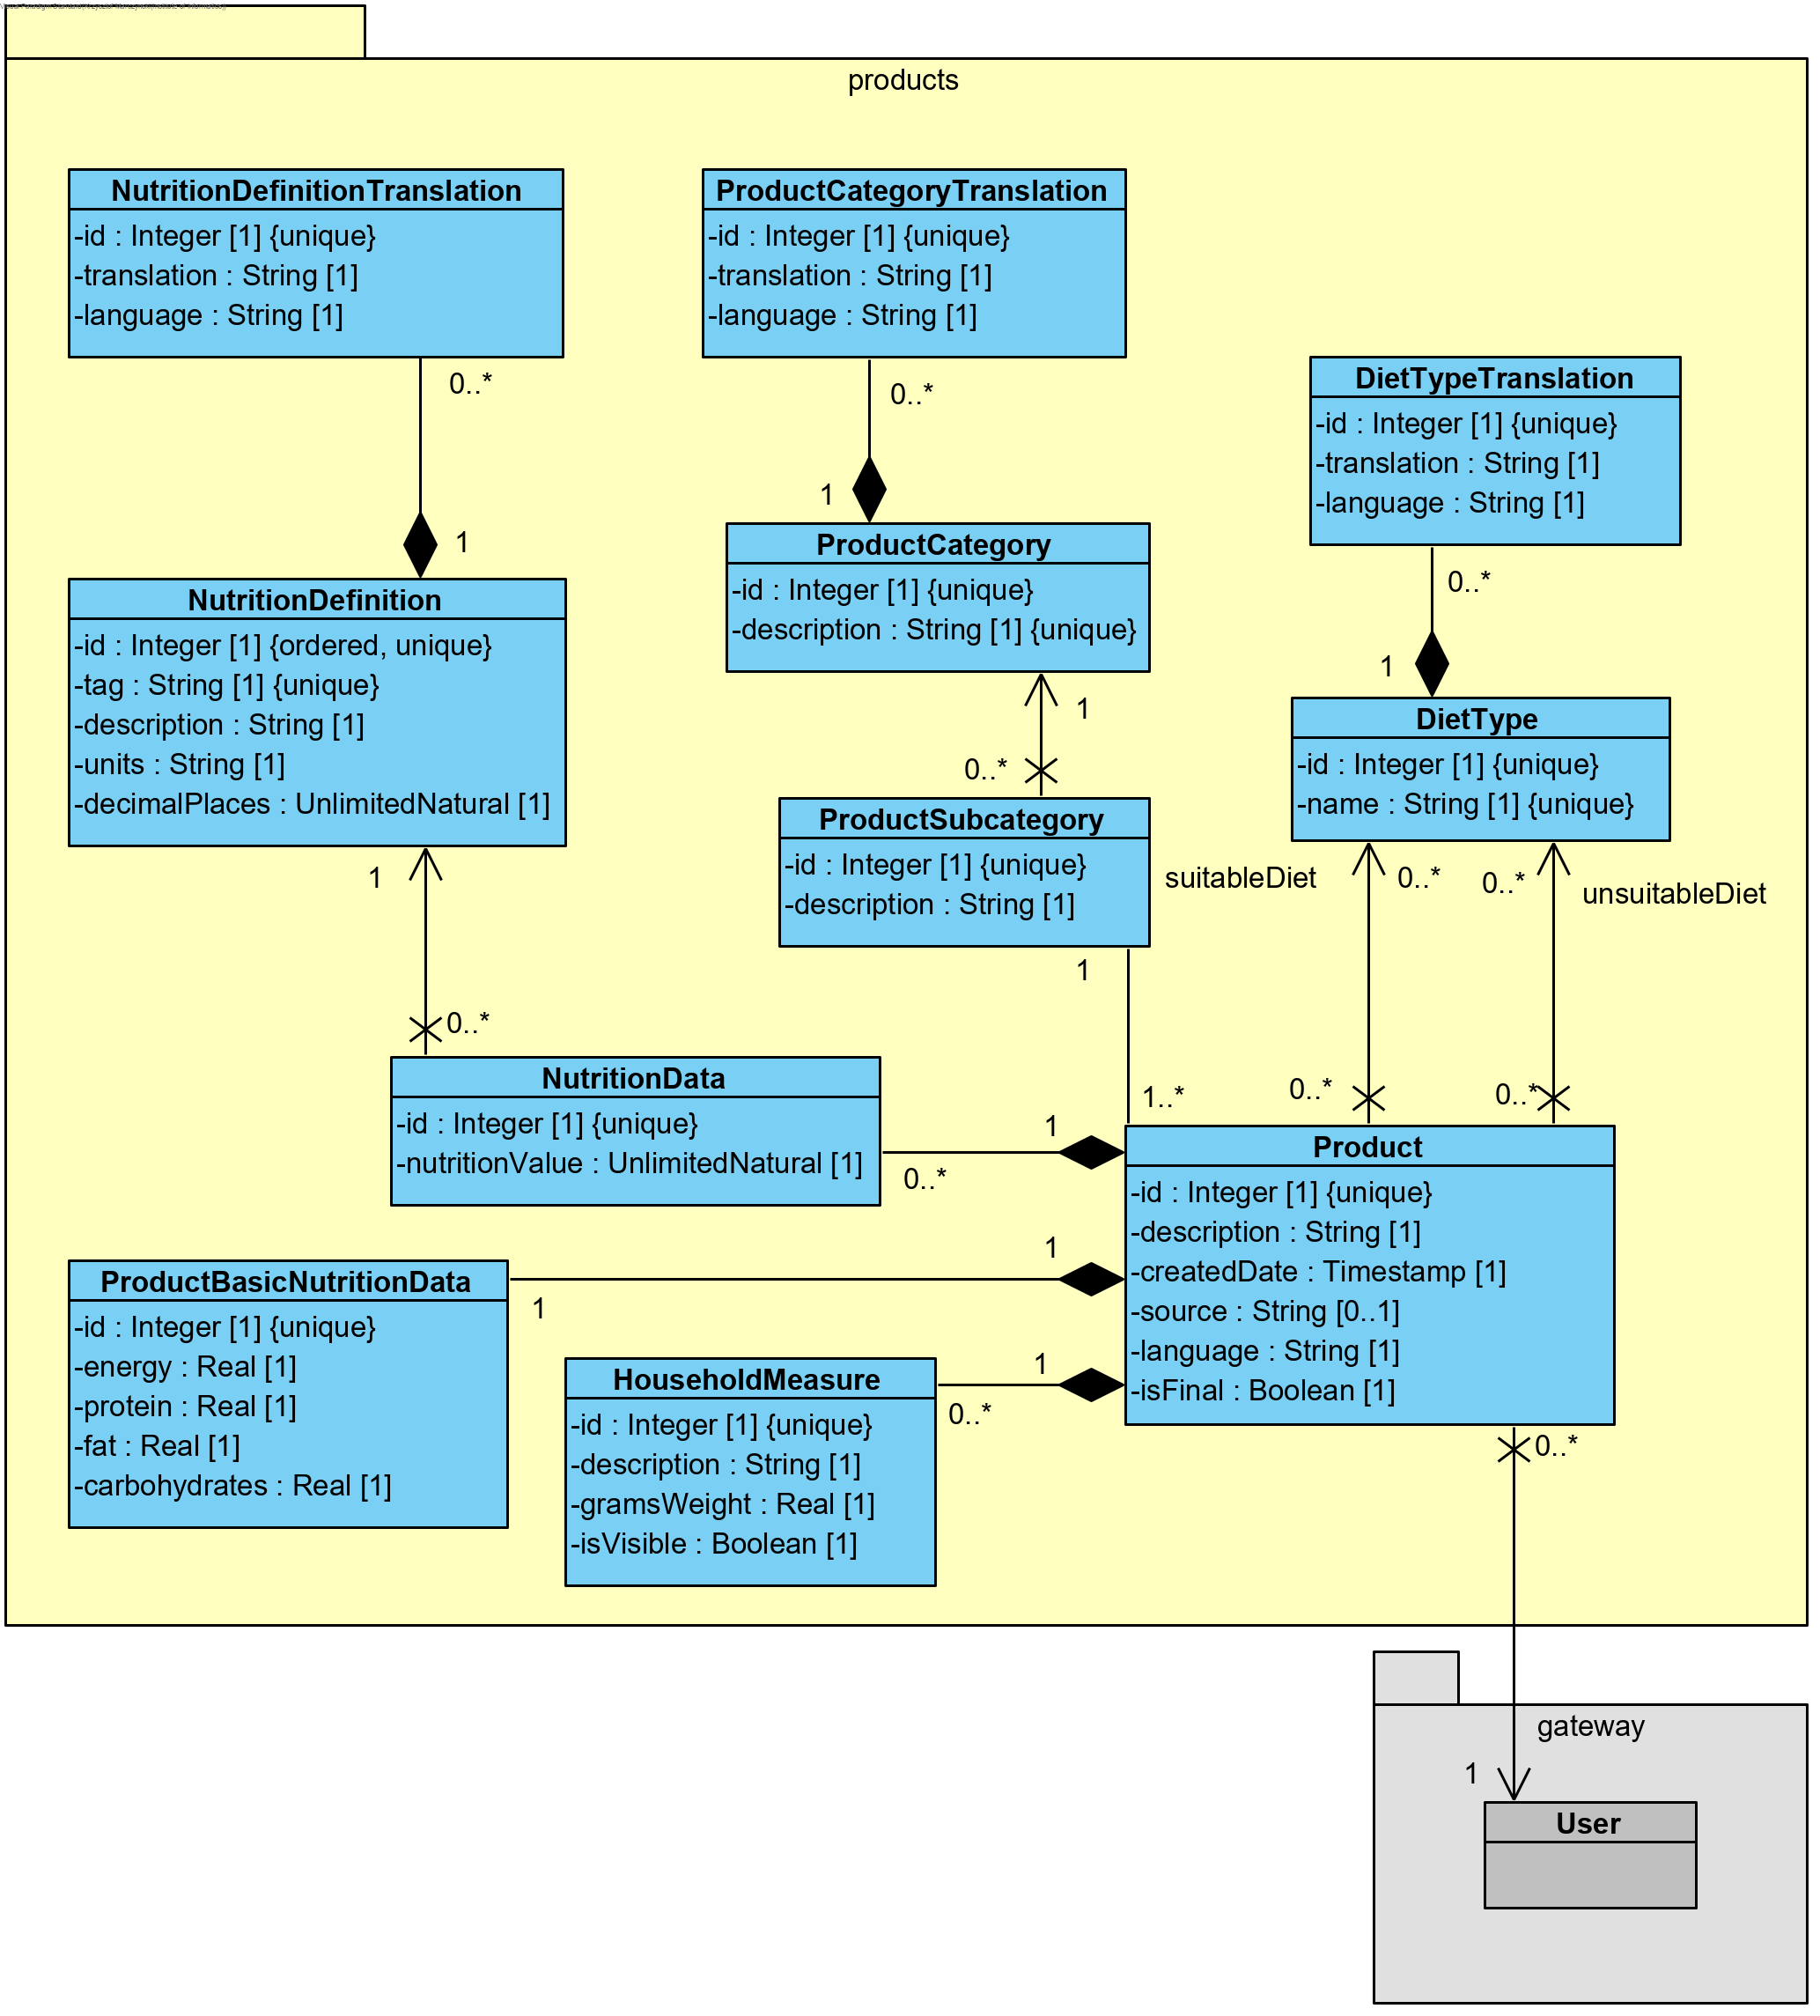
\includegraphics[scale=0.7]{../uml/class_diagrams/products.png}
        \caption{Produkty - diagram klas (opr.wł).}\label{rysunek:class-diagram-products}
    \end{figure}
\end{minipage}

\begin{minipage}{\textwidth}
    \begin{figure}[H]
        \centering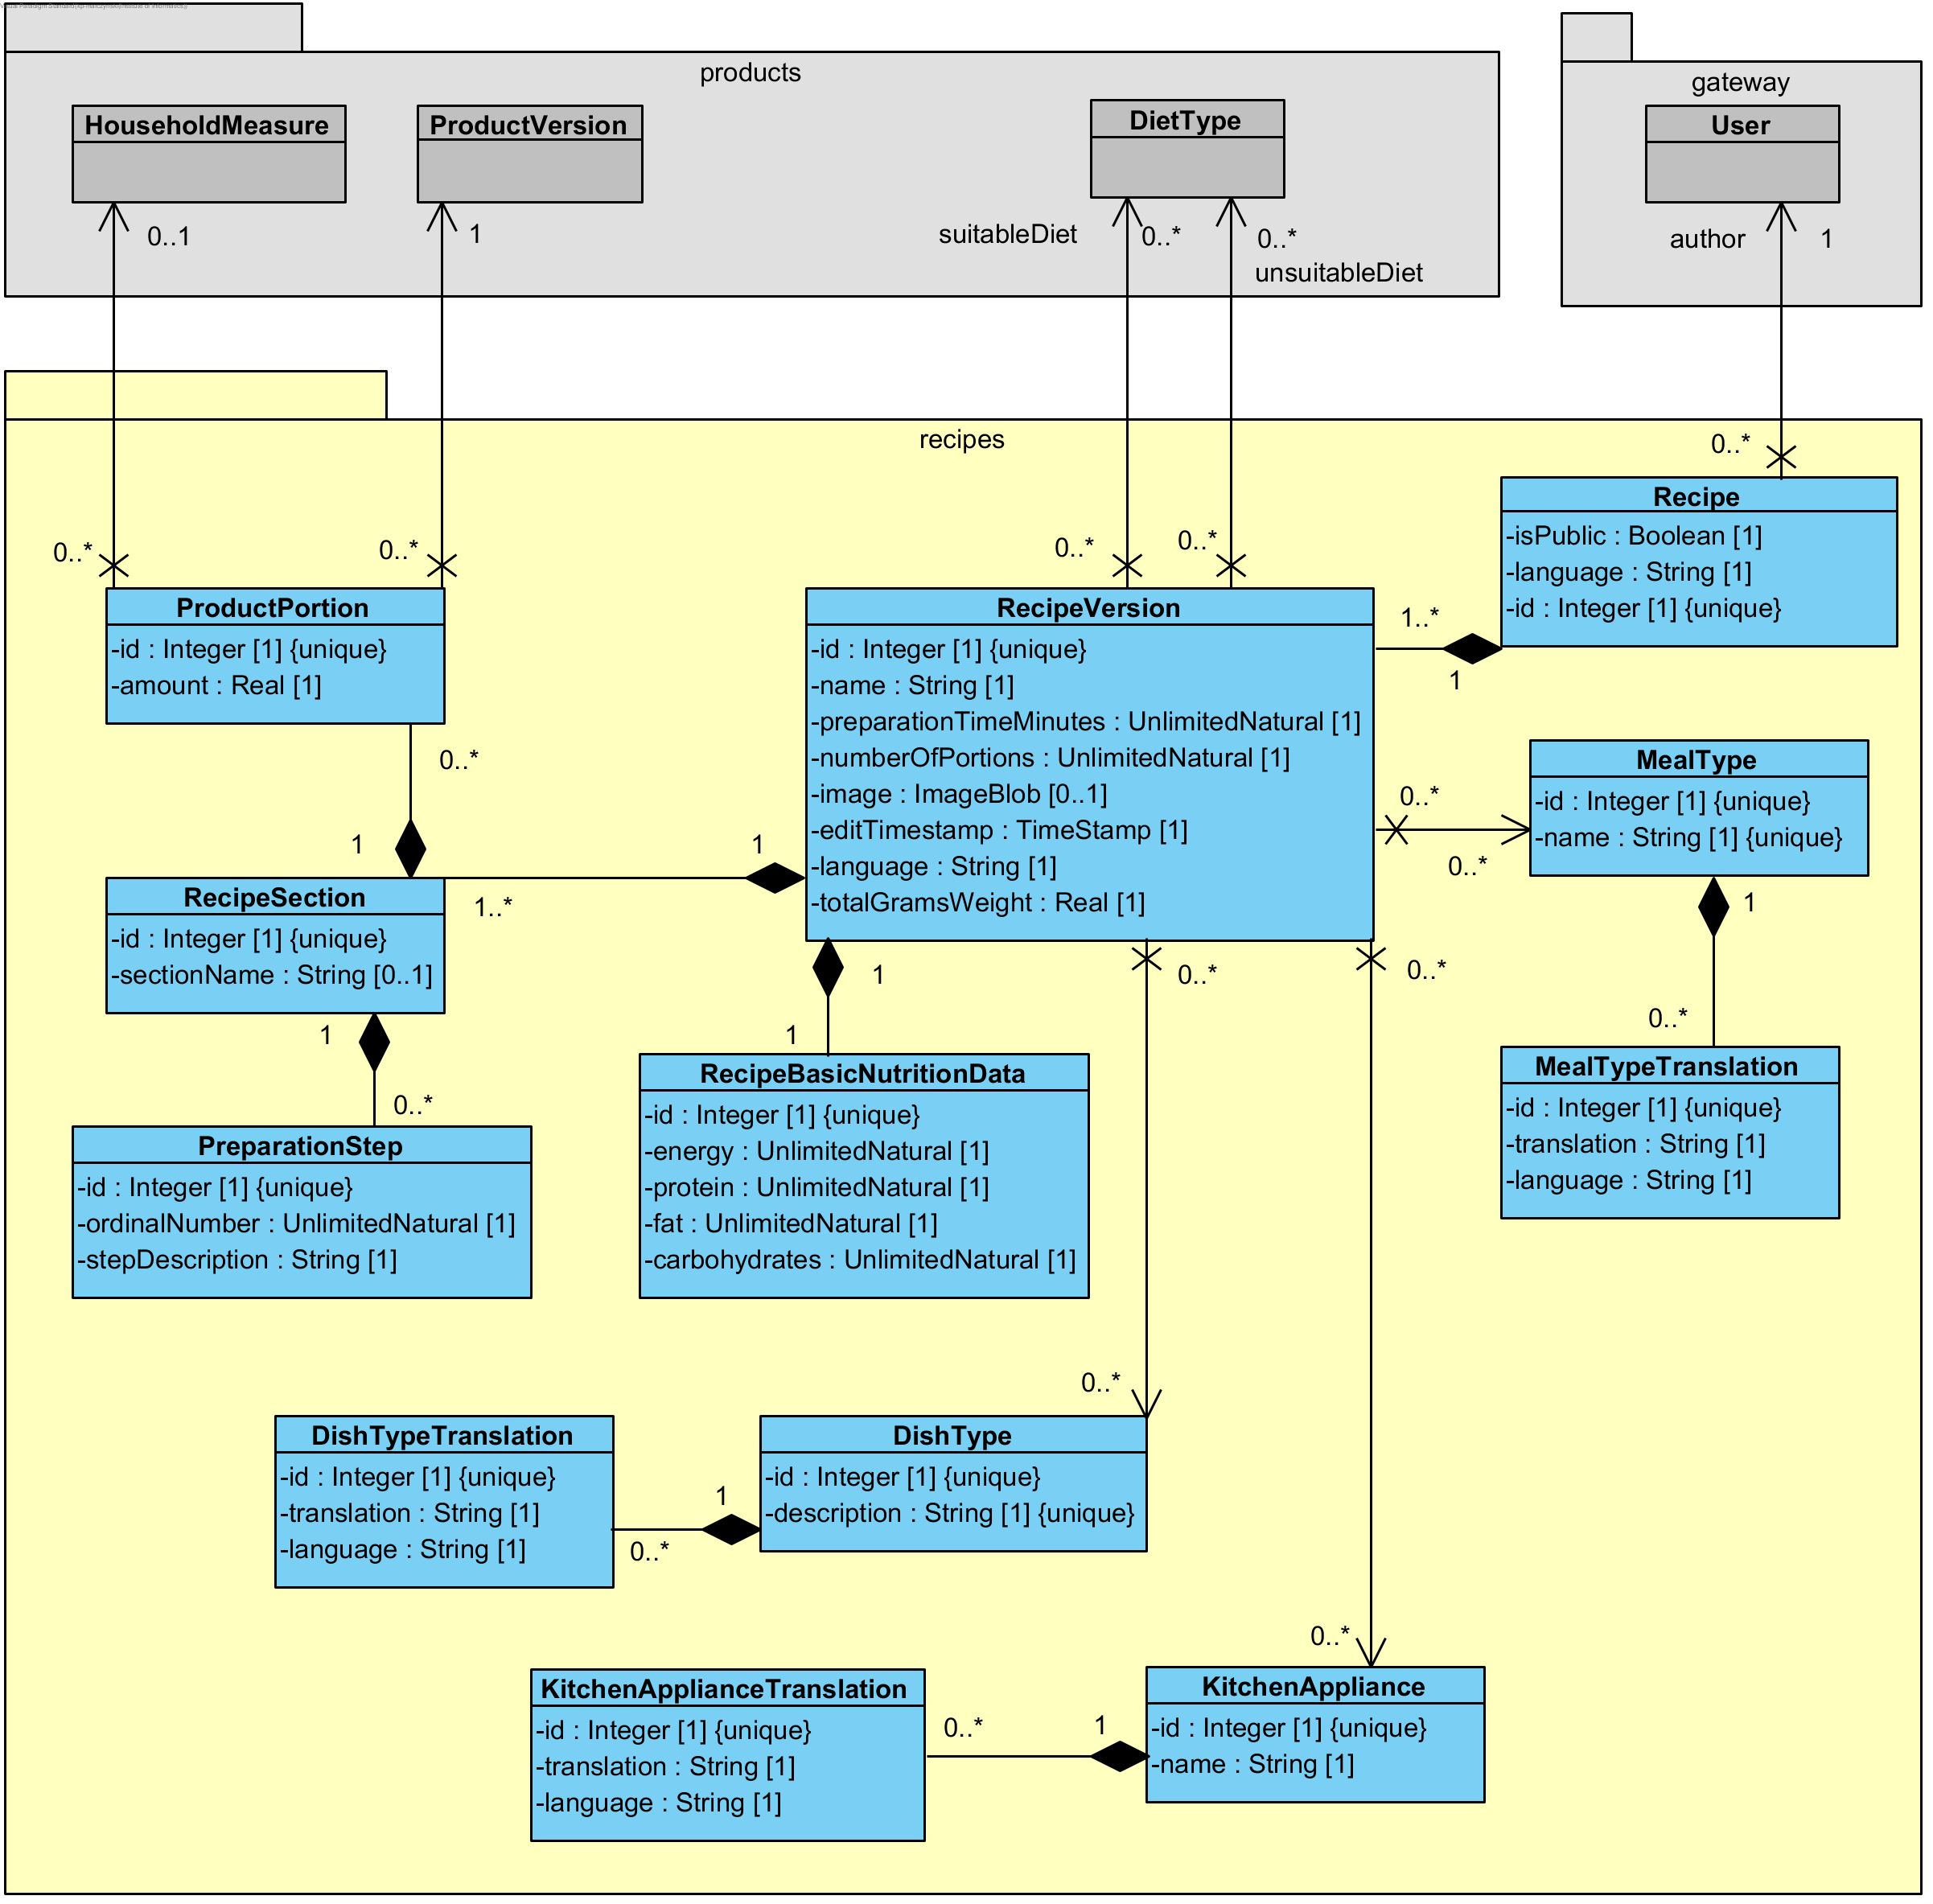
\includegraphics[scale=0.7]{../uml/class_diagrams/recipes.png}
        \caption{Przepisy - diagram klas (opr.wł).}\label{rysunek:class-diagram-recipes}
    \end{figure}
\end{minipage}

\begin{minipage}{\textwidth}
    \begin{figure}[H]
        \centering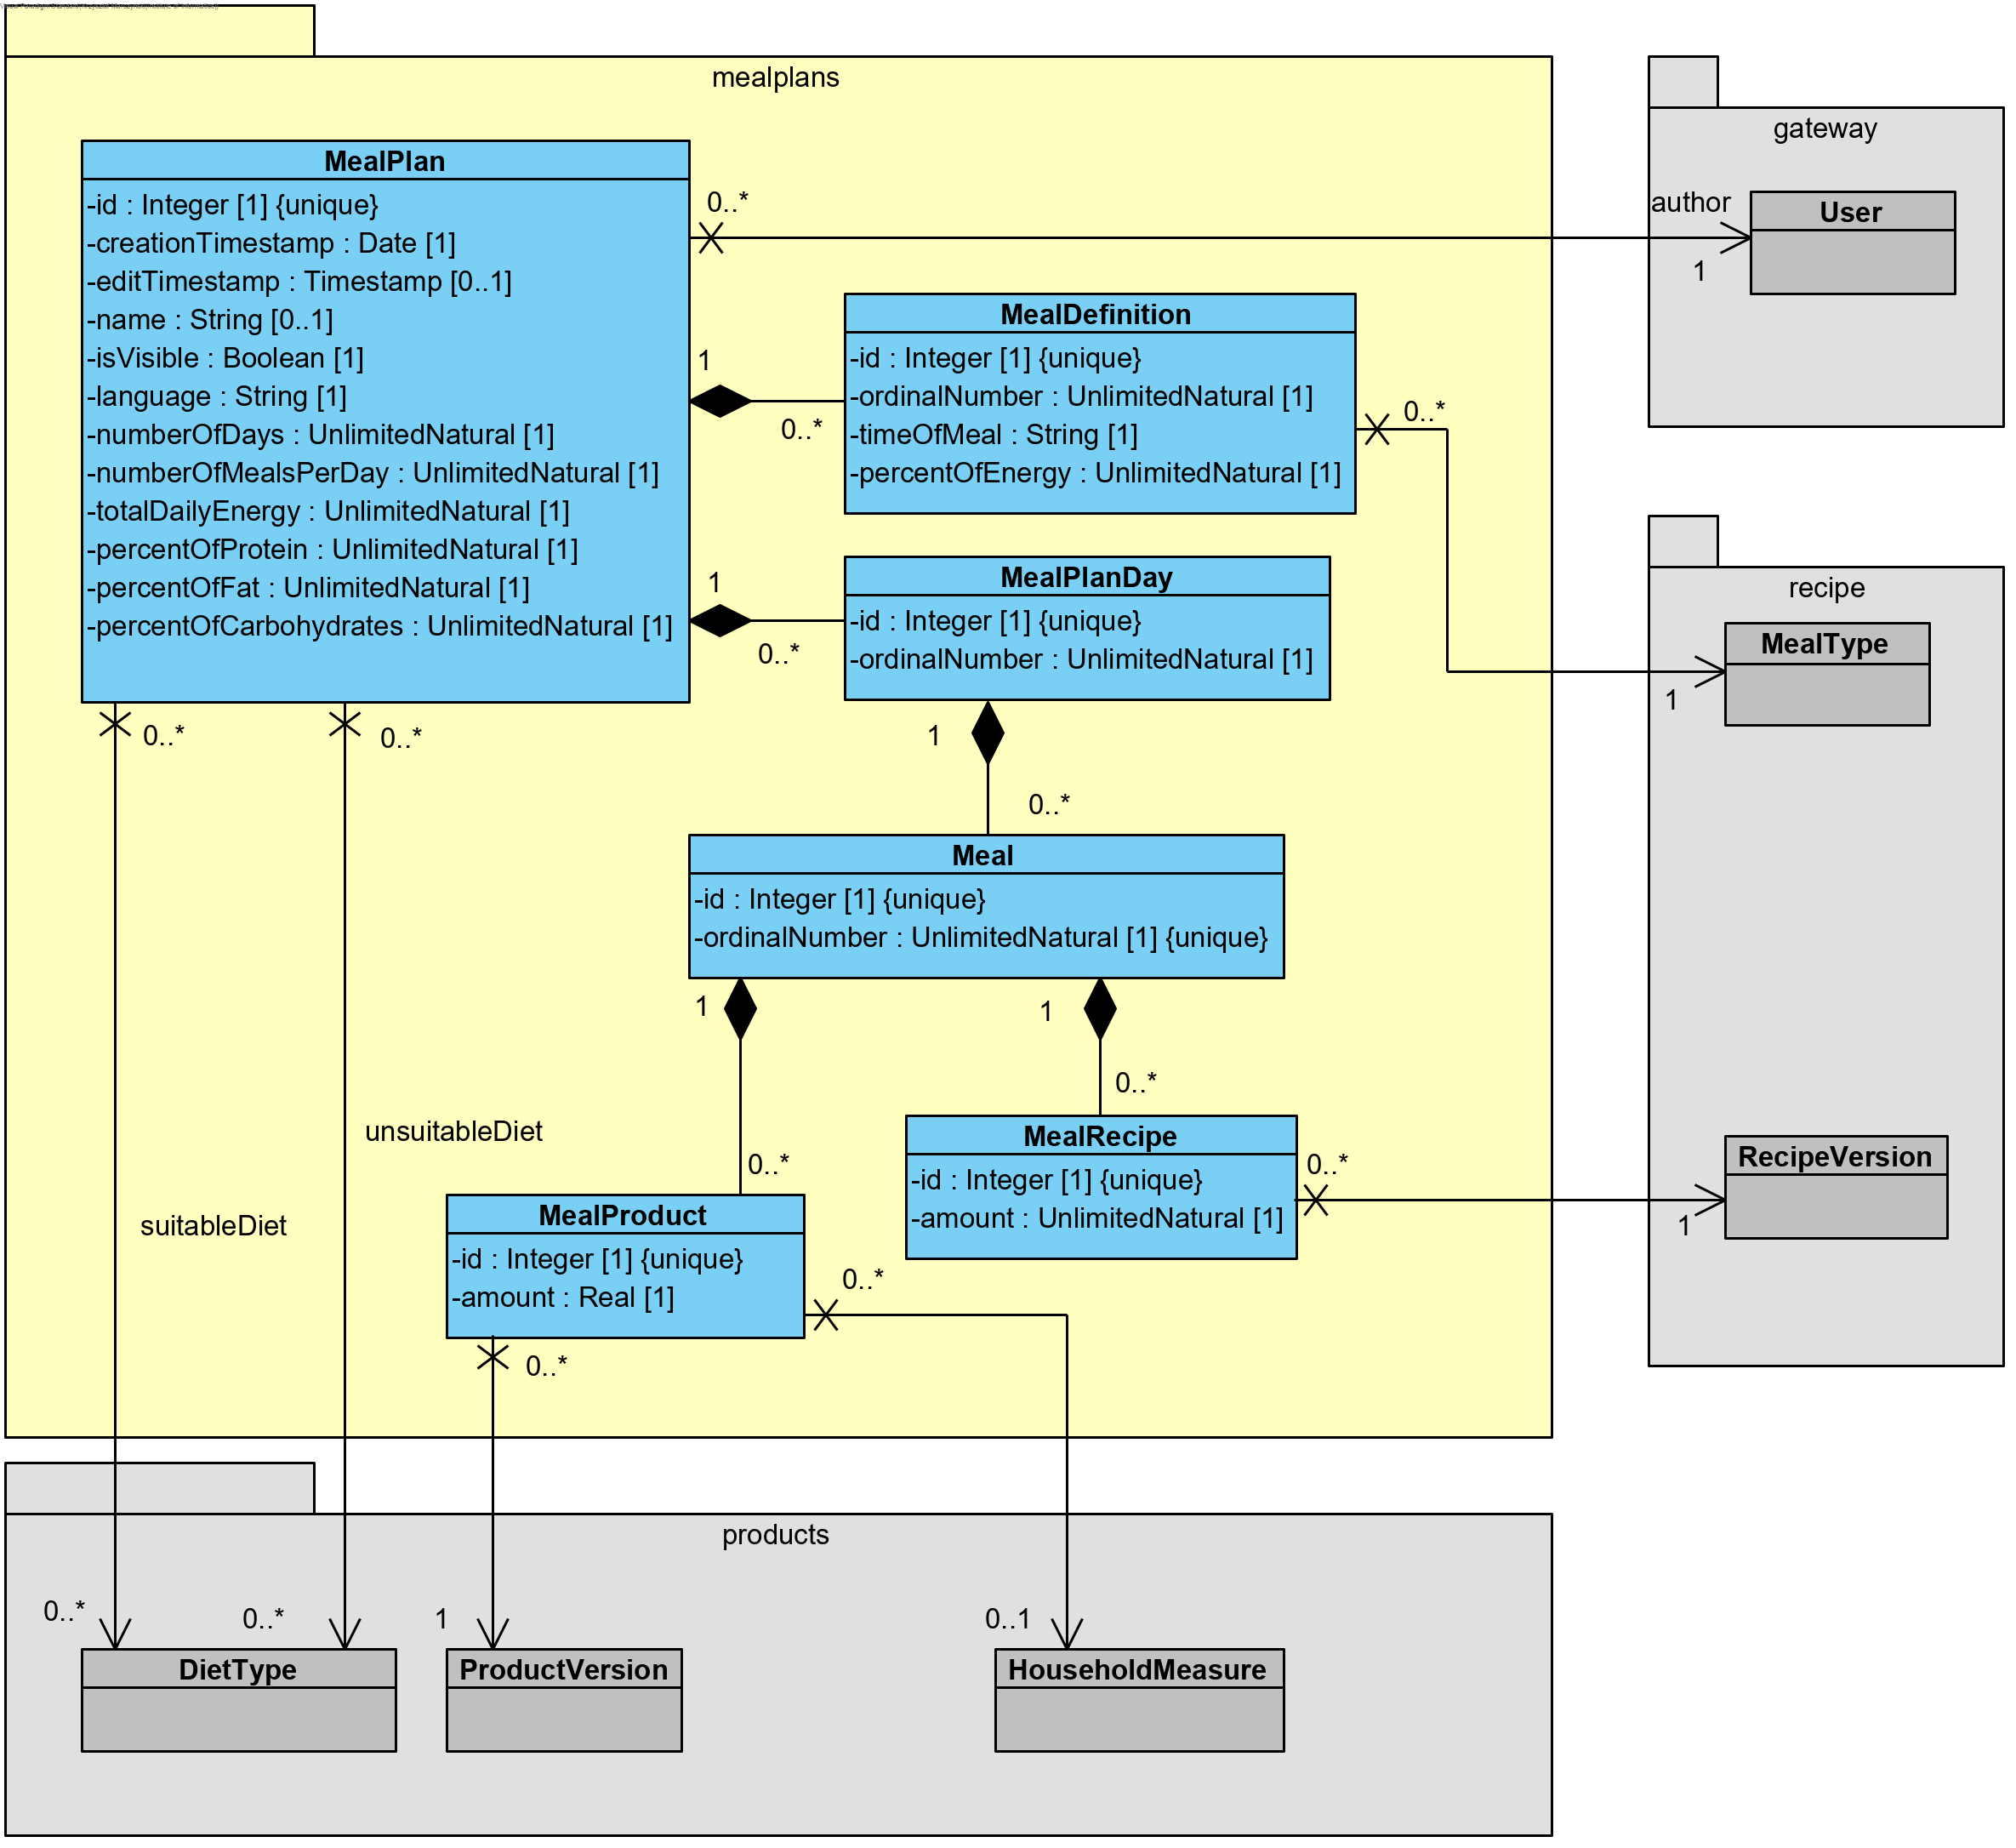
\includegraphics[scale=0.7]{../uml/class_diagrams/mealplans.png}
        \caption{Jadłospisy - diagram klas (opr.wł).}\label{rysunek:class-diagram-mealplans}
    \end{figure}
\end{minipage}

\begin{minipage}{\textwidth}
    \begin{figure}[H]
        \centering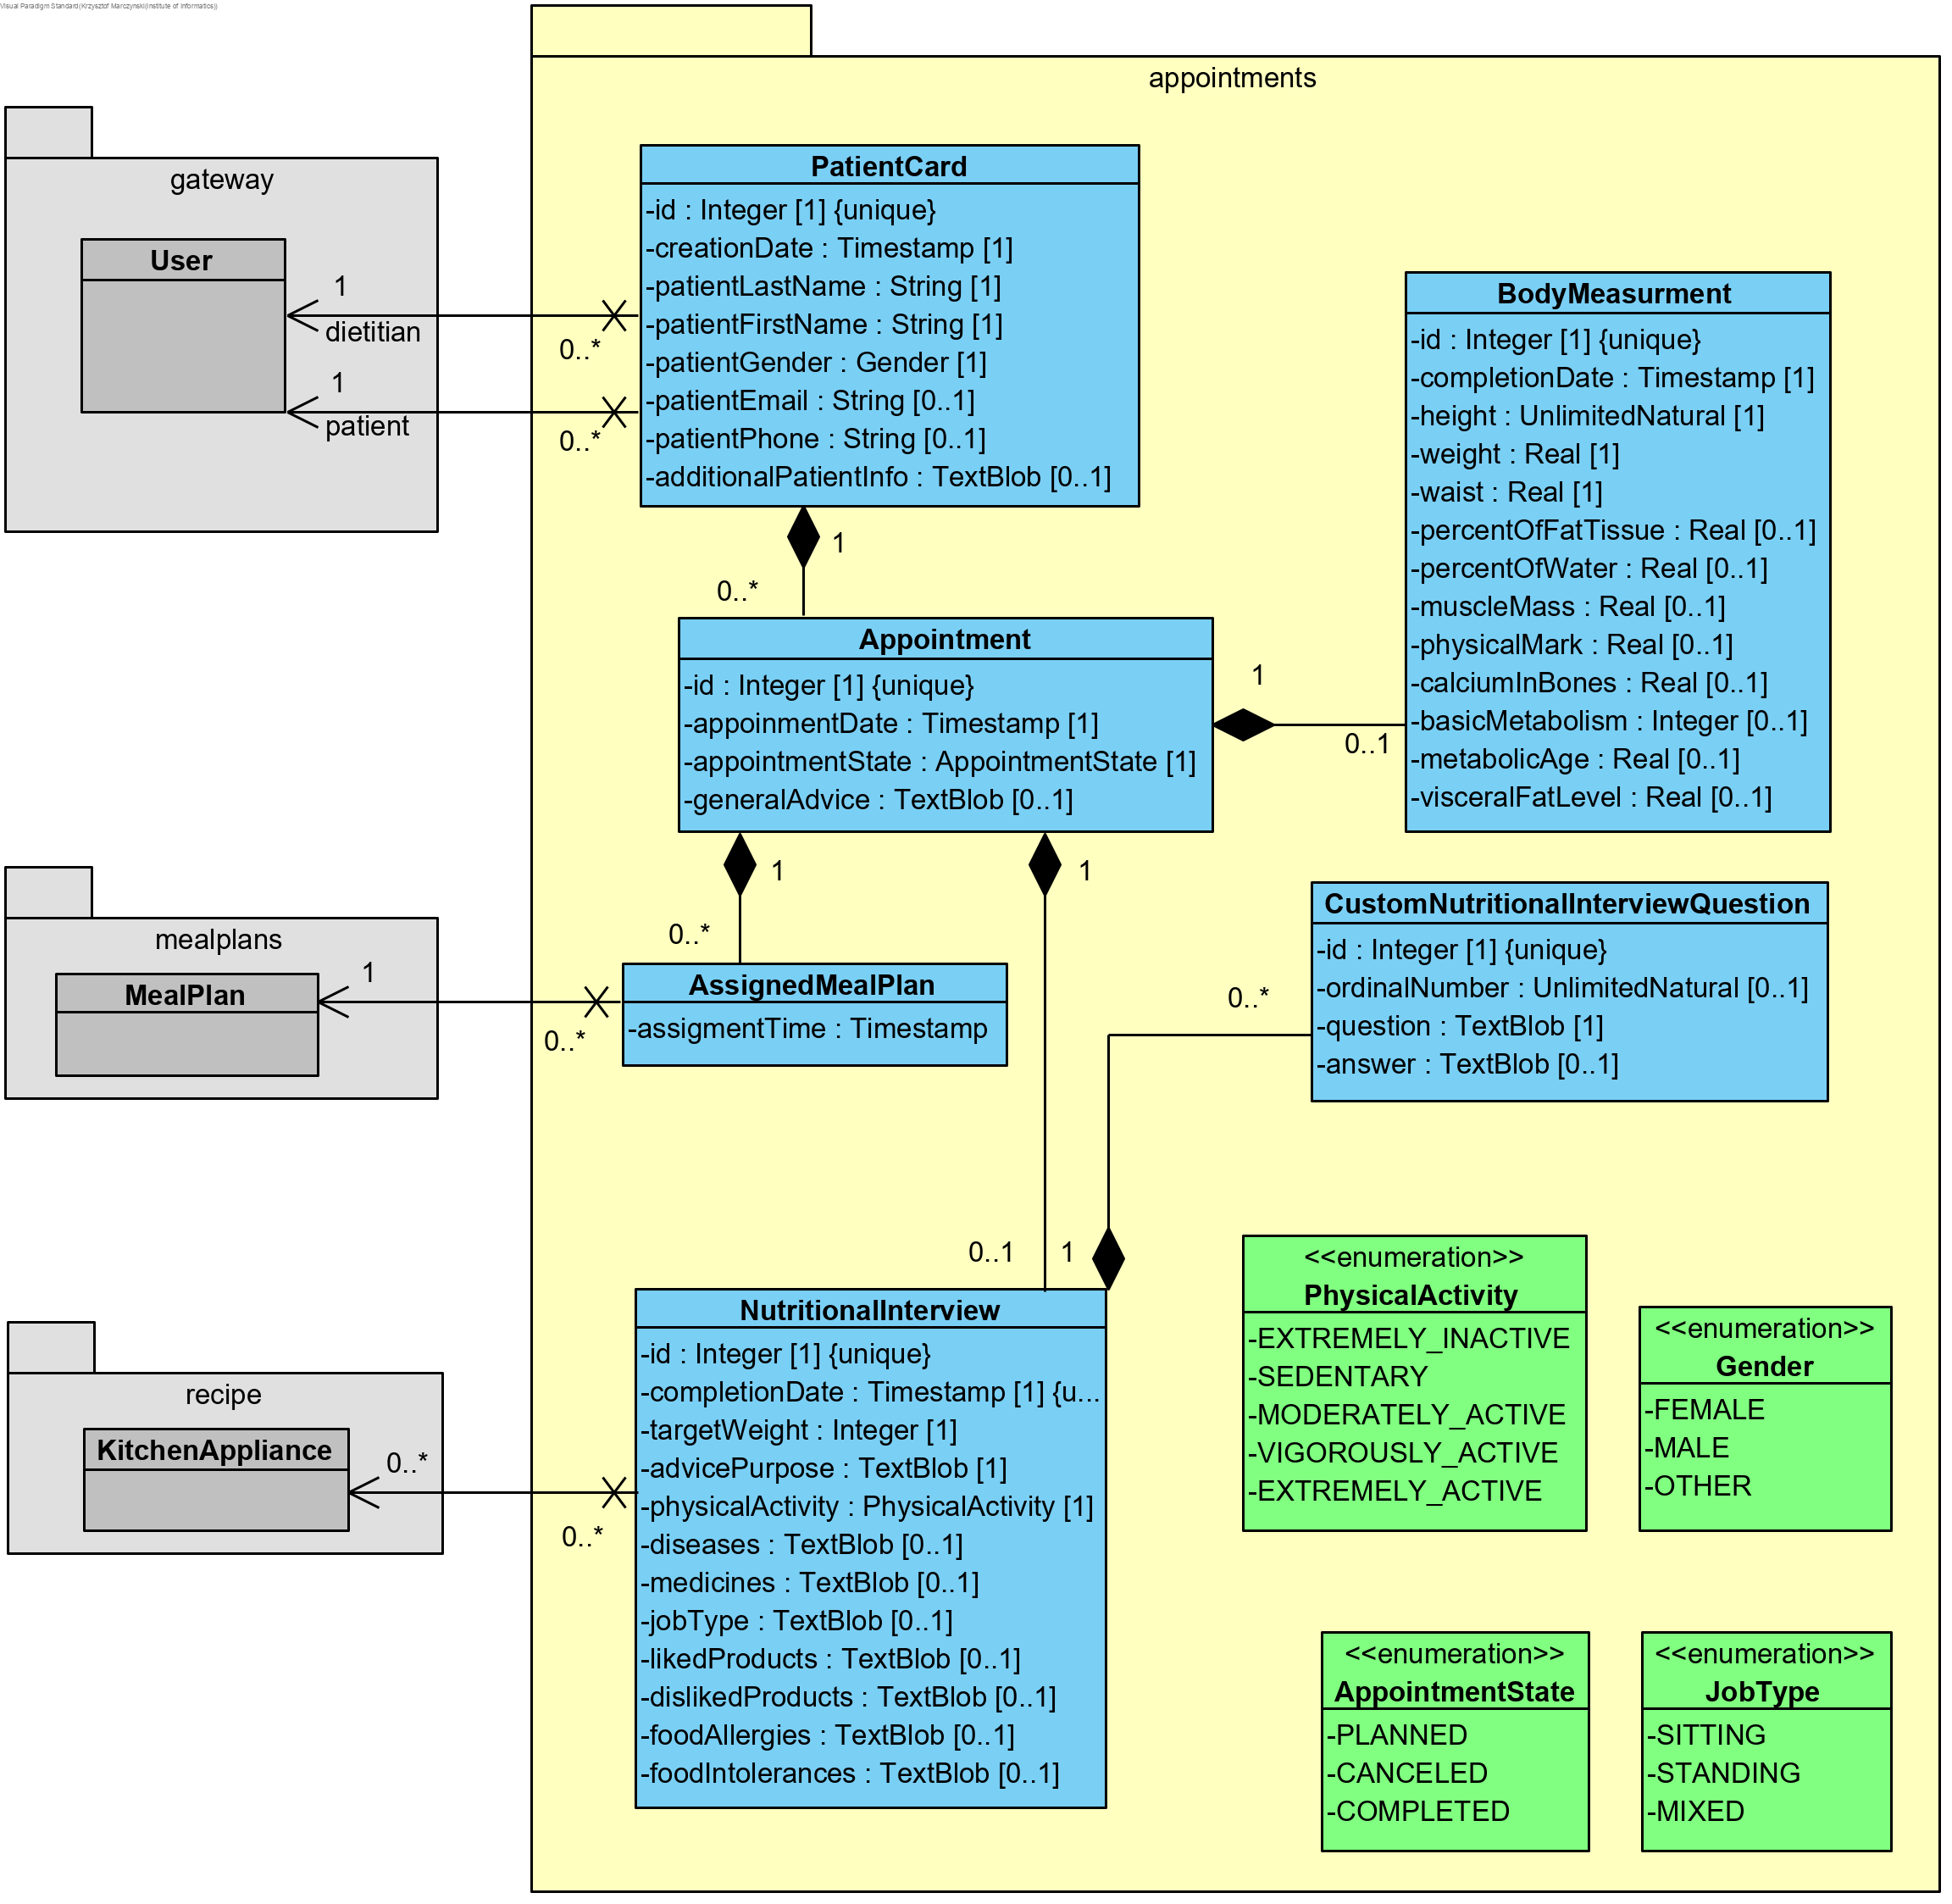
\includegraphics[scale=0.7]{../uml/class_diagrams/appointments.png}
        \caption{Wizyty - diagram klas (opr.wł).}\label{rysunek:class-diagram-appointments}
    \end{figure}
\end{minipage}



\thispagestyle{normal}

\section{Opis podstawowej architektury systemu}
\todo{Opisać, że to aplikacja webowa w architekturze mikroserwisów
Wyszczególnienie modułów;
Diagram rozmieszczenia, wzorce projektowe}

%https://martinfowler.com/eaaDev/TemporalObject.html
\thispagestyle{normal}
